% Options for packages loaded elsewhere
\PassOptionsToPackage{unicode}{hyperref}
\PassOptionsToPackage{hyphens}{url}
%
\documentclass[
]{book}
\usepackage{amsmath,amssymb}
\usepackage{lmodern}
\usepackage{iftex}
\ifPDFTeX
  \usepackage[T1]{fontenc}
  \usepackage[utf8]{inputenc}
  \usepackage{textcomp} % provide euro and other symbols
\else % if luatex or xetex
  \usepackage{unicode-math}
  \defaultfontfeatures{Scale=MatchLowercase}
  \defaultfontfeatures[\rmfamily]{Ligatures=TeX,Scale=1}
\fi
% Use upquote if available, for straight quotes in verbatim environments
\IfFileExists{upquote.sty}{\usepackage{upquote}}{}
\IfFileExists{microtype.sty}{% use microtype if available
  \usepackage[]{microtype}
  \UseMicrotypeSet[protrusion]{basicmath} % disable protrusion for tt fonts
}{}
\makeatletter
\@ifundefined{KOMAClassName}{% if non-KOMA class
  \IfFileExists{parskip.sty}{%
    \usepackage{parskip}
  }{% else
    \setlength{\parindent}{0pt}
    \setlength{\parskip}{6pt plus 2pt minus 1pt}}
}{% if KOMA class
  \KOMAoptions{parskip=half}}
\makeatother
\usepackage{xcolor}
\usepackage{color}
\usepackage{fancyvrb}
\newcommand{\VerbBar}{|}
\newcommand{\VERB}{\Verb[commandchars=\\\{\}]}
\DefineVerbatimEnvironment{Highlighting}{Verbatim}{commandchars=\\\{\}}
% Add ',fontsize=\small' for more characters per line
\usepackage{framed}
\definecolor{shadecolor}{RGB}{248,248,248}
\newenvironment{Shaded}{\begin{snugshade}}{\end{snugshade}}
\newcommand{\AlertTok}[1]{\textcolor[rgb]{0.94,0.16,0.16}{#1}}
\newcommand{\AnnotationTok}[1]{\textcolor[rgb]{0.56,0.35,0.01}{\textbf{\textit{#1}}}}
\newcommand{\AttributeTok}[1]{\textcolor[rgb]{0.77,0.63,0.00}{#1}}
\newcommand{\BaseNTok}[1]{\textcolor[rgb]{0.00,0.00,0.81}{#1}}
\newcommand{\BuiltInTok}[1]{#1}
\newcommand{\CharTok}[1]{\textcolor[rgb]{0.31,0.60,0.02}{#1}}
\newcommand{\CommentTok}[1]{\textcolor[rgb]{0.56,0.35,0.01}{\textit{#1}}}
\newcommand{\CommentVarTok}[1]{\textcolor[rgb]{0.56,0.35,0.01}{\textbf{\textit{#1}}}}
\newcommand{\ConstantTok}[1]{\textcolor[rgb]{0.00,0.00,0.00}{#1}}
\newcommand{\ControlFlowTok}[1]{\textcolor[rgb]{0.13,0.29,0.53}{\textbf{#1}}}
\newcommand{\DataTypeTok}[1]{\textcolor[rgb]{0.13,0.29,0.53}{#1}}
\newcommand{\DecValTok}[1]{\textcolor[rgb]{0.00,0.00,0.81}{#1}}
\newcommand{\DocumentationTok}[1]{\textcolor[rgb]{0.56,0.35,0.01}{\textbf{\textit{#1}}}}
\newcommand{\ErrorTok}[1]{\textcolor[rgb]{0.64,0.00,0.00}{\textbf{#1}}}
\newcommand{\ExtensionTok}[1]{#1}
\newcommand{\FloatTok}[1]{\textcolor[rgb]{0.00,0.00,0.81}{#1}}
\newcommand{\FunctionTok}[1]{\textcolor[rgb]{0.00,0.00,0.00}{#1}}
\newcommand{\ImportTok}[1]{#1}
\newcommand{\InformationTok}[1]{\textcolor[rgb]{0.56,0.35,0.01}{\textbf{\textit{#1}}}}
\newcommand{\KeywordTok}[1]{\textcolor[rgb]{0.13,0.29,0.53}{\textbf{#1}}}
\newcommand{\NormalTok}[1]{#1}
\newcommand{\OperatorTok}[1]{\textcolor[rgb]{0.81,0.36,0.00}{\textbf{#1}}}
\newcommand{\OtherTok}[1]{\textcolor[rgb]{0.56,0.35,0.01}{#1}}
\newcommand{\PreprocessorTok}[1]{\textcolor[rgb]{0.56,0.35,0.01}{\textit{#1}}}
\newcommand{\RegionMarkerTok}[1]{#1}
\newcommand{\SpecialCharTok}[1]{\textcolor[rgb]{0.00,0.00,0.00}{#1}}
\newcommand{\SpecialStringTok}[1]{\textcolor[rgb]{0.31,0.60,0.02}{#1}}
\newcommand{\StringTok}[1]{\textcolor[rgb]{0.31,0.60,0.02}{#1}}
\newcommand{\VariableTok}[1]{\textcolor[rgb]{0.00,0.00,0.00}{#1}}
\newcommand{\VerbatimStringTok}[1]{\textcolor[rgb]{0.31,0.60,0.02}{#1}}
\newcommand{\WarningTok}[1]{\textcolor[rgb]{0.56,0.35,0.01}{\textbf{\textit{#1}}}}
\usepackage{longtable,booktabs,array}
\usepackage{calc} % for calculating minipage widths
% Correct order of tables after \paragraph or \subparagraph
\usepackage{etoolbox}
\makeatletter
\patchcmd\longtable{\par}{\if@noskipsec\mbox{}\fi\par}{}{}
\makeatother
% Allow footnotes in longtable head/foot
\IfFileExists{footnotehyper.sty}{\usepackage{footnotehyper}}{\usepackage{footnote}}
\makesavenoteenv{longtable}
\usepackage{graphicx}
\makeatletter
\def\maxwidth{\ifdim\Gin@nat@width>\linewidth\linewidth\else\Gin@nat@width\fi}
\def\maxheight{\ifdim\Gin@nat@height>\textheight\textheight\else\Gin@nat@height\fi}
\makeatother
% Scale images if necessary, so that they will not overflow the page
% margins by default, and it is still possible to overwrite the defaults
% using explicit options in \includegraphics[width, height, ...]{}
\setkeys{Gin}{width=\maxwidth,height=\maxheight,keepaspectratio}
% Set default figure placement to htbp
\makeatletter
\def\fps@figure{htbp}
\makeatother
\setlength{\emergencystretch}{3em} % prevent overfull lines
\providecommand{\tightlist}{%
  \setlength{\itemsep}{0pt}\setlength{\parskip}{0pt}}
\setcounter{secnumdepth}{5}
\usepackage{booktabs}
\ifLuaTeX
  \usepackage{selnolig}  % disable illegal ligatures
\fi
\usepackage[]{natbib}
\bibliographystyle{plainnat}
\IfFileExists{bookmark.sty}{\usepackage{bookmark}}{\usepackage{hyperref}}
\IfFileExists{xurl.sty}{\usepackage{xurl}}{} % add URL line breaks if available
\urlstyle{same} % disable monospaced font for URLs
\hypersetup{
  pdftitle={Learning R packages},
  pdfauthor={Cristian Villegas},
  hidelinks,
  pdfcreator={LaTeX via pandoc}}

\title{Learning R packages}
\author{Cristian Villegas}
\date{2023-05-09}

\begin{document}
\maketitle

{
\setcounter{tocdepth}{1}
\tableofcontents
}
\hypertarget{intro}{%
\chapter{Intro}\label{intro}}

\hypertarget{carrega-pacotes-a-serem-usados}{%
\section{Carrega pacotes a serem usados}\label{carrega-pacotes-a-serem-usados}}

\begin{Shaded}
\begin{Highlighting}[]
\CommentTok{\#install.packages("tidyverse") }
\CommentTok{\#install.packages("dplyr")     }
\CommentTok{\#install.packages("tidyr")     }
\CommentTok{\#install.packages("ggplot2")   }

\FunctionTok{library}\NormalTok{(tidyverse)}
\CommentTok{\# Manipulação de dados}
\CommentTok{\#library(dplyr)}

\CommentTok{\# Visualização de gráficos}
\FunctionTok{library}\NormalTok{(ggplot2)}
\FunctionTok{library}\NormalTok{(gridExtra)}
\FunctionTok{library}\NormalTok{(patchwork)}
\FunctionTok{library}\NormalTok{(plotly)}
\FunctionTok{library}\NormalTok{(esquisse)}

\CommentTok{\# Para dados gráfico de perfis}
\FunctionTok{library}\NormalTok{(nlme)}
\end{Highlighting}
\end{Shaded}

Ver como citar referências \citet{tidyverse2019}, \citet{R-tidyverse}, \citet{R-tidyr}, \citet{R-ggplot2}, \citet{R-purrr}, \citet{R-dplyr}, \citet{R-knitr}, \citet{R-bookdown}

\hypertarget{alguns-atalhos-no-rstudio}{%
\section{Alguns atalhos no Rstudio}\label{alguns-atalhos-no-rstudio}}

Para considerar

\begin{quote}
Operador Pipe (\%\textgreater\%): Ctrl + Shift + M (Windows) ou Cmd + Shift + M (Mac).
\end{quote}

\begin{quote}
Criar novos chunks: Ctrl + Alt + I (Windows) ou Cmd + Option + I (Mac).
\end{quote}

\hypertarget{descriuxe7uxe3o-dos-dados-mpg}{%
\section{\texorpdfstring{Descrição dos dados \texttt{mpg}}{Descrição dos dados mpg}}\label{descriuxe7uxe3o-dos-dados-mpg}}

Dados de economia de combustível de 1999 a 2008 para \emph{38 modelos populares de carros}. Este conjunto de dados contém um subconjunto dos dados de economia de combustível que a EPA disponibiliza em \emph{\url{https://fueleconomy.gov/}}. Ele contém apenas modelos que tiveram um novo lançamento a cada ano entre 1999 e 2008 - isso foi usado como um substituto para a popularidade do carro. Um \emph{data frame} com 234 linhas e 11 variáveis:

\begin{itemize}
\item
  \emph{manufacturer} nome do fabricante
\item
  \emph{model} nome do modelo
\item
  \emph{displ} cilindrada do motor, em litros
\item
  \emph{year} ano de fabricação
\item
  \emph{cyl} número de cilindros
\item
  \emph{trans} tipo de transmissão
\item
  \emph{drv} o tipo de trem de força, onde \textbf{f = tração dianteira}, \textbf{r = tração traseira} e \textbf{4 = 4wd}
\item
  \emph{cty} milhas urbanas por galão
\item
  \emph{hwy} milhas rodoviárias por galão
\item
  \emph{fl} tipo de combustível
\item
  \emph{class} ``tipo'' de carro
\end{itemize}

\begin{Shaded}
\begin{Highlighting}[]
\CommentTok{\#help("mpg")}
\NormalTok{dados }\OtherTok{\textless{}{-}}\NormalTok{ mpg}
\FunctionTok{glimpse}\NormalTok{(dados)}
\end{Highlighting}
\end{Shaded}

\begin{verbatim}
## Rows: 234
## Columns: 11
## $ manufacturer <chr> "audi", "audi", "audi", "audi", "audi", "audi", "audi", "~
## $ model        <chr> "a4", "a4", "a4", "a4", "a4", "a4", "a4", "a4 quattro", "~
## $ displ        <dbl> 1.8, 1.8, 2.0, 2.0, 2.8, 2.8, 3.1, 1.8, 1.8, 2.0, 2.0, 2.~
## $ year         <int> 1999, 1999, 2008, 2008, 1999, 1999, 2008, 1999, 1999, 200~
## $ cyl          <int> 4, 4, 4, 4, 6, 6, 6, 4, 4, 4, 4, 6, 6, 6, 6, 6, 6, 8, 8, ~
## $ trans        <chr> "auto(l5)", "manual(m5)", "manual(m6)", "auto(av)", "auto~
## $ drv          <chr> "f", "f", "f", "f", "f", "f", "f", "4", "4", "4", "4", "4~
## $ cty          <int> 18, 21, 20, 21, 16, 18, 18, 18, 16, 20, 19, 15, 17, 17, 1~
## $ hwy          <int> 29, 29, 31, 30, 26, 26, 27, 26, 25, 28, 27, 25, 25, 25, 2~
## $ fl           <chr> "p", "p", "p", "p", "p", "p", "p", "p", "p", "p", "p", "p~
## $ class        <chr> "compact", "compact", "compact", "compact", "compact", "c~
\end{verbatim}

\begin{Shaded}
\begin{Highlighting}[]
\NormalTok{dados }\OtherTok{\textless{}{-}} \FunctionTok{mutate}\NormalTok{(}\AttributeTok{.data =}\NormalTok{ dados, }
                \FunctionTok{across}\NormalTok{(}\FunctionTok{where}\NormalTok{(is.character), }
\NormalTok{                as.factor))}
\CommentTok{\#View(df) }
\FunctionTok{glimpse}\NormalTok{(dados)}
\end{Highlighting}
\end{Shaded}

\begin{verbatim}
## Rows: 234
## Columns: 11
## $ manufacturer <fct> audi, audi, audi, audi, audi, audi, audi, audi, audi, aud~
## $ model        <fct> a4, a4, a4, a4, a4, a4, a4, a4 quattro, a4 quattro, a4 qu~
## $ displ        <dbl> 1.8, 1.8, 2.0, 2.0, 2.8, 2.8, 3.1, 1.8, 1.8, 2.0, 2.0, 2.~
## $ year         <int> 1999, 1999, 2008, 2008, 1999, 1999, 2008, 1999, 1999, 200~
## $ cyl          <int> 4, 4, 4, 4, 6, 6, 6, 4, 4, 4, 4, 6, 6, 6, 6, 6, 6, 8, 8, ~
## $ trans        <fct> auto(l5), manual(m5), manual(m6), auto(av), auto(l5), man~
## $ drv          <fct> f, f, f, f, f, f, f, 4, 4, 4, 4, 4, 4, 4, 4, 4, 4, 4, r, ~
## $ cty          <int> 18, 21, 20, 21, 16, 18, 18, 18, 16, 20, 19, 15, 17, 17, 1~
## $ hwy          <int> 29, 29, 31, 30, 26, 26, 27, 26, 25, 28, 27, 25, 25, 25, 2~
## $ fl           <fct> p, p, p, p, p, p, p, p, p, p, p, p, p, p, p, p, p, p, r, ~
## $ class        <fct> compact, compact, compact, compact, compact, compact, com~
\end{verbatim}

\hypertarget{dplyr-60-minutos}{%
\chapter{dplyr (60 minutos)}\label{dplyr-60-minutos}}

\hypertarget{carrega-pacotes-a-serem-usados-1}{%
\section{Carrega pacotes a serem usados}\label{carrega-pacotes-a-serem-usados-1}}

\begin{Shaded}
\begin{Highlighting}[]
\CommentTok{\#install.packages("tidyverse") }
\CommentTok{\#install.packages("dplyr")     }
\CommentTok{\#install.packages("tidyr")     }
\CommentTok{\#install.packages("ggplot2")   }

\FunctionTok{library}\NormalTok{(tidyverse)}
\CommentTok{\# Manipulação de dados}
\CommentTok{\#library(dplyr)}

\CommentTok{\# Visualização de gráficos}
\FunctionTok{library}\NormalTok{(ggplot2)}
\FunctionTok{library}\NormalTok{(gridExtra)}
\FunctionTok{library}\NormalTok{(patchwork)}
\FunctionTok{library}\NormalTok{(plotly)}
\FunctionTok{library}\NormalTok{(esquisse)}

\CommentTok{\# Para dados gráfico de perfis}
\FunctionTok{library}\NormalTok{(nlme)}
\end{Highlighting}
\end{Shaded}

\hypertarget{descriuxe7uxe3o-dos-dados-mpg-1}{%
\section{\texorpdfstring{Descrição dos dados \texttt{mpg}}{Descrição dos dados mpg}}\label{descriuxe7uxe3o-dos-dados-mpg-1}}

Dados de economia de combustível de 1999 a 2008 para \emph{38 modelos populares de carros}. Este conjunto de dados contém um subconjunto dos dados de economia de combustível que a EPA disponibiliza em \emph{\url{https://fueleconomy.gov/}}. Ele contém apenas modelos que tiveram um novo lançamento a cada ano entre 1999 e 2008 - isso foi usado como um substituto para a popularidade do carro. Um \emph{data frame} com 234 linhas e 11 variáveis:

\begin{itemize}
\item
  \emph{manufacturer} nome do fabricante
\item
  \emph{model} nome do modelo
\item
  \emph{displ} cilindrada do motor, em litros
\item
  \emph{year} ano de fabricação
\item
  \emph{cyl} número de cilindros
\item
  \emph{trans} tipo de transmissão
\item
  \emph{drv} o tipo de trem de força, onde \textbf{f = tração dianteira}, \textbf{r = tração traseira} e \textbf{4 = 4wd}
\item
  \emph{cty} milhas urbanas por galão
\item
  \emph{hwy} milhas rodoviárias por galão
\item
  \emph{fl} tipo de combustível
\item
  \emph{class} ``tipo'' de carro
\end{itemize}

\begin{Shaded}
\begin{Highlighting}[]
\CommentTok{\#help("mpg")}
\FunctionTok{library}\NormalTok{(tidyverse)}
\NormalTok{dados }\OtherTok{\textless{}{-}}\NormalTok{ mpg}
\FunctionTok{glimpse}\NormalTok{(dados)}
\end{Highlighting}
\end{Shaded}

\begin{verbatim}
## Rows: 234
## Columns: 11
## $ manufacturer <chr> "audi", "audi", "audi", "audi", "audi", "audi", "audi", "~
## $ model        <chr> "a4", "a4", "a4", "a4", "a4", "a4", "a4", "a4 quattro", "~
## $ displ        <dbl> 1.8, 1.8, 2.0, 2.0, 2.8, 2.8, 3.1, 1.8, 1.8, 2.0, 2.0, 2.~
## $ year         <int> 1999, 1999, 2008, 2008, 1999, 1999, 2008, 1999, 1999, 200~
## $ cyl          <int> 4, 4, 4, 4, 6, 6, 6, 4, 4, 4, 4, 6, 6, 6, 6, 6, 6, 8, 8, ~
## $ trans        <chr> "auto(l5)", "manual(m5)", "manual(m6)", "auto(av)", "auto~
## $ drv          <chr> "f", "f", "f", "f", "f", "f", "f", "4", "4", "4", "4", "4~
## $ cty          <int> 18, 21, 20, 21, 16, 18, 18, 18, 16, 20, 19, 15, 17, 17, 1~
## $ hwy          <int> 29, 29, 31, 30, 26, 26, 27, 26, 25, 28, 27, 25, 25, 25, 2~
## $ fl           <chr> "p", "p", "p", "p", "p", "p", "p", "p", "p", "p", "p", "p~
## $ class        <chr> "compact", "compact", "compact", "compact", "compact", "c~
\end{verbatim}

\begin{Shaded}
\begin{Highlighting}[]
\NormalTok{dados }\OtherTok{\textless{}{-}} \FunctionTok{mutate}\NormalTok{(}\AttributeTok{.data =}\NormalTok{ dados, }
                \FunctionTok{across}\NormalTok{(}\FunctionTok{where}\NormalTok{(is.character), }
\NormalTok{                as.factor))}
\CommentTok{\#View(df) }
\FunctionTok{glimpse}\NormalTok{(dados)}
\end{Highlighting}
\end{Shaded}

\begin{verbatim}
## Rows: 234
## Columns: 11
## $ manufacturer <fct> audi, audi, audi, audi, audi, audi, audi, audi, audi, aud~
## $ model        <fct> a4, a4, a4, a4, a4, a4, a4, a4 quattro, a4 quattro, a4 qu~
## $ displ        <dbl> 1.8, 1.8, 2.0, 2.0, 2.8, 2.8, 3.1, 1.8, 1.8, 2.0, 2.0, 2.~
## $ year         <int> 1999, 1999, 2008, 2008, 1999, 1999, 2008, 1999, 1999, 200~
## $ cyl          <int> 4, 4, 4, 4, 6, 6, 6, 4, 4, 4, 4, 6, 6, 6, 6, 6, 6, 8, 8, ~
## $ trans        <fct> auto(l5), manual(m5), manual(m6), auto(av), auto(l5), man~
## $ drv          <fct> f, f, f, f, f, f, f, 4, 4, 4, 4, 4, 4, 4, 4, 4, 4, 4, r, ~
## $ cty          <int> 18, 21, 20, 21, 16, 18, 18, 18, 16, 20, 19, 15, 17, 17, 1~
## $ hwy          <int> 29, 29, 31, 30, 26, 26, 27, 26, 25, 28, 27, 25, 25, 25, 2~
## $ fl           <fct> p, p, p, p, p, p, p, p, p, p, p, p, p, p, p, p, p, p, r, ~
## $ class        <fct> compact, compact, compact, compact, compact, compact, com~
\end{verbatim}

\hypertarget{lista-de-funuxe7uxf5es-do-pacote-dplyr}{%
\section{Lista de funções do pacote dplyr}\label{lista-de-funuxe7uxf5es-do-pacote-dplyr}}

\begin{Shaded}
\begin{Highlighting}[]
\FunctionTok{ls}\NormalTok{(}\StringTok{"package:dplyr"}\NormalTok{)}
\end{Highlighting}
\end{Shaded}

\begin{verbatim}
##   [1] "%>%"                   "across"                "add_count"            
##   [4] "add_count_"            "add_row"               "add_rownames"         
##   [7] "add_tally"             "add_tally_"            "all_equal"            
##  [10] "all_of"                "all_vars"              "anti_join"            
##  [13] "any_of"                "any_vars"              "arrange"              
##  [16] "arrange_"              "arrange_all"           "arrange_at"           
##  [19] "arrange_if"            "as.tbl"                "as_data_frame"        
##  [22] "as_label"              "as_tibble"             "auto_copy"            
##  [25] "band_instruments"      "band_instruments2"     "band_members"         
##  [28] "bench_tbls"            "between"               "bind_cols"            
##  [31] "bind_rows"             "c_across"              "case_match"           
##  [34] "case_when"             "changes"               "check_dbplyr"         
##  [37] "coalesce"              "collapse"              "collect"              
##  [40] "combine"               "common_by"             "compare_tbls"         
##  [43] "compare_tbls2"         "compute"               "consecutive_id"       
##  [46] "contains"              "copy_to"               "count"                
##  [49] "count_"                "cross_join"            "cumall"               
##  [52] "cumany"                "cume_dist"             "cummean"              
##  [55] "cur_column"            "cur_data"              "cur_data_all"         
##  [58] "cur_group"             "cur_group_id"          "cur_group_rows"       
##  [61] "current_vars"          "data_frame"            "db_analyze"           
##  [64] "db_begin"              "db_commit"             "db_create_index"      
##  [67] "db_create_indexes"     "db_create_table"       "db_data_type"         
##  [70] "db_desc"               "db_drop_table"         "db_explain"           
##  [73] "db_has_table"          "db_insert_into"        "db_list_tables"       
##  [76] "db_query_fields"       "db_query_rows"         "db_rollback"          
##  [79] "db_save_query"         "db_write_table"        "dense_rank"           
##  [82] "desc"                  "dim_desc"              "distinct"             
##  [85] "distinct_"             "distinct_all"          "distinct_at"          
##  [88] "distinct_if"           "distinct_prepare"      "do"                   
##  [91] "do_"                   "dplyr_col_modify"      "dplyr_reconstruct"    
##  [94] "dplyr_row_slice"       "ends_with"             "enexpr"               
##  [97] "enexprs"               "enquo"                 "enquos"               
## [100] "ensym"                 "ensyms"                "eval_tbls"            
## [103] "eval_tbls2"            "everything"            "explain"              
## [106] "expr"                  "failwith"              "filter"               
## [109] "filter_"               "filter_all"            "filter_at"            
## [112] "filter_if"             "first"                 "full_join"            
## [115] "funs"                  "funs_"                 "glimpse"              
## [118] "group_by"              "group_by_"             "group_by_all"         
## [121] "group_by_at"           "group_by_drop_default" "group_by_if"          
## [124] "group_by_prepare"      "group_cols"            "group_data"           
## [127] "group_indices"         "group_indices_"        "group_keys"           
## [130] "group_map"             "group_modify"          "group_nest"           
## [133] "group_rows"            "group_size"            "group_split"          
## [136] "group_trim"            "group_vars"            "group_walk"           
## [139] "grouped_df"            "groups"                "id"                   
## [142] "ident"                 "if_all"                "if_any"               
## [145] "if_else"               "inner_join"            "intersect"            
## [148] "is.grouped_df"         "is.src"                "is.tbl"               
## [151] "is_grouped_df"         "join_by"               "lag"                  
## [154] "last"                  "last_col"              "last_dplyr_warnings"  
## [157] "lead"                  "left_join"             "location"             
## [160] "lst"                   "make_tbl"              "matches"              
## [163] "min_rank"              "mutate"                "mutate_"              
## [166] "mutate_all"            "mutate_at"             "mutate_each"          
## [169] "mutate_each_"          "mutate_if"             "n"                    
## [172] "n_distinct"            "n_groups"              "na_if"                
## [175] "near"                  "nest_by"               "nest_join"            
## [178] "new_grouped_df"        "new_rowwise_df"        "nth"                  
## [181] "ntile"                 "num_range"             "one_of"               
## [184] "order_by"              "percent_rank"          "pick"                 
## [187] "progress_estimated"    "pull"                  "quo"                  
## [190] "quo_name"              "quos"                  "recode"               
## [193] "recode_factor"         "reframe"               "relocate"             
## [196] "rename"                "rename_"               "rename_all"           
## [199] "rename_at"             "rename_if"             "rename_vars"          
## [202] "rename_vars_"          "rename_with"           "right_join"           
## [205] "row_number"            "rows_append"           "rows_delete"          
## [208] "rows_insert"           "rows_patch"            "rows_update"          
## [211] "rows_upsert"           "rowwise"               "same_src"             
## [214] "sample_frac"           "sample_n"              "select"               
## [217] "select_"               "select_all"            "select_at"            
## [220] "select_if"             "select_var"            "select_vars"          
## [223] "select_vars_"          "semi_join"             "setdiff"              
## [226] "setequal"              "show_query"            "slice"                
## [229] "slice_"                "slice_head"            "slice_max"            
## [232] "slice_min"             "slice_sample"          "slice_tail"           
## [235] "sql"                   "sql_escape_ident"      "sql_escape_string"    
## [238] "sql_join"              "sql_select"            "sql_semi_join"        
## [241] "sql_set_op"            "sql_subquery"          "sql_translate_env"    
## [244] "src"                   "src_df"                "src_local"            
## [247] "src_mysql"             "src_postgres"          "src_sqlite"           
## [250] "src_tbls"              "starts_with"           "starwars"             
## [253] "storms"                "summarise"             "summarise_"           
## [256] "summarise_all"         "summarise_at"          "summarise_each"       
## [259] "summarise_each_"       "summarise_if"          "summarize"            
## [262] "summarize_"            "summarize_all"         "summarize_at"         
## [265] "summarize_each"        "summarize_each_"       "summarize_if"         
## [268] "sym"                   "symdiff"               "syms"                 
## [271] "tally"                 "tally_"                "tbl"                  
## [274] "tbl_df"                "tbl_nongroup_vars"     "tbl_ptype"            
## [277] "tbl_vars"              "tibble"                "top_frac"             
## [280] "top_n"                 "transmute"             "transmute_"           
## [283] "transmute_all"         "transmute_at"          "transmute_if"         
## [286] "tribble"               "type_sum"              "ungroup"              
## [289] "union"                 "union_all"             "validate_grouped_df"  
## [292] "validate_rowwise_df"   "vars"                  "where"                
## [295] "with_groups"           "with_order"            "wrap_dbplyr_obj"
\end{verbatim}

\hypertarget{operador-pipe}{%
\section{Operador Pipe}\label{operador-pipe}}

\begin{Shaded}
\begin{Highlighting}[]
\FunctionTok{sqrt}\NormalTok{(}\FunctionTok{log}\NormalTok{(}\DecValTok{44}\NormalTok{))}
\end{Highlighting}
\end{Shaded}

\begin{verbatim}
## [1] 1.945299
\end{verbatim}

\begin{Shaded}
\begin{Highlighting}[]
\DecValTok{44} \SpecialCharTok{\%\textgreater{}\%}\NormalTok{ log }\SpecialCharTok{\%\textgreater{}\%}\NormalTok{ sqrt}
\end{Highlighting}
\end{Shaded}

\begin{verbatim}
## [1] 1.945299
\end{verbatim}

\hypertarget{select-para-colunas}{%
\section{select() para colunas}\label{select-para-colunas}}

\begin{Shaded}
\begin{Highlighting}[]
\FunctionTok{select}\NormalTok{(dados, manufacturer, model, year)}
\end{Highlighting}
\end{Shaded}

\begin{verbatim}
## # A tibble: 234 x 3
##    manufacturer model       year
##    <fct>        <fct>      <int>
##  1 audi         a4          1999
##  2 audi         a4          1999
##  3 audi         a4          2008
##  4 audi         a4          2008
##  5 audi         a4          1999
##  6 audi         a4          1999
##  7 audi         a4          2008
##  8 audi         a4 quattro  1999
##  9 audi         a4 quattro  1999
## 10 audi         a4 quattro  2008
## # ... with 224 more rows
\end{verbatim}

\begin{Shaded}
\begin{Highlighting}[]
\FunctionTok{select}\NormalTok{(dados, }\FunctionTok{starts\_with}\NormalTok{(}\StringTok{"m"}\NormalTok{))}
\end{Highlighting}
\end{Shaded}

\begin{verbatim}
## # A tibble: 234 x 2
##    manufacturer model     
##    <fct>        <fct>     
##  1 audi         a4        
##  2 audi         a4        
##  3 audi         a4        
##  4 audi         a4        
##  5 audi         a4        
##  6 audi         a4        
##  7 audi         a4        
##  8 audi         a4 quattro
##  9 audi         a4 quattro
## 10 audi         a4 quattro
## # ... with 224 more rows
\end{verbatim}

\begin{Shaded}
\begin{Highlighting}[]
\FunctionTok{select}\NormalTok{(dados, }\FunctionTok{contains}\NormalTok{(}\StringTok{"r"}\NormalTok{))}
\end{Highlighting}
\end{Shaded}

\begin{verbatim}
## # A tibble: 234 x 4
##    manufacturer  year trans      drv  
##    <fct>        <int> <fct>      <fct>
##  1 audi          1999 auto(l5)   f    
##  2 audi          1999 manual(m5) f    
##  3 audi          2008 manual(m6) f    
##  4 audi          2008 auto(av)   f    
##  5 audi          1999 auto(l5)   f    
##  6 audi          1999 manual(m5) f    
##  7 audi          2008 auto(av)   f    
##  8 audi          1999 manual(m5) 4    
##  9 audi          1999 auto(l5)   4    
## 10 audi          2008 manual(m6) 4    
## # ... with 224 more rows
\end{verbatim}

\begin{Shaded}
\begin{Highlighting}[]
\FunctionTok{select}\NormalTok{(dados, }\FunctionTok{ends\_with}\NormalTok{(}\StringTok{"y"}\NormalTok{))}
\end{Highlighting}
\end{Shaded}

\begin{verbatim}
## # A tibble: 234 x 2
##      cty   hwy
##    <int> <int>
##  1    18    29
##  2    21    29
##  3    20    31
##  4    21    30
##  5    16    26
##  6    18    26
##  7    18    27
##  8    18    26
##  9    16    25
## 10    20    28
## # ... with 224 more rows
\end{verbatim}

\begin{Shaded}
\begin{Highlighting}[]
\FunctionTok{select}\NormalTok{(dados, }\FunctionTok{matches}\NormalTok{(}\StringTok{"[abc]"}\NormalTok{))}
\end{Highlighting}
\end{Shaded}

\begin{verbatim}
## # A tibble: 234 x 6
##    manufacturer  year   cyl trans        cty class  
##    <fct>        <int> <int> <fct>      <int> <fct>  
##  1 audi          1999     4 auto(l5)      18 compact
##  2 audi          1999     4 manual(m5)    21 compact
##  3 audi          2008     4 manual(m6)    20 compact
##  4 audi          2008     4 auto(av)      21 compact
##  5 audi          1999     6 auto(l5)      16 compact
##  6 audi          1999     6 manual(m5)    18 compact
##  7 audi          2008     6 auto(av)      18 compact
##  8 audi          1999     4 manual(m5)    18 compact
##  9 audi          1999     4 auto(l5)      16 compact
## 10 audi          2008     4 manual(m6)    20 compact
## # ... with 224 more rows
\end{verbatim}

\begin{Shaded}
\begin{Highlighting}[]
\FunctionTok{select}\NormalTok{(dados, }\FunctionTok{starts\_with}\NormalTok{(}\StringTok{"m"}\NormalTok{), }\FunctionTok{starts\_with}\NormalTok{(}\StringTok{"c"}\NormalTok{)) }
\end{Highlighting}
\end{Shaded}

\begin{verbatim}
## # A tibble: 234 x 5
##    manufacturer model        cyl   cty class  
##    <fct>        <fct>      <int> <int> <fct>  
##  1 audi         a4             4    18 compact
##  2 audi         a4             4    21 compact
##  3 audi         a4             4    20 compact
##  4 audi         a4             4    21 compact
##  5 audi         a4             6    16 compact
##  6 audi         a4             6    18 compact
##  7 audi         a4             6    18 compact
##  8 audi         a4 quattro     4    18 compact
##  9 audi         a4 quattro     4    16 compact
## 10 audi         a4 quattro     4    20 compact
## # ... with 224 more rows
\end{verbatim}

\begin{Shaded}
\begin{Highlighting}[]
\FunctionTok{select}\NormalTok{(dados, }\FunctionTok{ends\_with}\NormalTok{(}\StringTok{"l"}\NormalTok{), }\FunctionTok{ends\_with}\NormalTok{(}\StringTok{"s"}\NormalTok{)) }
\end{Highlighting}
\end{Shaded}

\begin{verbatim}
## # A tibble: 234 x 6
##    model      displ   cyl fl    trans      class  
##    <fct>      <dbl> <int> <fct> <fct>      <fct>  
##  1 a4           1.8     4 p     auto(l5)   compact
##  2 a4           1.8     4 p     manual(m5) compact
##  3 a4           2       4 p     manual(m6) compact
##  4 a4           2       4 p     auto(av)   compact
##  5 a4           2.8     6 p     auto(l5)   compact
##  6 a4           2.8     6 p     manual(m5) compact
##  7 a4           3.1     6 p     auto(av)   compact
##  8 a4 quattro   1.8     4 p     manual(m5) compact
##  9 a4 quattro   1.8     4 p     auto(l5)   compact
## 10 a4 quattro   2       4 p     manual(m6) compact
## # ... with 224 more rows
\end{verbatim}

\begin{Shaded}
\begin{Highlighting}[]
\FunctionTok{select}\NormalTok{(dados, }\DecValTok{1}\SpecialCharTok{:}\DecValTok{3}\NormalTok{)      }
\end{Highlighting}
\end{Shaded}

\begin{verbatim}
## # A tibble: 234 x 3
##    manufacturer model      displ
##    <fct>        <fct>      <dbl>
##  1 audi         a4           1.8
##  2 audi         a4           1.8
##  3 audi         a4           2  
##  4 audi         a4           2  
##  5 audi         a4           2.8
##  6 audi         a4           2.8
##  7 audi         a4           3.1
##  8 audi         a4 quattro   1.8
##  9 audi         a4 quattro   1.8
## 10 audi         a4 quattro   2  
## # ... with 224 more rows
\end{verbatim}

\begin{Shaded}
\begin{Highlighting}[]
\FunctionTok{select}\NormalTok{(dados, }\FunctionTok{c}\NormalTok{(}\DecValTok{2}\NormalTok{,}\DecValTok{5}\NormalTok{,}\DecValTok{7}\NormalTok{)) }
\end{Highlighting}
\end{Shaded}

\begin{verbatim}
## # A tibble: 234 x 3
##    model        cyl drv  
##    <fct>      <int> <fct>
##  1 a4             4 f    
##  2 a4             4 f    
##  3 a4             4 f    
##  4 a4             4 f    
##  5 a4             6 f    
##  6 a4             6 f    
##  7 a4             6 f    
##  8 a4 quattro     4 4    
##  9 a4 quattro     4 4    
## 10 a4 quattro     4 4    
## # ... with 224 more rows
\end{verbatim}

\begin{Shaded}
\begin{Highlighting}[]
\FunctionTok{select}\NormalTok{(dados, manufacturer}\SpecialCharTok{:}\NormalTok{cyl) }
\end{Highlighting}
\end{Shaded}

\begin{verbatim}
## # A tibble: 234 x 5
##    manufacturer model      displ  year   cyl
##    <fct>        <fct>      <dbl> <int> <int>
##  1 audi         a4           1.8  1999     4
##  2 audi         a4           1.8  1999     4
##  3 audi         a4           2    2008     4
##  4 audi         a4           2    2008     4
##  5 audi         a4           2.8  1999     6
##  6 audi         a4           2.8  1999     6
##  7 audi         a4           3.1  2008     6
##  8 audi         a4 quattro   1.8  1999     4
##  9 audi         a4 quattro   1.8  1999     4
## 10 audi         a4 quattro   2    2008     4
## # ... with 224 more rows
\end{verbatim}

\begin{Shaded}
\begin{Highlighting}[]
\FunctionTok{select}\NormalTok{(dados,}\SpecialCharTok{{-}}\NormalTok{(manufacturer}\SpecialCharTok{:}\NormalTok{cyl))}
\end{Highlighting}
\end{Shaded}

\begin{verbatim}
## # A tibble: 234 x 6
##    trans      drv     cty   hwy fl    class  
##    <fct>      <fct> <int> <int> <fct> <fct>  
##  1 auto(l5)   f        18    29 p     compact
##  2 manual(m5) f        21    29 p     compact
##  3 manual(m6) f        20    31 p     compact
##  4 auto(av)   f        21    30 p     compact
##  5 auto(l5)   f        16    26 p     compact
##  6 manual(m5) f        18    26 p     compact
##  7 auto(av)   f        18    27 p     compact
##  8 manual(m5) 4        18    26 p     compact
##  9 auto(l5)   4        16    25 p     compact
## 10 manual(m6) 4        20    28 p     compact
## # ... with 224 more rows
\end{verbatim}

\hypertarget{rename}{%
\section{rename()}\label{rename}}

\begin{Shaded}
\begin{Highlighting}[]
\NormalTok{dados1 }\OtherTok{\textless{}{-}} \FunctionTok{rename}\NormalTok{(dados, }
              \AttributeTok{mnfc =}\NormalTok{ manufacturer,}
              \AttributeTok{mod =}\NormalTok{ model)}
\NormalTok{dados1}
\end{Highlighting}
\end{Shaded}

\begin{verbatim}
## # A tibble: 234 x 11
##    mnfc  mod        displ  year   cyl trans      drv     cty   hwy fl    class  
##    <fct> <fct>      <dbl> <int> <int> <fct>      <fct> <int> <int> <fct> <fct>  
##  1 audi  a4           1.8  1999     4 auto(l5)   f        18    29 p     compact
##  2 audi  a4           1.8  1999     4 manual(m5) f        21    29 p     compact
##  3 audi  a4           2    2008     4 manual(m6) f        20    31 p     compact
##  4 audi  a4           2    2008     4 auto(av)   f        21    30 p     compact
##  5 audi  a4           2.8  1999     6 auto(l5)   f        16    26 p     compact
##  6 audi  a4           2.8  1999     6 manual(m5) f        18    26 p     compact
##  7 audi  a4           3.1  2008     6 auto(av)   f        18    27 p     compact
##  8 audi  a4 quattro   1.8  1999     4 manual(m5) 4        18    26 p     compact
##  9 audi  a4 quattro   1.8  1999     4 auto(l5)   4        16    25 p     compact
## 10 audi  a4 quattro   2    2008     4 manual(m6) 4        20    28 p     compact
## # ... with 224 more rows
\end{verbatim}

\begin{Shaded}
\begin{Highlighting}[]
\FunctionTok{select}\NormalTok{(dados,}
       \AttributeTok{mnfc =}\NormalTok{ manufacturer,}
       \AttributeTok{mod =}\NormalTok{ model)}
\end{Highlighting}
\end{Shaded}

\begin{verbatim}
## # A tibble: 234 x 2
##    mnfc  mod       
##    <fct> <fct>     
##  1 audi  a4        
##  2 audi  a4        
##  3 audi  a4        
##  4 audi  a4        
##  5 audi  a4        
##  6 audi  a4        
##  7 audi  a4        
##  8 audi  a4 quattro
##  9 audi  a4 quattro
## 10 audi  a4 quattro
## # ... with 224 more rows
\end{verbatim}

\begin{Shaded}
\begin{Highlighting}[]
\FunctionTok{select}\NormalTok{(dados,}
       \AttributeTok{mnfc =}\NormalTok{ manufacturer,}
       \AttributeTok{mod =}\NormalTok{ model,}
       \FunctionTok{everything}\NormalTok{())}
\end{Highlighting}
\end{Shaded}

\begin{verbatim}
## # A tibble: 234 x 11
##    mnfc  mod        displ  year   cyl trans      drv     cty   hwy fl    class  
##    <fct> <fct>      <dbl> <int> <int> <fct>      <fct> <int> <int> <fct> <fct>  
##  1 audi  a4           1.8  1999     4 auto(l5)   f        18    29 p     compact
##  2 audi  a4           1.8  1999     4 manual(m5) f        21    29 p     compact
##  3 audi  a4           2    2008     4 manual(m6) f        20    31 p     compact
##  4 audi  a4           2    2008     4 auto(av)   f        21    30 p     compact
##  5 audi  a4           2.8  1999     6 auto(l5)   f        16    26 p     compact
##  6 audi  a4           2.8  1999     6 manual(m5) f        18    26 p     compact
##  7 audi  a4           3.1  2008     6 auto(av)   f        18    27 p     compact
##  8 audi  a4 quattro   1.8  1999     4 manual(m5) 4        18    26 p     compact
##  9 audi  a4 quattro   1.8  1999     4 auto(l5)   4        16    25 p     compact
## 10 audi  a4 quattro   2    2008     4 manual(m6) 4        20    28 p     compact
## # ... with 224 more rows
\end{verbatim}

\hypertarget{mutate-para-colunas}{%
\section{mutate() para colunas}\label{mutate-para-colunas}}

\begin{Shaded}
\begin{Highlighting}[]
\FunctionTok{mutate}\NormalTok{(dados, }\AttributeTok{sqrt\_cty =} \FunctionTok{sqrt}\NormalTok{(cty))}
\end{Highlighting}
\end{Shaded}

\begin{verbatim}
## # A tibble: 234 x 12
##    manufac~1 model displ  year   cyl trans drv     cty   hwy fl    class sqrt_~2
##    <fct>     <fct> <dbl> <int> <int> <fct> <fct> <int> <int> <fct> <fct>   <dbl>
##  1 audi      a4      1.8  1999     4 auto~ f        18    29 p     comp~    4.24
##  2 audi      a4      1.8  1999     4 manu~ f        21    29 p     comp~    4.58
##  3 audi      a4      2    2008     4 manu~ f        20    31 p     comp~    4.47
##  4 audi      a4      2    2008     4 auto~ f        21    30 p     comp~    4.58
##  5 audi      a4      2.8  1999     6 auto~ f        16    26 p     comp~    4   
##  6 audi      a4      2.8  1999     6 manu~ f        18    26 p     comp~    4.24
##  7 audi      a4      3.1  2008     6 auto~ f        18    27 p     comp~    4.24
##  8 audi      a4 q~   1.8  1999     4 manu~ 4        18    26 p     comp~    4.24
##  9 audi      a4 q~   1.8  1999     4 auto~ 4        16    25 p     comp~    4   
## 10 audi      a4 q~   2    2008     4 manu~ 4        20    28 p     comp~    4.47
## # ... with 224 more rows, and abbreviated variable names 1: manufacturer,
## #   2: sqrt_cty
\end{verbatim}

\begin{Shaded}
\begin{Highlighting}[]
\FunctionTok{names}\NormalTok{(dados)}
\end{Highlighting}
\end{Shaded}

\begin{verbatim}
##  [1] "manufacturer" "model"        "displ"        "year"         "cyl"         
##  [6] "trans"        "drv"          "cty"          "hwy"          "fl"          
## [11] "class"
\end{verbatim}

\begin{Shaded}
\begin{Highlighting}[]
\NormalTok{dados}\OtherTok{\textless{}{-}} \FunctionTok{mutate}\NormalTok{(dados, }\AttributeTok{sqrt\_cty =} \FunctionTok{sqrt}\NormalTok{(cty))}
\FunctionTok{names}\NormalTok{(dados)}
\end{Highlighting}
\end{Shaded}

\begin{verbatim}
##  [1] "manufacturer" "model"        "displ"        "year"         "cyl"         
##  [6] "trans"        "drv"          "cty"          "hwy"          "fl"          
## [11] "class"        "sqrt_cty"
\end{verbatim}

\begin{Shaded}
\begin{Highlighting}[]
\NormalTok{dados }\OtherTok{\textless{}{-}} \FunctionTok{mutate}\NormalTok{(dados,}
\StringTok{\textasciigrave{}}\AttributeTok{soma de variáveis}\StringTok{\textasciigrave{}} \OtherTok{=}\NormalTok{ (cty }\SpecialCharTok{+}\NormalTok{ hwy) }\SpecialCharTok{/} \DecValTok{2}\NormalTok{)}
\FunctionTok{names}\NormalTok{(dados)}
\end{Highlighting}
\end{Shaded}

\begin{verbatim}
##  [1] "manufacturer"      "model"             "displ"            
##  [4] "year"              "cyl"               "trans"            
##  [7] "drv"               "cty"               "hwy"              
## [10] "fl"                "class"             "sqrt_cty"         
## [13] "soma de variáveis"
\end{verbatim}

\begin{Shaded}
\begin{Highlighting}[]
\NormalTok{dados }\OtherTok{\textless{}{-}} \FunctionTok{mutate}\NormalTok{(dados,}
             \AttributeTok{car =} \FunctionTok{paste}\NormalTok{(manufacturer, model, }\AttributeTok{sep =} \StringTok{" "}\NormalTok{),}
             \StringTok{\textasciigrave{}}\AttributeTok{cyl / trans}\StringTok{\textasciigrave{}} \OtherTok{=} \FunctionTok{paste}\NormalTok{(cyl, }\StringTok{" cylinders"}\NormalTok{, }\StringTok{" / "}\NormalTok{, trans, }\StringTok{" transmission"}\NormalTok{, }\AttributeTok{sep =} \StringTok{""}\NormalTok{))}
\NormalTok{dados}
\end{Highlighting}
\end{Shaded}

\begin{verbatim}
## # A tibble: 234 x 15
##    manufac~1 model displ  year   cyl trans drv     cty   hwy fl    class sqrt_~2
##    <fct>     <fct> <dbl> <int> <int> <fct> <fct> <int> <int> <fct> <fct>   <dbl>
##  1 audi      a4      1.8  1999     4 auto~ f        18    29 p     comp~    4.24
##  2 audi      a4      1.8  1999     4 manu~ f        21    29 p     comp~    4.58
##  3 audi      a4      2    2008     4 manu~ f        20    31 p     comp~    4.47
##  4 audi      a4      2    2008     4 auto~ f        21    30 p     comp~    4.58
##  5 audi      a4      2.8  1999     6 auto~ f        16    26 p     comp~    4   
##  6 audi      a4      2.8  1999     6 manu~ f        18    26 p     comp~    4.24
##  7 audi      a4      3.1  2008     6 auto~ f        18    27 p     comp~    4.24
##  8 audi      a4 q~   1.8  1999     4 manu~ 4        18    26 p     comp~    4.24
##  9 audi      a4 q~   1.8  1999     4 auto~ 4        16    25 p     comp~    4   
## 10 audi      a4 q~   2    2008     4 manu~ 4        20    28 p     comp~    4.47
## # ... with 224 more rows, 3 more variables: `soma de variáveis` <dbl>,
## #   car <chr>, `cyl / trans` <chr>, and abbreviated variable names
## #   1: manufacturer, 2: sqrt_cty
\end{verbatim}

\hypertarget{transmute}{%
\section{transmute()}\label{transmute}}

\begin{Shaded}
\begin{Highlighting}[]
\FunctionTok{transmute}\NormalTok{(dados,}
          \StringTok{\textasciigrave{}}\AttributeTok{avg miles per gallon}\StringTok{\textasciigrave{}} \OtherTok{=}\NormalTok{ (cty }\SpecialCharTok{+}\NormalTok{ hwy) }\SpecialCharTok{/} \DecValTok{2}\NormalTok{)}
\end{Highlighting}
\end{Shaded}

\begin{verbatim}
## # A tibble: 234 x 1
##    `avg miles per gallon`
##                     <dbl>
##  1                   23.5
##  2                   25  
##  3                   25.5
##  4                   25.5
##  5                   21  
##  6                   22  
##  7                   22.5
##  8                   22  
##  9                   20.5
## 10                   24  
## # ... with 224 more rows
\end{verbatim}

\begin{Shaded}
\begin{Highlighting}[]
\FunctionTok{transmute}\NormalTok{(dados,}
          \AttributeTok{car =} \FunctionTok{paste}\NormalTok{(manufacturer, model, }\AttributeTok{sep =} \StringTok{" "}\NormalTok{),}
          \StringTok{\textasciigrave{}}\AttributeTok{cyl / trans}\StringTok{\textasciigrave{}} \OtherTok{=} \FunctionTok{paste}\NormalTok{(cyl, }\StringTok{" cylinders"}\NormalTok{, }\StringTok{" / "}\NormalTok{, trans, }\StringTok{" transmission"}\NormalTok{, }\AttributeTok{sep =} \StringTok{""}\NormalTok{))}
\end{Highlighting}
\end{Shaded}

\begin{verbatim}
## # A tibble: 234 x 2
##    car             `cyl / trans`                        
##    <chr>           <chr>                                
##  1 audi a4         4 cylinders / auto(l5) transmission  
##  2 audi a4         4 cylinders / manual(m5) transmission
##  3 audi a4         4 cylinders / manual(m6) transmission
##  4 audi a4         4 cylinders / auto(av) transmission  
##  5 audi a4         6 cylinders / auto(l5) transmission  
##  6 audi a4         6 cylinders / manual(m5) transmission
##  7 audi a4         6 cylinders / auto(av) transmission  
##  8 audi a4 quattro 4 cylinders / manual(m5) transmission
##  9 audi a4 quattro 4 cylinders / auto(l5) transmission  
## 10 audi a4 quattro 4 cylinders / manual(m6) transmission
## # ... with 224 more rows
\end{verbatim}

\hypertarget{filter-para-linhas}{%
\section{filter() para linhas}\label{filter-para-linhas}}

\begin{Shaded}
\begin{Highlighting}[]
\FunctionTok{filter}\NormalTok{(dados, manufacturer }\SpecialCharTok{==} \StringTok{"audi"}\NormalTok{) }
\end{Highlighting}
\end{Shaded}

\begin{verbatim}
## # A tibble: 18 x 15
##    manufac~1 model displ  year   cyl trans drv     cty   hwy fl    class sqrt_~2
##    <fct>     <fct> <dbl> <int> <int> <fct> <fct> <int> <int> <fct> <fct>   <dbl>
##  1 audi      a4      1.8  1999     4 auto~ f        18    29 p     comp~    4.24
##  2 audi      a4      1.8  1999     4 manu~ f        21    29 p     comp~    4.58
##  3 audi      a4      2    2008     4 manu~ f        20    31 p     comp~    4.47
##  4 audi      a4      2    2008     4 auto~ f        21    30 p     comp~    4.58
##  5 audi      a4      2.8  1999     6 auto~ f        16    26 p     comp~    4   
##  6 audi      a4      2.8  1999     6 manu~ f        18    26 p     comp~    4.24
##  7 audi      a4      3.1  2008     6 auto~ f        18    27 p     comp~    4.24
##  8 audi      a4 q~   1.8  1999     4 manu~ 4        18    26 p     comp~    4.24
##  9 audi      a4 q~   1.8  1999     4 auto~ 4        16    25 p     comp~    4   
## 10 audi      a4 q~   2    2008     4 manu~ 4        20    28 p     comp~    4.47
## 11 audi      a4 q~   2    2008     4 auto~ 4        19    27 p     comp~    4.36
## 12 audi      a4 q~   2.8  1999     6 auto~ 4        15    25 p     comp~    3.87
## 13 audi      a4 q~   2.8  1999     6 manu~ 4        17    25 p     comp~    4.12
## 14 audi      a4 q~   3.1  2008     6 auto~ 4        17    25 p     comp~    4.12
## 15 audi      a4 q~   3.1  2008     6 manu~ 4        15    25 p     comp~    3.87
## 16 audi      a6 q~   2.8  1999     6 auto~ 4        15    24 p     mids~    3.87
## 17 audi      a6 q~   3.1  2008     6 auto~ 4        17    25 p     mids~    4.12
## 18 audi      a6 q~   4.2  2008     8 auto~ 4        16    23 p     mids~    4   
## # ... with 3 more variables: `soma de variáveis` <dbl>, car <chr>,
## #   `cyl / trans` <chr>, and abbreviated variable names 1: manufacturer,
## #   2: sqrt_cty
\end{verbatim}

\begin{Shaded}
\begin{Highlighting}[]
\FunctionTok{filter}\NormalTok{(dados, manufacturer }\SpecialCharTok{==} \StringTok{"audi"} \SpecialCharTok{\&}\NormalTok{ year }\SpecialCharTok{==} \StringTok{"1999"}\NormalTok{) }
\end{Highlighting}
\end{Shaded}

\begin{verbatim}
## # A tibble: 9 x 15
##   manufact~1 model displ  year   cyl trans drv     cty   hwy fl    class sqrt_~2
##   <fct>      <fct> <dbl> <int> <int> <fct> <fct> <int> <int> <fct> <fct>   <dbl>
## 1 audi       a4      1.8  1999     4 auto~ f        18    29 p     comp~    4.24
## 2 audi       a4      1.8  1999     4 manu~ f        21    29 p     comp~    4.58
## 3 audi       a4      2.8  1999     6 auto~ f        16    26 p     comp~    4   
## 4 audi       a4      2.8  1999     6 manu~ f        18    26 p     comp~    4.24
## 5 audi       a4 q~   1.8  1999     4 manu~ 4        18    26 p     comp~    4.24
## 6 audi       a4 q~   1.8  1999     4 auto~ 4        16    25 p     comp~    4   
## 7 audi       a4 q~   2.8  1999     6 auto~ 4        15    25 p     comp~    3.87
## 8 audi       a4 q~   2.8  1999     6 manu~ 4        17    25 p     comp~    4.12
## 9 audi       a6 q~   2.8  1999     6 auto~ 4        15    24 p     mids~    3.87
## # ... with 3 more variables: `soma de variáveis` <dbl>, car <chr>,
## #   `cyl / trans` <chr>, and abbreviated variable names 1: manufacturer,
## #   2: sqrt_cty
\end{verbatim}

\begin{Shaded}
\begin{Highlighting}[]
\FunctionTok{filter}\NormalTok{(dados, manufacturer }\SpecialCharTok{==} \StringTok{"audi"}\NormalTok{, year }\SpecialCharTok{==} \DecValTok{1999}\NormalTok{) }
\end{Highlighting}
\end{Shaded}

\begin{verbatim}
## # A tibble: 9 x 15
##   manufact~1 model displ  year   cyl trans drv     cty   hwy fl    class sqrt_~2
##   <fct>      <fct> <dbl> <int> <int> <fct> <fct> <int> <int> <fct> <fct>   <dbl>
## 1 audi       a4      1.8  1999     4 auto~ f        18    29 p     comp~    4.24
## 2 audi       a4      1.8  1999     4 manu~ f        21    29 p     comp~    4.58
## 3 audi       a4      2.8  1999     6 auto~ f        16    26 p     comp~    4   
## 4 audi       a4      2.8  1999     6 manu~ f        18    26 p     comp~    4.24
## 5 audi       a4 q~   1.8  1999     4 manu~ 4        18    26 p     comp~    4.24
## 6 audi       a4 q~   1.8  1999     4 auto~ 4        16    25 p     comp~    4   
## 7 audi       a4 q~   2.8  1999     6 auto~ 4        15    25 p     comp~    3.87
## 8 audi       a4 q~   2.8  1999     6 manu~ 4        17    25 p     comp~    4.12
## 9 audi       a6 q~   2.8  1999     6 auto~ 4        15    24 p     mids~    3.87
## # ... with 3 more variables: `soma de variáveis` <dbl>, car <chr>,
## #   `cyl / trans` <chr>, and abbreviated variable names 1: manufacturer,
## #   2: sqrt_cty
\end{verbatim}

\begin{Shaded}
\begin{Highlighting}[]
\FunctionTok{filter}\NormalTok{(dados, manufacturer }\SpecialCharTok{==} \StringTok{"audi"} \SpecialCharTok{|}\NormalTok{ manufacturer }\SpecialCharTok{==} \StringTok{"dodge"}\NormalTok{) }\SpecialCharTok{\%\textgreater{}\%}
  \FunctionTok{print}\NormalTok{(}\AttributeTok{n =} \DecValTok{20}\NormalTok{)}
\end{Highlighting}
\end{Shaded}

\begin{verbatim}
## # A tibble: 55 x 15
##    manufac~1 model displ  year   cyl trans drv     cty   hwy fl    class sqrt_~2
##    <fct>     <fct> <dbl> <int> <int> <fct> <fct> <int> <int> <fct> <fct>   <dbl>
##  1 audi      a4      1.8  1999     4 auto~ f        18    29 p     comp~    4.24
##  2 audi      a4      1.8  1999     4 manu~ f        21    29 p     comp~    4.58
##  3 audi      a4      2    2008     4 manu~ f        20    31 p     comp~    4.47
##  4 audi      a4      2    2008     4 auto~ f        21    30 p     comp~    4.58
##  5 audi      a4      2.8  1999     6 auto~ f        16    26 p     comp~    4   
##  6 audi      a4      2.8  1999     6 manu~ f        18    26 p     comp~    4.24
##  7 audi      a4      3.1  2008     6 auto~ f        18    27 p     comp~    4.24
##  8 audi      a4 q~   1.8  1999     4 manu~ 4        18    26 p     comp~    4.24
##  9 audi      a4 q~   1.8  1999     4 auto~ 4        16    25 p     comp~    4   
## 10 audi      a4 q~   2    2008     4 manu~ 4        20    28 p     comp~    4.47
## 11 audi      a4 q~   2    2008     4 auto~ 4        19    27 p     comp~    4.36
## 12 audi      a4 q~   2.8  1999     6 auto~ 4        15    25 p     comp~    3.87
## 13 audi      a4 q~   2.8  1999     6 manu~ 4        17    25 p     comp~    4.12
## 14 audi      a4 q~   3.1  2008     6 auto~ 4        17    25 p     comp~    4.12
## 15 audi      a4 q~   3.1  2008     6 manu~ 4        15    25 p     comp~    3.87
## 16 audi      a6 q~   2.8  1999     6 auto~ 4        15    24 p     mids~    3.87
## 17 audi      a6 q~   3.1  2008     6 auto~ 4        17    25 p     mids~    4.12
## 18 audi      a6 q~   4.2  2008     8 auto~ 4        16    23 p     mids~    4   
## 19 dodge     cara~   2.4  1999     4 auto~ f        18    24 r     mini~    4.24
## 20 dodge     cara~   3    1999     6 auto~ f        17    24 r     mini~    4.12
## # ... with 35 more rows, 3 more variables: `soma de variáveis` <dbl>,
## #   car <chr>, `cyl / trans` <chr>, and abbreviated variable names
## #   1: manufacturer, 2: sqrt_cty
\end{verbatim}

\begin{Shaded}
\begin{Highlighting}[]
\FunctionTok{filter}\NormalTok{(dados, manufacturer }\SpecialCharTok{\%in\%} \FunctionTok{c}\NormalTok{(}\StringTok{"audi"}\NormalTok{, }\StringTok{"dodge"}\NormalTok{)) }\SpecialCharTok{\%\textgreater{}\%}
  \FunctionTok{print}\NormalTok{(}\AttributeTok{n =} \DecValTok{20}\NormalTok{)}
\end{Highlighting}
\end{Shaded}

\begin{verbatim}
## # A tibble: 55 x 15
##    manufac~1 model displ  year   cyl trans drv     cty   hwy fl    class sqrt_~2
##    <fct>     <fct> <dbl> <int> <int> <fct> <fct> <int> <int> <fct> <fct>   <dbl>
##  1 audi      a4      1.8  1999     4 auto~ f        18    29 p     comp~    4.24
##  2 audi      a4      1.8  1999     4 manu~ f        21    29 p     comp~    4.58
##  3 audi      a4      2    2008     4 manu~ f        20    31 p     comp~    4.47
##  4 audi      a4      2    2008     4 auto~ f        21    30 p     comp~    4.58
##  5 audi      a4      2.8  1999     6 auto~ f        16    26 p     comp~    4   
##  6 audi      a4      2.8  1999     6 manu~ f        18    26 p     comp~    4.24
##  7 audi      a4      3.1  2008     6 auto~ f        18    27 p     comp~    4.24
##  8 audi      a4 q~   1.8  1999     4 manu~ 4        18    26 p     comp~    4.24
##  9 audi      a4 q~   1.8  1999     4 auto~ 4        16    25 p     comp~    4   
## 10 audi      a4 q~   2    2008     4 manu~ 4        20    28 p     comp~    4.47
## 11 audi      a4 q~   2    2008     4 auto~ 4        19    27 p     comp~    4.36
## 12 audi      a4 q~   2.8  1999     6 auto~ 4        15    25 p     comp~    3.87
## 13 audi      a4 q~   2.8  1999     6 manu~ 4        17    25 p     comp~    4.12
## 14 audi      a4 q~   3.1  2008     6 auto~ 4        17    25 p     comp~    4.12
## 15 audi      a4 q~   3.1  2008     6 manu~ 4        15    25 p     comp~    3.87
## 16 audi      a6 q~   2.8  1999     6 auto~ 4        15    24 p     mids~    3.87
## 17 audi      a6 q~   3.1  2008     6 auto~ 4        17    25 p     mids~    4.12
## 18 audi      a6 q~   4.2  2008     8 auto~ 4        16    23 p     mids~    4   
## 19 dodge     cara~   2.4  1999     4 auto~ f        18    24 r     mini~    4.24
## 20 dodge     cara~   3    1999     6 auto~ f        17    24 r     mini~    4.12
## # ... with 35 more rows, 3 more variables: `soma de variáveis` <dbl>,
## #   car <chr>, `cyl / trans` <chr>, and abbreviated variable names
## #   1: manufacturer, 2: sqrt_cty
\end{verbatim}

\begin{Shaded}
\begin{Highlighting}[]
\FunctionTok{filter}\NormalTok{(dados, hwy }\SpecialCharTok{\textgreater{}=} \DecValTok{30}\NormalTok{) }\SpecialCharTok{\%\textgreater{}\%} 
  \FunctionTok{select}\NormalTok{(hwy) }\SpecialCharTok{\%\textgreater{}\%}
  \FunctionTok{print}\NormalTok{(}\AttributeTok{n =} \DecValTok{26}\NormalTok{)}
\end{Highlighting}
\end{Shaded}

\begin{verbatim}
## # A tibble: 26 x 1
##      hwy
##    <int>
##  1    31
##  2    30
##  3    30
##  4    33
##  5    32
##  6    32
##  7    32
##  8    34
##  9    36
## 10    36
## 11    30
## 12    31
## 13    31
## 14    32
## 15    31
## 16    31
## 17    31
## 18    31
## 19    30
## 20    33
## 21    35
## 22    37
## 23    35
## 24    44
## 25    44
## 26    41
\end{verbatim}

\begin{Shaded}
\begin{Highlighting}[]
\FunctionTok{filter}\NormalTok{(dados, year }\SpecialCharTok{!=} \DecValTok{1999}\NormalTok{) }\SpecialCharTok{\%\textgreater{}\%} 
  \FunctionTok{select}\NormalTok{(year) }\SpecialCharTok{\%\textgreater{}\%}
  \FunctionTok{print}\NormalTok{(}\AttributeTok{n =} \DecValTok{30}\NormalTok{)}
\end{Highlighting}
\end{Shaded}

\begin{verbatim}
## # A tibble: 117 x 1
##     year
##    <int>
##  1  2008
##  2  2008
##  3  2008
##  4  2008
##  5  2008
##  6  2008
##  7  2008
##  8  2008
##  9  2008
## 10  2008
## 11  2008
## 12  2008
## 13  2008
## 14  2008
## 15  2008
## 16  2008
## 17  2008
## 18  2008
## 19  2008
## 20  2008
## 21  2008
## 22  2008
## 23  2008
## 24  2008
## 25  2008
## 26  2008
## 27  2008
## 28  2008
## 29  2008
## 30  2008
## # ... with 87 more rows
\end{verbatim}

\begin{Shaded}
\begin{Highlighting}[]
\FunctionTok{filter}\NormalTok{(dados, }\FunctionTok{between}\NormalTok{(cty,}\DecValTok{15}\NormalTok{, }\DecValTok{22}\NormalTok{)) }
\end{Highlighting}
\end{Shaded}

\begin{verbatim}
## # A tibble: 143 x 15
##    manufac~1 model displ  year   cyl trans drv     cty   hwy fl    class sqrt_~2
##    <fct>     <fct> <dbl> <int> <int> <fct> <fct> <int> <int> <fct> <fct>   <dbl>
##  1 audi      a4      1.8  1999     4 auto~ f        18    29 p     comp~    4.24
##  2 audi      a4      1.8  1999     4 manu~ f        21    29 p     comp~    4.58
##  3 audi      a4      2    2008     4 manu~ f        20    31 p     comp~    4.47
##  4 audi      a4      2    2008     4 auto~ f        21    30 p     comp~    4.58
##  5 audi      a4      2.8  1999     6 auto~ f        16    26 p     comp~    4   
##  6 audi      a4      2.8  1999     6 manu~ f        18    26 p     comp~    4.24
##  7 audi      a4      3.1  2008     6 auto~ f        18    27 p     comp~    4.24
##  8 audi      a4 q~   1.8  1999     4 manu~ 4        18    26 p     comp~    4.24
##  9 audi      a4 q~   1.8  1999     4 auto~ 4        16    25 p     comp~    4   
## 10 audi      a4 q~   2    2008     4 manu~ 4        20    28 p     comp~    4.47
## # ... with 133 more rows, 3 more variables: `soma de variáveis` <dbl>,
## #   car <chr>, `cyl / trans` <chr>, and abbreviated variable names
## #   1: manufacturer, 2: sqrt_cty
\end{verbatim}

\hypertarget{slice-para-linhas}{%
\section{slice() para linhas}\label{slice-para-linhas}}

\begin{Shaded}
\begin{Highlighting}[]
\FunctionTok{slice}\NormalTok{(dados, }\DecValTok{1}\SpecialCharTok{:}\DecValTok{5}\NormalTok{)}
\end{Highlighting}
\end{Shaded}

\begin{verbatim}
## # A tibble: 5 x 15
##   manufact~1 model displ  year   cyl trans drv     cty   hwy fl    class sqrt_~2
##   <fct>      <fct> <dbl> <int> <int> <fct> <fct> <int> <int> <fct> <fct>   <dbl>
## 1 audi       a4      1.8  1999     4 auto~ f        18    29 p     comp~    4.24
## 2 audi       a4      1.8  1999     4 manu~ f        21    29 p     comp~    4.58
## 3 audi       a4      2    2008     4 manu~ f        20    31 p     comp~    4.47
## 4 audi       a4      2    2008     4 auto~ f        21    30 p     comp~    4.58
## 5 audi       a4      2.8  1999     6 auto~ f        16    26 p     comp~    4   
## # ... with 3 more variables: `soma de variáveis` <dbl>, car <chr>,
## #   `cyl / trans` <chr>, and abbreviated variable names 1: manufacturer,
## #   2: sqrt_cty
\end{verbatim}

\begin{Shaded}
\begin{Highlighting}[]
\CommentTok{\# dados[1:5,]}

\FunctionTok{slice}\NormalTok{(dados, }\DecValTok{20}\SpecialCharTok{:}\DecValTok{30}\NormalTok{)}
\end{Highlighting}
\end{Shaded}

\begin{verbatim}
## # A tibble: 11 x 15
##    manufac~1 model displ  year   cyl trans drv     cty   hwy fl    class sqrt_~2
##    <fct>     <fct> <dbl> <int> <int> <fct> <fct> <int> <int> <fct> <fct>   <dbl>
##  1 chevrolet c150~   5.3  2008     8 auto~ r        11    15 e     suv      3.32
##  2 chevrolet c150~   5.3  2008     8 auto~ r        14    20 r     suv      3.74
##  3 chevrolet c150~   5.7  1999     8 auto~ r        13    17 r     suv      3.61
##  4 chevrolet c150~   6    2008     8 auto~ r        12    17 r     suv      3.46
##  5 chevrolet corv~   5.7  1999     8 manu~ r        16    26 p     2sea~    4   
##  6 chevrolet corv~   5.7  1999     8 auto~ r        15    23 p     2sea~    3.87
##  7 chevrolet corv~   6.2  2008     8 manu~ r        16    26 p     2sea~    4   
##  8 chevrolet corv~   6.2  2008     8 auto~ r        15    25 p     2sea~    3.87
##  9 chevrolet corv~   7    2008     8 manu~ r        15    24 p     2sea~    3.87
## 10 chevrolet k150~   5.3  2008     8 auto~ 4        14    19 r     suv      3.74
## 11 chevrolet k150~   5.3  2008     8 auto~ 4        11    14 e     suv      3.32
## # ... with 3 more variables: `soma de variáveis` <dbl>, car <chr>,
## #   `cyl / trans` <chr>, and abbreviated variable names 1: manufacturer,
## #   2: sqrt_cty
\end{verbatim}

\begin{Shaded}
\begin{Highlighting}[]
\CommentTok{\# dados[20:30,]}
\end{Highlighting}
\end{Shaded}

\hypertarget{arrange-para-linhas}{%
\section{arrange() para linhas}\label{arrange-para-linhas}}

\begin{Shaded}
\begin{Highlighting}[]
\CommentTok{\# ordenar "displ" de menor a maior}
\FunctionTok{arrange}\NormalTok{(dados, displ)}
\end{Highlighting}
\end{Shaded}

\begin{verbatim}
## # A tibble: 234 x 15
##    manufac~1 model displ  year   cyl trans drv     cty   hwy fl    class sqrt_~2
##    <fct>     <fct> <dbl> <int> <int> <fct> <fct> <int> <int> <fct> <fct>   <dbl>
##  1 honda     civic   1.6  1999     4 manu~ f        28    33 r     subc~    5.29
##  2 honda     civic   1.6  1999     4 auto~ f        24    32 r     subc~    4.90
##  3 honda     civic   1.6  1999     4 manu~ f        25    32 r     subc~    5   
##  4 honda     civic   1.6  1999     4 manu~ f        23    29 p     subc~    4.80
##  5 honda     civic   1.6  1999     4 auto~ f        24    32 r     subc~    4.90
##  6 audi      a4      1.8  1999     4 auto~ f        18    29 p     comp~    4.24
##  7 audi      a4      1.8  1999     4 manu~ f        21    29 p     comp~    4.58
##  8 audi      a4 q~   1.8  1999     4 manu~ 4        18    26 p     comp~    4.24
##  9 audi      a4 q~   1.8  1999     4 auto~ 4        16    25 p     comp~    4   
## 10 honda     civic   1.8  2008     4 manu~ f        26    34 r     subc~    5.10
## # ... with 224 more rows, 3 more variables: `soma de variáveis` <dbl>,
## #   car <chr>, `cyl / trans` <chr>, and abbreviated variable names
## #   1: manufacturer, 2: sqrt_cty
\end{verbatim}

\begin{Shaded}
\begin{Highlighting}[]
\FunctionTok{arrange}\NormalTok{(dados, displ) }\SpecialCharTok{\%\textgreater{}\%} 
  \FunctionTok{print}\NormalTok{(}\AttributeTok{n=}\DecValTok{20}\NormalTok{)}
\end{Highlighting}
\end{Shaded}

\begin{verbatim}
## # A tibble: 234 x 15
##    manufac~1 model displ  year   cyl trans drv     cty   hwy fl    class sqrt_~2
##    <fct>     <fct> <dbl> <int> <int> <fct> <fct> <int> <int> <fct> <fct>   <dbl>
##  1 honda     civic   1.6  1999     4 manu~ f        28    33 r     subc~    5.29
##  2 honda     civic   1.6  1999     4 auto~ f        24    32 r     subc~    4.90
##  3 honda     civic   1.6  1999     4 manu~ f        25    32 r     subc~    5   
##  4 honda     civic   1.6  1999     4 manu~ f        23    29 p     subc~    4.80
##  5 honda     civic   1.6  1999     4 auto~ f        24    32 r     subc~    4.90
##  6 audi      a4      1.8  1999     4 auto~ f        18    29 p     comp~    4.24
##  7 audi      a4      1.8  1999     4 manu~ f        21    29 p     comp~    4.58
##  8 audi      a4 q~   1.8  1999     4 manu~ 4        18    26 p     comp~    4.24
##  9 audi      a4 q~   1.8  1999     4 auto~ 4        16    25 p     comp~    4   
## 10 honda     civic   1.8  2008     4 manu~ f        26    34 r     subc~    5.10
## 11 honda     civic   1.8  2008     4 auto~ f        25    36 r     subc~    5   
## 12 honda     civic   1.8  2008     4 auto~ f        24    36 c     subc~    4.90
## 13 toyota    coro~   1.8  1999     4 auto~ f        24    30 r     comp~    4.90
## 14 toyota    coro~   1.8  1999     4 auto~ f        24    33 r     comp~    4.90
## 15 toyota    coro~   1.8  1999     4 manu~ f        26    35 r     comp~    5.10
## 16 toyota    coro~   1.8  2008     4 manu~ f        28    37 r     comp~    5.29
## 17 toyota    coro~   1.8  2008     4 auto~ f        26    35 r     comp~    5.10
## 18 volkswag~ pass~   1.8  1999     4 manu~ f        21    29 p     mids~    4.58
## 19 volkswag~ pass~   1.8  1999     4 auto~ f        18    29 p     mids~    4.24
## 20 volkswag~ jetta   1.9  1999     4 manu~ f        33    44 d     comp~    5.74
## # ... with 214 more rows, 3 more variables: `soma de variáveis` <dbl>,
## #   car <chr>, `cyl / trans` <chr>, and abbreviated variable names
## #   1: manufacturer, 2: sqrt_cty
\end{verbatim}

\begin{Shaded}
\begin{Highlighting}[]
\CommentTok{\# ordenar "displ" de maior a  menor}
\FunctionTok{arrange}\NormalTok{(dados, }\FunctionTok{desc}\NormalTok{(displ))}
\end{Highlighting}
\end{Shaded}

\begin{verbatim}
## # A tibble: 234 x 15
##    manufac~1 model displ  year   cyl trans drv     cty   hwy fl    class sqrt_~2
##    <fct>     <fct> <dbl> <int> <int> <fct> <fct> <int> <int> <fct> <fct>   <dbl>
##  1 chevrolet corv~   7    2008     8 manu~ r        15    24 p     2sea~    3.87
##  2 chevrolet k150~   6.5  1999     8 auto~ 4        14    17 d     suv      3.74
##  3 chevrolet corv~   6.2  2008     8 manu~ r        16    26 p     2sea~    4   
##  4 chevrolet corv~   6.2  2008     8 auto~ r        15    25 p     2sea~    3.87
##  5 jeep      gran~   6.1  2008     8 auto~ 4        11    14 p     suv      3.32
##  6 chevrolet c150~   6    2008     8 auto~ r        12    17 r     suv      3.46
##  7 dodge     dura~   5.9  1999     8 auto~ 4        11    15 r     suv      3.32
##  8 dodge     ram ~   5.9  1999     8 auto~ 4        11    15 r     pick~    3.32
##  9 chevrolet c150~   5.7  1999     8 auto~ r        13    17 r     suv      3.61
## 10 chevrolet corv~   5.7  1999     8 manu~ r        16    26 p     2sea~    4   
## # ... with 224 more rows, 3 more variables: `soma de variáveis` <dbl>,
## #   car <chr>, `cyl / trans` <chr>, and abbreviated variable names
## #   1: manufacturer, 2: sqrt_cty
\end{verbatim}

\begin{Shaded}
\begin{Highlighting}[]
\FunctionTok{arrange}\NormalTok{(dados, }\FunctionTok{desc}\NormalTok{(displ)) }\SpecialCharTok{\%\textgreater{}\%} 
  \FunctionTok{print}\NormalTok{(}\AttributeTok{n=}\DecValTok{20}\NormalTok{)}
\end{Highlighting}
\end{Shaded}

\begin{verbatim}
## # A tibble: 234 x 15
##    manufac~1 model displ  year   cyl trans drv     cty   hwy fl    class sqrt_~2
##    <fct>     <fct> <dbl> <int> <int> <fct> <fct> <int> <int> <fct> <fct>   <dbl>
##  1 chevrolet corv~   7    2008     8 manu~ r        15    24 p     2sea~    3.87
##  2 chevrolet k150~   6.5  1999     8 auto~ 4        14    17 d     suv      3.74
##  3 chevrolet corv~   6.2  2008     8 manu~ r        16    26 p     2sea~    4   
##  4 chevrolet corv~   6.2  2008     8 auto~ r        15    25 p     2sea~    3.87
##  5 jeep      gran~   6.1  2008     8 auto~ 4        11    14 p     suv      3.32
##  6 chevrolet c150~   6    2008     8 auto~ r        12    17 r     suv      3.46
##  7 dodge     dura~   5.9  1999     8 auto~ 4        11    15 r     suv      3.32
##  8 dodge     ram ~   5.9  1999     8 auto~ 4        11    15 r     pick~    3.32
##  9 chevrolet c150~   5.7  1999     8 auto~ r        13    17 r     suv      3.61
## 10 chevrolet corv~   5.7  1999     8 manu~ r        16    26 p     2sea~    4   
## 11 chevrolet corv~   5.7  1999     8 auto~ r        15    23 p     2sea~    3.87
## 12 chevrolet k150~   5.7  1999     8 auto~ 4        11    15 r     suv      3.32
## 13 dodge     dura~   5.7  2008     8 auto~ 4        13    18 r     suv      3.61
## 14 dodge     ram ~   5.7  2008     8 auto~ 4        13    17 r     pick~    3.61
## 15 jeep      gran~   5.7  2008     8 auto~ 4        13    18 r     suv      3.61
## 16 toyota    land~   5.7  2008     8 auto~ 4        13    18 r     suv      3.61
## 17 nissan    path~   5.6  2008     8 auto~ 4        12    18 p     suv      3.46
## 18 ford      expe~   5.4  1999     8 auto~ r        11    17 r     suv      3.32
## 19 ford      expe~   5.4  2008     8 auto~ r        12    18 r     suv      3.46
## 20 ford      f150~   5.4  1999     8 auto~ 4        11    15 r     pick~    3.32
## # ... with 214 more rows, 3 more variables: `soma de variáveis` <dbl>,
## #   car <chr>, `cyl / trans` <chr>, and abbreviated variable names
## #   1: manufacturer, 2: sqrt_cty
\end{verbatim}

\begin{Shaded}
\begin{Highlighting}[]
\FunctionTok{select}\NormalTok{(dados, displ, cty) }\SpecialCharTok{\%\textgreater{}\%} 
  \FunctionTok{arrange}\NormalTok{(displ, cty) }\SpecialCharTok{\%\textgreater{}\%} 
  \FunctionTok{print}\NormalTok{(}\AttributeTok{n =} \DecValTok{20}\NormalTok{)}
\end{Highlighting}
\end{Shaded}

\begin{verbatim}
## # A tibble: 234 x 2
##    displ   cty
##    <dbl> <int>
##  1   1.6    23
##  2   1.6    24
##  3   1.6    24
##  4   1.6    25
##  5   1.6    28
##  6   1.8    16
##  7   1.8    18
##  8   1.8    18
##  9   1.8    18
## 10   1.8    21
## 11   1.8    21
## 12   1.8    24
## 13   1.8    24
## 14   1.8    24
## 15   1.8    25
## 16   1.8    26
## 17   1.8    26
## 18   1.8    26
## 19   1.8    28
## 20   1.9    29
## # ... with 214 more rows
\end{verbatim}

\begin{Shaded}
\begin{Highlighting}[]
\FunctionTok{select}\NormalTok{(dados, displ, cty) }\SpecialCharTok{\%\textgreater{}\%} 
  \FunctionTok{arrange}\NormalTok{(displ, }\FunctionTok{desc}\NormalTok{(cty)) }\SpecialCharTok{\%\textgreater{}\%} 
  \FunctionTok{print}\NormalTok{(}\AttributeTok{n =} \DecValTok{20}\NormalTok{)}
\end{Highlighting}
\end{Shaded}

\begin{verbatim}
## # A tibble: 234 x 2
##    displ   cty
##    <dbl> <int>
##  1   1.6    28
##  2   1.6    25
##  3   1.6    24
##  4   1.6    24
##  5   1.6    23
##  6   1.8    28
##  7   1.8    26
##  8   1.8    26
##  9   1.8    26
## 10   1.8    25
## 11   1.8    24
## 12   1.8    24
## 13   1.8    24
## 14   1.8    21
## 15   1.8    21
## 16   1.8    18
## 17   1.8    18
## 18   1.8    18
## 19   1.8    16
## 20   1.9    35
## # ... with 214 more rows
\end{verbatim}

\hypertarget{distinct-para-linhas}{%
\section{distinct() para linhas}\label{distinct-para-linhas}}

\begin{Shaded}
\begin{Highlighting}[]
\NormalTok{dados\_exemplo }\OtherTok{\textless{}{-}} \FunctionTok{data.frame}\NormalTok{(}\AttributeTok{id =} \DecValTok{1}\SpecialCharTok{:}\DecValTok{3}\NormalTok{,}
                         \AttributeTok{name =} \FunctionTok{c}\NormalTok{(}\StringTok{"John"}\NormalTok{, }\StringTok{"Max"}\NormalTok{, }\StringTok{"Julia"}\NormalTok{))}
\NormalTok{dados\_exemplo}
\end{Highlighting}
\end{Shaded}

\begin{verbatim}
##   id  name
## 1  1  John
## 2  2   Max
## 3  3 Julia
\end{verbatim}

\begin{Shaded}
\begin{Highlighting}[]
\CommentTok{\# bind\_rows == rbind()}
\NormalTok{dados\_exemplo}\OtherTok{\textless{}{-}} \FunctionTok{bind\_rows}\NormalTok{(dados\_exemplo, }\FunctionTok{slice}\NormalTok{(dados\_exemplo, }\DecValTok{2}\NormalTok{)) }
\NormalTok{dados\_exemplo}
\end{Highlighting}
\end{Shaded}

\begin{verbatim}
##   id  name
## 1  1  John
## 2  2   Max
## 3  3 Julia
## 4  2   Max
\end{verbatim}

\begin{Shaded}
\begin{Highlighting}[]
\FunctionTok{distinct}\NormalTok{(dados\_exemplo)}
\end{Highlighting}
\end{Shaded}

\begin{verbatim}
##   id  name
## 1  1  John
## 2  2   Max
## 3  3 Julia
\end{verbatim}

\begin{Shaded}
\begin{Highlighting}[]
\NormalTok{dados\_exemplo2 }\OtherTok{\textless{}{-}} \FunctionTok{data.frame}\NormalTok{(}\AttributeTok{id =} \FunctionTok{c}\NormalTok{(}\DecValTok{1}\NormalTok{,}\DecValTok{1}\NormalTok{,}\DecValTok{2}\NormalTok{),}
                         \AttributeTok{name =} \FunctionTok{c}\NormalTok{(}\StringTok{"John"}\NormalTok{, }\StringTok{"Max"}\NormalTok{, }\StringTok{"Julia"}\NormalTok{))}
\NormalTok{dados\_exemplo2}
\end{Highlighting}
\end{Shaded}

\begin{verbatim}
##   id  name
## 1  1  John
## 2  1   Max
## 3  2 Julia
\end{verbatim}

\begin{Shaded}
\begin{Highlighting}[]
\FunctionTok{distinct}\NormalTok{(dados\_exemplo2)}
\end{Highlighting}
\end{Shaded}

\begin{verbatim}
##   id  name
## 1  1  John
## 2  1   Max
## 3  2 Julia
\end{verbatim}

\begin{Shaded}
\begin{Highlighting}[]
\NormalTok{dados\_duplicados }\OtherTok{\textless{}{-}} \FunctionTok{select}\NormalTok{(dados, manufacturer, model)}
\NormalTok{dados\_duplicados}
\end{Highlighting}
\end{Shaded}

\begin{verbatim}
## # A tibble: 234 x 2
##    manufacturer model     
##    <fct>        <fct>     
##  1 audi         a4        
##  2 audi         a4        
##  3 audi         a4        
##  4 audi         a4        
##  5 audi         a4        
##  6 audi         a4        
##  7 audi         a4        
##  8 audi         a4 quattro
##  9 audi         a4 quattro
## 10 audi         a4 quattro
## # ... with 224 more rows
\end{verbatim}

\begin{Shaded}
\begin{Highlighting}[]
\NormalTok{dados\_nao\_duplicados }\OtherTok{\textless{}{-}} \FunctionTok{distinct}\NormalTok{(dados\_duplicados)}
\NormalTok{dados\_nao\_duplicados}
\end{Highlighting}
\end{Shaded}

\begin{verbatim}
## # A tibble: 38 x 2
##    manufacturer model             
##    <fct>        <fct>             
##  1 audi         a4                
##  2 audi         a4 quattro        
##  3 audi         a6 quattro        
##  4 chevrolet    c1500 suburban 2wd
##  5 chevrolet    corvette          
##  6 chevrolet    k1500 tahoe 4wd   
##  7 chevrolet    malibu            
##  8 dodge        caravan 2wd       
##  9 dodge        dakota pickup 4wd 
## 10 dodge        durango 4wd       
## # ... with 28 more rows
\end{verbatim}

\hypertarget{summarise}{%
\section{summarise()}\label{summarise}}

\begin{Shaded}
\begin{Highlighting}[]
\FunctionTok{summarise}\NormalTok{(dados, }\StringTok{\textasciigrave{}}\AttributeTok{média hwy}\StringTok{\textasciigrave{}} \OtherTok{=} \FunctionTok{mean}\NormalTok{(hwy))}
\end{Highlighting}
\end{Shaded}

\begin{verbatim}
## # A tibble: 1 x 1
##   `média hwy`
##         <dbl>
## 1        23.4
\end{verbatim}

\begin{Shaded}
\begin{Highlighting}[]
\FunctionTok{summarise}\NormalTok{(dados, }
          \StringTok{\textasciigrave{}}\AttributeTok{num. de dados}\StringTok{\textasciigrave{}} \OtherTok{=} \FunctionTok{n}\NormalTok{(),}
          \StringTok{\textasciigrave{}}\AttributeTok{num. modelos}\StringTok{\textasciigrave{}} \OtherTok{=} \FunctionTok{n\_distinct}\NormalTok{(model))}
\end{Highlighting}
\end{Shaded}

\begin{verbatim}
## # A tibble: 1 x 2
##   `num. de dados` `num. modelos`
##             <int>          <int>
## 1             234             38
\end{verbatim}

\begin{Shaded}
\begin{Highlighting}[]
\CommentTok{\# levels(dados$model)}
\FunctionTok{summarise}\NormalTok{(dados, }
          \StringTok{\textasciigrave{}}\AttributeTok{mín. hwy}\StringTok{\textasciigrave{}} \OtherTok{=} \FunctionTok{min}\NormalTok{(hwy, }\AttributeTok{na.rm =} \ConstantTok{TRUE}\NormalTok{),}
          \StringTok{\textasciigrave{}}\AttributeTok{mín. cty}\StringTok{\textasciigrave{}} \OtherTok{=} \FunctionTok{min}\NormalTok{(cty, }\AttributeTok{na.rm =} \ConstantTok{TRUE}\NormalTok{),}
          \StringTok{\textasciigrave{}}\AttributeTok{máx. hwy}\StringTok{\textasciigrave{}} \OtherTok{=} \FunctionTok{max}\NormalTok{(hwy, }\AttributeTok{na.rm =} \ConstantTok{TRUE}\NormalTok{),}
          \StringTok{\textasciigrave{}}\AttributeTok{máx. cty}\StringTok{\textasciigrave{}} \OtherTok{=} \FunctionTok{max}\NormalTok{(cty, }\AttributeTok{na.rm =} \ConstantTok{TRUE}\NormalTok{))}
\end{Highlighting}
\end{Shaded}

\begin{verbatim}
## # A tibble: 1 x 4
##   `mín. hwy` `mín. cty` `máx. hwy` `máx. cty`
##        <int>      <int>      <int>      <int>
## 1         12          9         44         35
\end{verbatim}

\begin{Shaded}
\begin{Highlighting}[]
\NormalTok{dados }\SpecialCharTok{\%\textgreater{}\%}
  \FunctionTok{summarise\_at}\NormalTok{(}\FunctionTok{c}\NormalTok{(}\StringTok{"hwy"}\NormalTok{, }\StringTok{"cty"}\NormalTok{), }\FunctionTok{list}\NormalTok{(min, max), }\AttributeTok{na.rm =} \ConstantTok{TRUE}\NormalTok{)}
\end{Highlighting}
\end{Shaded}

\begin{verbatim}
## # A tibble: 1 x 4
##   hwy_fn1 cty_fn1 hwy_fn2 cty_fn2
##     <int>   <int>   <int>   <int>
## 1      12       9      44      35
\end{verbatim}

\begin{Shaded}
\begin{Highlighting}[]
\NormalTok{dados }\SpecialCharTok{\%\textgreater{}\%}
  \FunctionTok{summarise\_if}\NormalTok{(is.numeric, }\FunctionTok{list}\NormalTok{(min, max), }\AttributeTok{na.rm =} \ConstantTok{TRUE}\NormalTok{) }
\end{Highlighting}
\end{Shaded}

\begin{verbatim}
## # A tibble: 1 x 14
##   displ_fn1 year_fn1 cyl_fn1 cty_fn1 hwy_fn1 sqrt_cty_~1 soma ~2 displ~3 year_~4
##       <dbl>    <int>   <int>   <int>   <int>       <dbl>   <dbl>   <dbl>   <int>
## 1       1.6     1999       4       9      12           3    10.5       7    2008
## # ... with 5 more variables: cyl_fn2 <int>, cty_fn2 <int>, hwy_fn2 <int>,
## #   sqrt_cty_fn2 <dbl>, `soma de variáveis_fn2` <dbl>, and abbreviated variable
## #   names 1: sqrt_cty_fn1, 2: `soma de variáveis_fn1`, 3: displ_fn2,
## #   4: year_fn2
\end{verbatim}

\begin{Shaded}
\begin{Highlighting}[]
\NormalTok{dados }\SpecialCharTok{\%\textgreater{}\%}
  \FunctionTok{summarise\_if}\NormalTok{(is.numeric, min, }\AttributeTok{na.rm =} \ConstantTok{TRUE}\NormalTok{) }
\end{Highlighting}
\end{Shaded}

\begin{verbatim}
## # A tibble: 1 x 7
##   displ  year   cyl   cty   hwy sqrt_cty `soma de variáveis`
##   <dbl> <int> <int> <int> <int>    <dbl>               <dbl>
## 1   1.6  1999     4     9    12        3                10.5
\end{verbatim}

\begin{Shaded}
\begin{Highlighting}[]
\NormalTok{dados }\SpecialCharTok{\%\textgreater{}\%}
  \FunctionTok{summarise\_if}\NormalTok{(is.numeric, max, }\AttributeTok{na.rm =} \ConstantTok{TRUE}\NormalTok{) }
\end{Highlighting}
\end{Shaded}

\begin{verbatim}
## # A tibble: 1 x 7
##   displ  year   cyl   cty   hwy sqrt_cty `soma de variáveis`
##   <dbl> <int> <int> <int> <int>    <dbl>               <dbl>
## 1     7  2008     8    35    44     5.92                39.5
\end{verbatim}

\begin{Shaded}
\begin{Highlighting}[]
\NormalTok{Tiago}\OtherTok{\textless{}{-}} \ControlFlowTok{function}\NormalTok{(dados)\{}
  \FunctionTok{sd}\NormalTok{(dados)}\SpecialCharTok{/}\FunctionTok{mean}\NormalTok{(dados)}
\NormalTok{\}}

\NormalTok{dados }\SpecialCharTok{\%\textgreater{}\%}
  \FunctionTok{summarise\_if}\NormalTok{(is.numeric, Tiago) }
\end{Highlighting}
\end{Shaded}

\begin{verbatim}
## # A tibble: 1 x 7
##   displ    year   cyl   cty   hwy sqrt_cty `soma de variáveis`
##   <dbl>   <dbl> <dbl> <dbl> <dbl>    <dbl>               <dbl>
## 1 0.372 0.00225 0.274 0.252 0.254    0.125               0.251
\end{verbatim}

\hypertarget{group_by}{%
\section{group\_by()}\label{group_by}}

\begin{Shaded}
\begin{Highlighting}[]
\FunctionTok{group\_by}\NormalTok{(dados, manufacturer)}
\end{Highlighting}
\end{Shaded}

\begin{verbatim}
## # A tibble: 234 x 15
## # Groups:   manufacturer [15]
##    manufac~1 model displ  year   cyl trans drv     cty   hwy fl    class sqrt_~2
##    <fct>     <fct> <dbl> <int> <int> <fct> <fct> <int> <int> <fct> <fct>   <dbl>
##  1 audi      a4      1.8  1999     4 auto~ f        18    29 p     comp~    4.24
##  2 audi      a4      1.8  1999     4 manu~ f        21    29 p     comp~    4.58
##  3 audi      a4      2    2008     4 manu~ f        20    31 p     comp~    4.47
##  4 audi      a4      2    2008     4 auto~ f        21    30 p     comp~    4.58
##  5 audi      a4      2.8  1999     6 auto~ f        16    26 p     comp~    4   
##  6 audi      a4      2.8  1999     6 manu~ f        18    26 p     comp~    4.24
##  7 audi      a4      3.1  2008     6 auto~ f        18    27 p     comp~    4.24
##  8 audi      a4 q~   1.8  1999     4 manu~ 4        18    26 p     comp~    4.24
##  9 audi      a4 q~   1.8  1999     4 auto~ 4        16    25 p     comp~    4   
## 10 audi      a4 q~   2    2008     4 manu~ 4        20    28 p     comp~    4.47
## # ... with 224 more rows, 3 more variables: `soma de variáveis` <dbl>,
## #   car <chr>, `cyl / trans` <chr>, and abbreviated variable names
## #   1: manufacturer, 2: sqrt_cty
\end{verbatim}

\begin{Shaded}
\begin{Highlighting}[]
\NormalTok{dados }\SpecialCharTok{\%\textgreater{}\%} 
  \FunctionTok{group\_by}\NormalTok{(manufacturer) }\SpecialCharTok{\%\textgreater{}\%}
  \FunctionTok{summarise}\NormalTok{(}\StringTok{\textasciigrave{}}\AttributeTok{num. carros}\StringTok{\textasciigrave{}} \OtherTok{=} \FunctionTok{n}\NormalTok{())}
\end{Highlighting}
\end{Shaded}

\begin{verbatim}
## # A tibble: 15 x 2
##    manufacturer `num. carros`
##    <fct>                <int>
##  1 audi                    18
##  2 chevrolet               19
##  3 dodge                   37
##  4 ford                    25
##  5 honda                    9
##  6 hyundai                 14
##  7 jeep                     8
##  8 land rover               4
##  9 lincoln                  3
## 10 mercury                  4
## 11 nissan                  13
## 12 pontiac                  5
## 13 subaru                  14
## 14 toyota                  34
## 15 volkswagen              27
\end{verbatim}

\begin{Shaded}
\begin{Highlighting}[]
\NormalTok{dados }\SpecialCharTok{\%\textgreater{}\%} 
  \FunctionTok{group\_by}\NormalTok{(model) }\SpecialCharTok{\%\textgreater{}\%}
  \FunctionTok{summarise}\NormalTok{(}\StringTok{\textasciigrave{}}\AttributeTok{média hwy}\StringTok{\textasciigrave{}} \OtherTok{=} \FunctionTok{mean}\NormalTok{(hwy),}
          \StringTok{\textasciigrave{}}\AttributeTok{min. hwy}\StringTok{\textasciigrave{}} \OtherTok{=} \FunctionTok{min}\NormalTok{(hwy),}
          \StringTok{\textasciigrave{}}\AttributeTok{max. hwy}\StringTok{\textasciigrave{}} \OtherTok{=} \FunctionTok{max}\NormalTok{(hwy))}
\end{Highlighting}
\end{Shaded}

\begin{verbatim}
## # A tibble: 38 x 4
##    model              `média hwy` `min. hwy` `max. hwy`
##    <fct>                    <dbl>      <int>      <int>
##  1 4runner 4wd               18.8         17         20
##  2 a4                        28.3         26         31
##  3 a4 quattro                25.8         25         28
##  4 a6 quattro                24           23         25
##  5 altima                    28.7         26         32
##  6 c1500 suburban 2wd        17.8         15         20
##  7 camry                     28.3         26         31
##  8 camry solara              28.1         26         31
##  9 caravan 2wd               22.4         17         24
## 10 civic                     32.6         29         36
## # ... with 28 more rows
\end{verbatim}

\hypertarget{count}{%
\section{count()}\label{count}}

\begin{Shaded}
\begin{Highlighting}[]
\FunctionTok{count}\NormalTok{(dados)}
\end{Highlighting}
\end{Shaded}

\begin{verbatim}
## # A tibble: 1 x 1
##       n
##   <int>
## 1   234
\end{verbatim}

\begin{Shaded}
\begin{Highlighting}[]
\NormalTok{dados }\SpecialCharTok{\%\textgreater{}\%} 
  \FunctionTok{group\_by}\NormalTok{(manufacturer) }\SpecialCharTok{\%\textgreater{}\%}
  \FunctionTok{count}\NormalTok{()}
\end{Highlighting}
\end{Shaded}

\begin{verbatim}
## # A tibble: 15 x 2
## # Groups:   manufacturer [15]
##    manufacturer     n
##    <fct>        <int>
##  1 audi            18
##  2 chevrolet       19
##  3 dodge           37
##  4 ford            25
##  5 honda            9
##  6 hyundai         14
##  7 jeep             8
##  8 land rover       4
##  9 lincoln          3
## 10 mercury          4
## 11 nissan          13
## 12 pontiac          5
## 13 subaru          14
## 14 toyota          34
## 15 volkswagen      27
\end{verbatim}

\begin{Shaded}
\begin{Highlighting}[]
\CommentTok{\# Equivalente com o código anterior}
\NormalTok{dados }\SpecialCharTok{\%\textgreater{}\%} 
  \FunctionTok{group\_by}\NormalTok{(manufacturer) }\SpecialCharTok{\%\textgreater{}\%}
  \FunctionTok{summarise}\NormalTok{(}\AttributeTok{cars =} \FunctionTok{n}\NormalTok{())}
\end{Highlighting}
\end{Shaded}

\begin{verbatim}
## # A tibble: 15 x 2
##    manufacturer  cars
##    <fct>        <int>
##  1 audi            18
##  2 chevrolet       19
##  3 dodge           37
##  4 ford            25
##  5 honda            9
##  6 hyundai         14
##  7 jeep             8
##  8 land rover       4
##  9 lincoln          3
## 10 mercury          4
## 11 nissan          13
## 12 pontiac          5
## 13 subaru          14
## 14 toyota          34
## 15 volkswagen      27
\end{verbatim}

\hypertarget{sample_n}{%
\section{sample\_n()}\label{sample_n}}

\begin{Shaded}
\begin{Highlighting}[]
\FunctionTok{set.seed}\NormalTok{(}\DecValTok{567}\NormalTok{)}
\FunctionTok{sample\_n}\NormalTok{(dados, }\AttributeTok{size =} \DecValTok{10}\NormalTok{, }\AttributeTok{replace =}\NormalTok{ F)}
\end{Highlighting}
\end{Shaded}

\begin{verbatim}
## # A tibble: 10 x 15
##    manufac~1 model displ  year   cyl trans drv     cty   hwy fl    class sqrt_~2
##    <fct>     <fct> <dbl> <int> <int> <fct> <fct> <int> <int> <fct> <fct>   <dbl>
##  1 mercury   moun~   5    1999     8 auto~ 4        13    17 r     suv      3.61
##  2 chevrolet corv~   7    2008     8 manu~ r        15    24 p     2sea~    3.87
##  3 dodge     ram ~   4.7  2008     8 manu~ 4        12    16 r     pick~    3.46
##  4 toyota    land~   4.7  1999     8 auto~ 4        11    15 r     suv      3.32
##  5 volkswag~ jetta   2    1999     4 auto~ f        19    26 r     comp~    4.36
##  6 dodge     cara~   3.8  1999     6 auto~ f        15    21 r     mini~    3.87
##  7 honda     civic   1.8  2008     4 auto~ f        25    36 r     subc~    5   
##  8 ford      must~   4.6  1999     8 auto~ r        15    21 r     subc~    3.87
##  9 chevrolet c150~   5.3  2008     8 auto~ r        14    20 r     suv      3.74
## 10 ford      expe~   5.4  1999     8 auto~ r        11    17 r     suv      3.32
## # ... with 3 more variables: `soma de variáveis` <dbl>, car <chr>,
## #   `cyl / trans` <chr>, and abbreviated variable names 1: manufacturer,
## #   2: sqrt_cty
\end{verbatim}

\begin{Shaded}
\begin{Highlighting}[]
\FunctionTok{sample\_n}\NormalTok{(dados, }\AttributeTok{size =} \DecValTok{10}\NormalTok{, }\AttributeTok{replace =}\NormalTok{ T)}
\end{Highlighting}
\end{Shaded}

\begin{verbatim}
## # A tibble: 10 x 15
##    manufac~1 model displ  year   cyl trans drv     cty   hwy fl    class sqrt_~2
##    <fct>     <fct> <dbl> <int> <int> <fct> <fct> <int> <int> <fct> <fct>   <dbl>
##  1 chevrolet c150~   5.3  2008     8 auto~ r        11    15 e     suv      3.32
##  2 volkswag~ gti     2    2008     4 auto~ f        22    29 p     comp~    4.69
##  3 dodge     dako~   4.7  2008     8 auto~ 4        14    19 r     pick~    3.74
##  4 ford      expl~   4.6  2008     8 auto~ 4        13    19 r     suv      3.61
##  5 dodge     cara~   3.8  2008     6 auto~ f        16    23 r     mini~    4   
##  6 chevrolet k150~   5.3  2008     8 auto~ 4        14    19 r     suv      3.74
##  7 dodge     dura~   5.2  1999     8 auto~ 4        11    16 r     suv      3.32
##  8 toyota    camry   2.4  2008     4 manu~ f        21    31 r     mids~    4.58
##  9 toyota    camry   3    1999     6 manu~ f        18    26 r     mids~    4.24
## 10 subaru    impr~   2.2  1999     4 auto~ 4        21    26 r     subc~    4.58
## # ... with 3 more variables: `soma de variáveis` <dbl>, car <chr>,
## #   `cyl / trans` <chr>, and abbreviated variable names 1: manufacturer,
## #   2: sqrt_cty
\end{verbatim}

\hypertarget{sample_frac}{%
\section{sample\_frac()}\label{sample_frac}}

\begin{Shaded}
\begin{Highlighting}[]
\FunctionTok{sample\_frac}\NormalTok{(dados, }\AttributeTok{size =} \FloatTok{0.1}\NormalTok{, }\AttributeTok{replace =}\NormalTok{ F)}
\end{Highlighting}
\end{Shaded}

\begin{verbatim}
## # A tibble: 23 x 15
##    manufac~1 model displ  year   cyl trans drv     cty   hwy fl    class sqrt_~2
##    <fct>     <fct> <dbl> <int> <int> <fct> <fct> <int> <int> <fct> <fct>   <dbl>
##  1 toyota    coro~   1.8  2008     4 manu~ f        28    37 r     comp~    5.29
##  2 lincoln   navi~   5.4  1999     8 auto~ r        11    17 r     suv      3.32
##  3 honda     civic   1.6  1999     4 auto~ f        24    32 r     subc~    4.90
##  4 audi      a6 q~   2.8  1999     6 auto~ 4        15    24 p     mids~    3.87
##  5 nissan    path~   4    2008     6 auto~ 4        14    20 p     suv      3.74
##  6 toyota    camry   3.5  2008     6 auto~ f        19    28 r     mids~    4.36
##  7 subaru    impr~   2.5  2008     4 auto~ 4        20    25 p     comp~    4.47
##  8 toyota    toyo~   3.4  1999     6 auto~ 4        15    19 r     pick~    3.87
##  9 audi      a4 q~   3.1  2008     6 manu~ 4        15    25 p     comp~    3.87
## 10 toyota    coro~   1.8  1999     4 manu~ f        26    35 r     comp~    5.10
## # ... with 13 more rows, 3 more variables: `soma de variáveis` <dbl>,
## #   car <chr>, `cyl / trans` <chr>, and abbreviated variable names
## #   1: manufacturer, 2: sqrt_cty
\end{verbatim}

\hypertarget{ggplot2-60-minutos}{%
\chapter{ggplot2 (60 minutos)}\label{ggplot2-60-minutos}}

\hypertarget{carrega-pacotes-a-serem-usados-2}{%
\section{Carrega pacotes a serem usados}\label{carrega-pacotes-a-serem-usados-2}}

\begin{Shaded}
\begin{Highlighting}[]
\CommentTok{\#install.packages("tidyverse") }
\CommentTok{\#install.packages("dplyr")     }
\CommentTok{\#install.packages("tidyr")     }
\CommentTok{\#install.packages("ggplot2")   }

\FunctionTok{library}\NormalTok{(tidyverse)}
\CommentTok{\# Manipulação de dados}
\CommentTok{\#library(dplyr)}

\CommentTok{\# Visualização de gráficos}
\FunctionTok{library}\NormalTok{(ggplot2)}
\FunctionTok{library}\NormalTok{(gridExtra)}
\FunctionTok{library}\NormalTok{(patchwork)}
\FunctionTok{library}\NormalTok{(plotly)}
\FunctionTok{library}\NormalTok{(esquisse)}

\CommentTok{\# Para dados gráfico de perfis}
\FunctionTok{library}\NormalTok{(nlme)}
\end{Highlighting}
\end{Shaded}

Alguns links

\href{https://r-graph-gallery.com/}{The R Graph Gallery}

\href{https://exts.ggplot2.tidyverse.org/gallery/}{120 registered extensions available to explore}

\href{https://patchwork.data-imaginist.com/articles/guides/assembly.html}{link 1: patchwork}

\href{https://patchwork.data-imaginist.com/articles/patchwork.html}{link 2: patchwork}

\hypertarget{lista-de-funuxe7uxf5es-do-pacote-ggplot2}{%
\section{Lista de funções do pacote ggplot2}\label{lista-de-funuxe7uxf5es-do-pacote-ggplot2}}

\begin{Shaded}
\begin{Highlighting}[]
\FunctionTok{ls}\NormalTok{(}\StringTok{"package:ggplot2"}\NormalTok{)}
\end{Highlighting}
\end{Shaded}

\hypertarget{primeiros-passos-usando-geom_point}{%
\section{Primeiros passos usando geom\_point}\label{primeiros-passos-usando-geom_point}}

\begin{Shaded}
\begin{Highlighting}[]
\NormalTok{dados }\OtherTok{\textless{}{-}}\NormalTok{ mpg}
\FunctionTok{ggplot}\NormalTok{(dados)}
\end{Highlighting}
\end{Shaded}


\includegraphics{02_ggplot2_files/figure-latex/unnamed-chunk-3-1.pdf}

\begin{Shaded}
\begin{Highlighting}[]
\FunctionTok{ggplot}\NormalTok{(dados, }\FunctionTok{aes}\NormalTok{(}\AttributeTok{x =}\NormalTok{ cty, }\AttributeTok{y =}\NormalTok{ hwy))}
\end{Highlighting}
\end{Shaded}

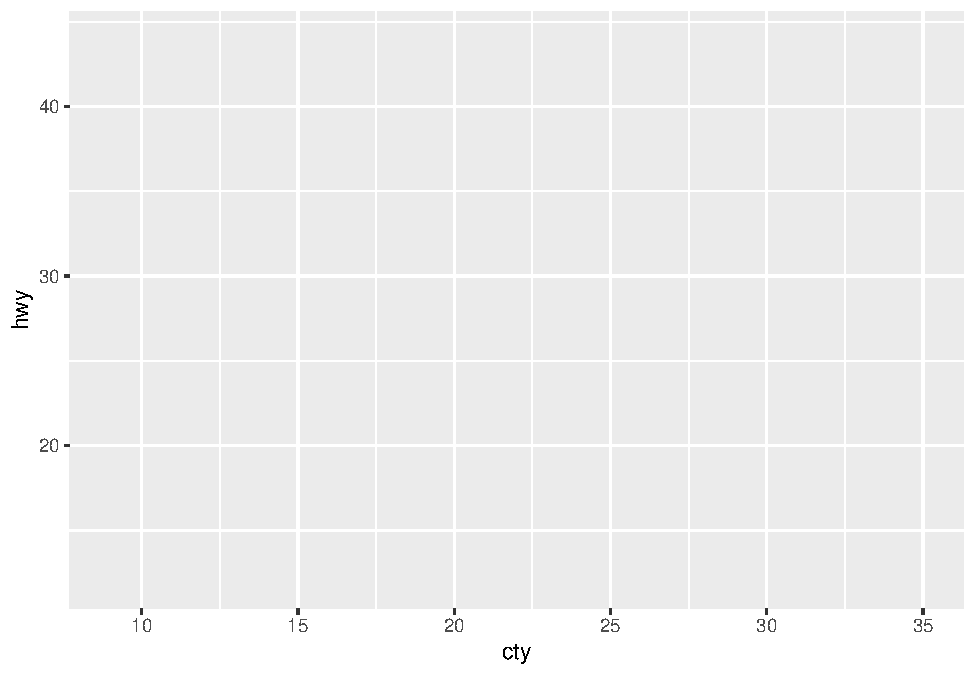
\includegraphics{02_ggplot2_files/figure-latex/unnamed-chunk-3-2.pdf}

\begin{Shaded}
\begin{Highlighting}[]
\CommentTok{\# Alternativas}
\FunctionTok{ggplot}\NormalTok{(dados, }\FunctionTok{aes}\NormalTok{(}\AttributeTok{x =}\NormalTok{ cty, }\AttributeTok{y =}\NormalTok{ hwy)) }\SpecialCharTok{+} 
  \FunctionTok{geom\_point}\NormalTok{()}
\end{Highlighting}
\end{Shaded}

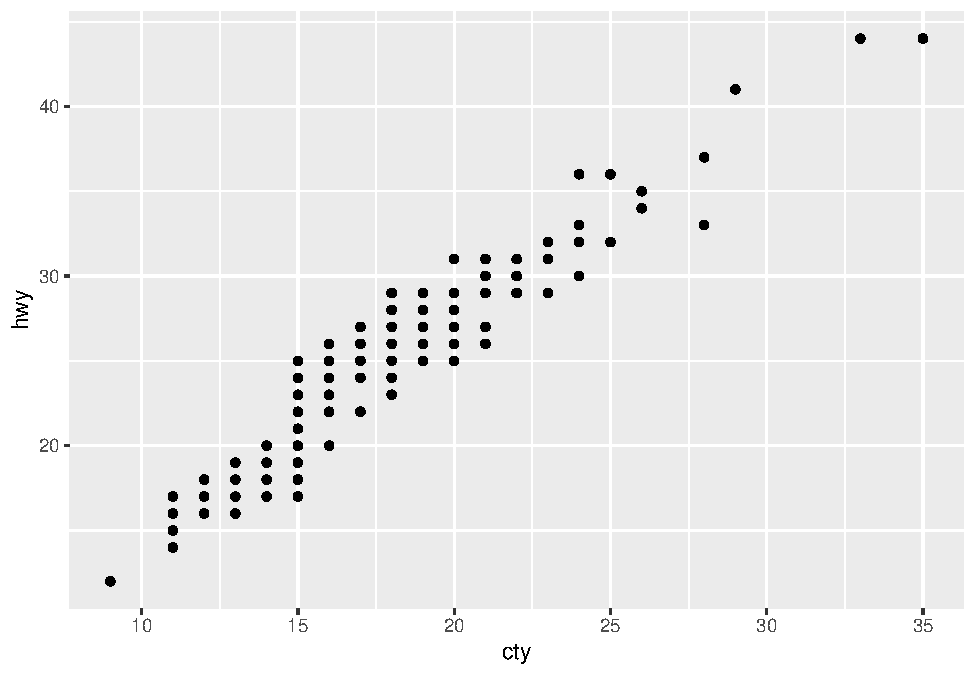
\includegraphics{02_ggplot2_files/figure-latex/unnamed-chunk-3-3.pdf}

\begin{Shaded}
\begin{Highlighting}[]
\FunctionTok{ggplot}\NormalTok{(dados) }\SpecialCharTok{+} 
  \FunctionTok{geom\_point}\NormalTok{(}\FunctionTok{aes}\NormalTok{(}\AttributeTok{x =}\NormalTok{ cty, }\AttributeTok{y =}\NormalTok{ hwy))}
\end{Highlighting}
\end{Shaded}

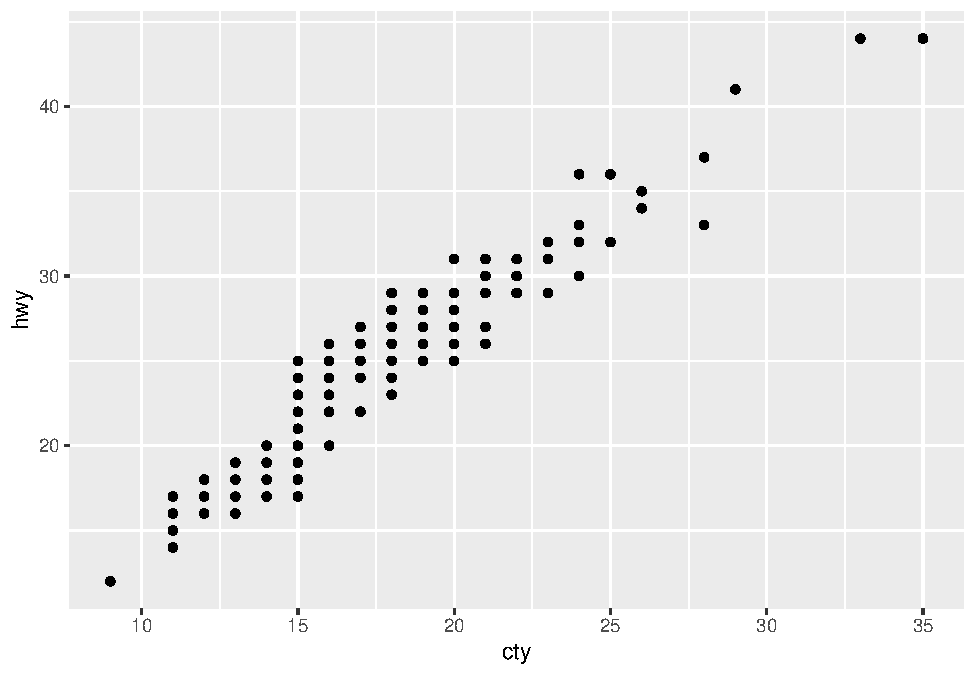
\includegraphics{02_ggplot2_files/figure-latex/unnamed-chunk-3-4.pdf}

\begin{Shaded}
\begin{Highlighting}[]
\FunctionTok{ggplot}\NormalTok{() }\SpecialCharTok{+} 
  \FunctionTok{geom\_point}\NormalTok{(}\AttributeTok{data =}\NormalTok{ dados, }\FunctionTok{aes}\NormalTok{(}\AttributeTok{x =}\NormalTok{ cty, }\AttributeTok{y =}\NormalTok{ hwy))}
\end{Highlighting}
\end{Shaded}

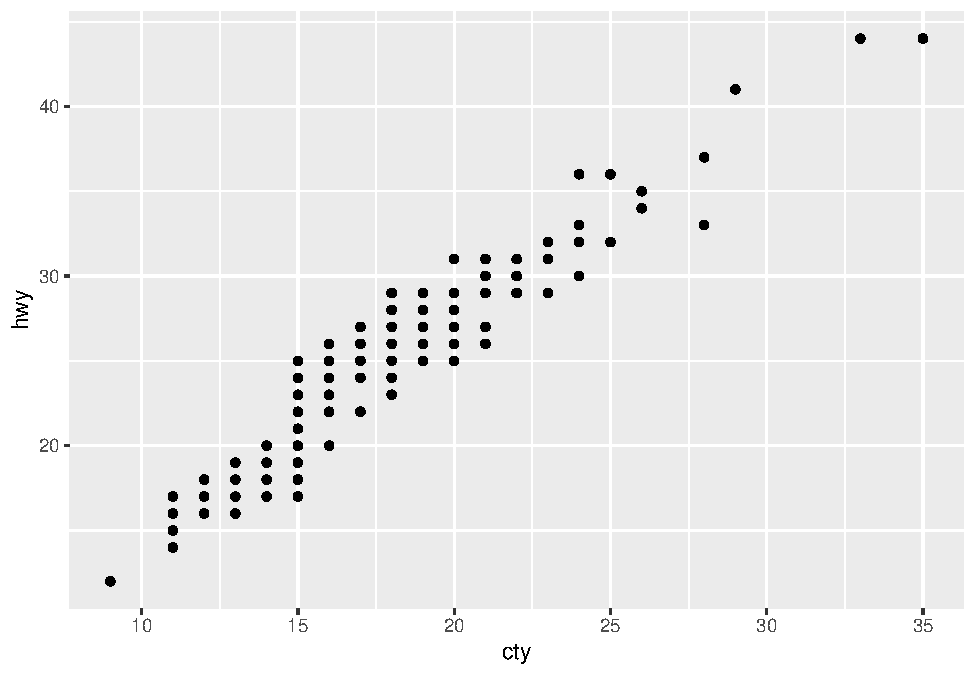
\includegraphics{02_ggplot2_files/figure-latex/unnamed-chunk-3-5.pdf}

\begin{Shaded}
\begin{Highlighting}[]
\CommentTok{\# Fim }

\FunctionTok{ggplot}\NormalTok{(dados, }\FunctionTok{aes}\NormalTok{(}\AttributeTok{x =}\NormalTok{ cty, }\AttributeTok{y =}\NormalTok{ hwy)) }\SpecialCharTok{+} 
  \FunctionTok{geom\_point}\NormalTok{(}\AttributeTok{colour =} \StringTok{"red"}\NormalTok{)}
\end{Highlighting}
\end{Shaded}

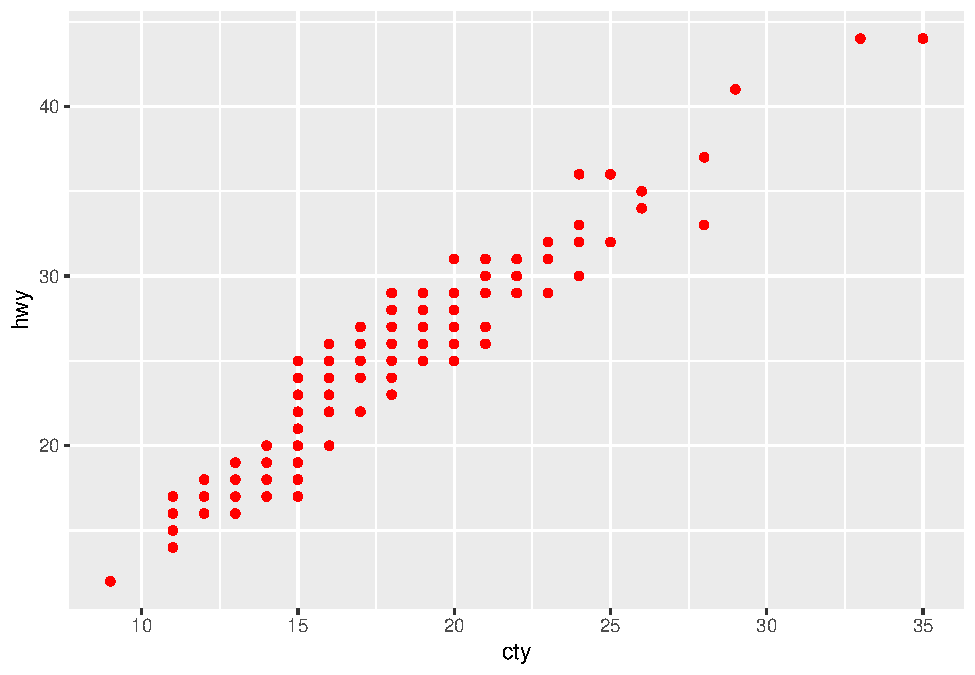
\includegraphics{02_ggplot2_files/figure-latex/unnamed-chunk-3-6.pdf}

\begin{Shaded}
\begin{Highlighting}[]
\FunctionTok{ggplot}\NormalTok{(dados, }\FunctionTok{aes}\NormalTok{(}\AttributeTok{x =}\NormalTok{ cty, }\AttributeTok{y =}\NormalTok{ hwy)) }\SpecialCharTok{+} 
  \FunctionTok{geom\_point}\NormalTok{(}\AttributeTok{colour =} \StringTok{"red"}\NormalTok{, }\AttributeTok{size =} \DecValTok{6}\NormalTok{)}
\end{Highlighting}
\end{Shaded}

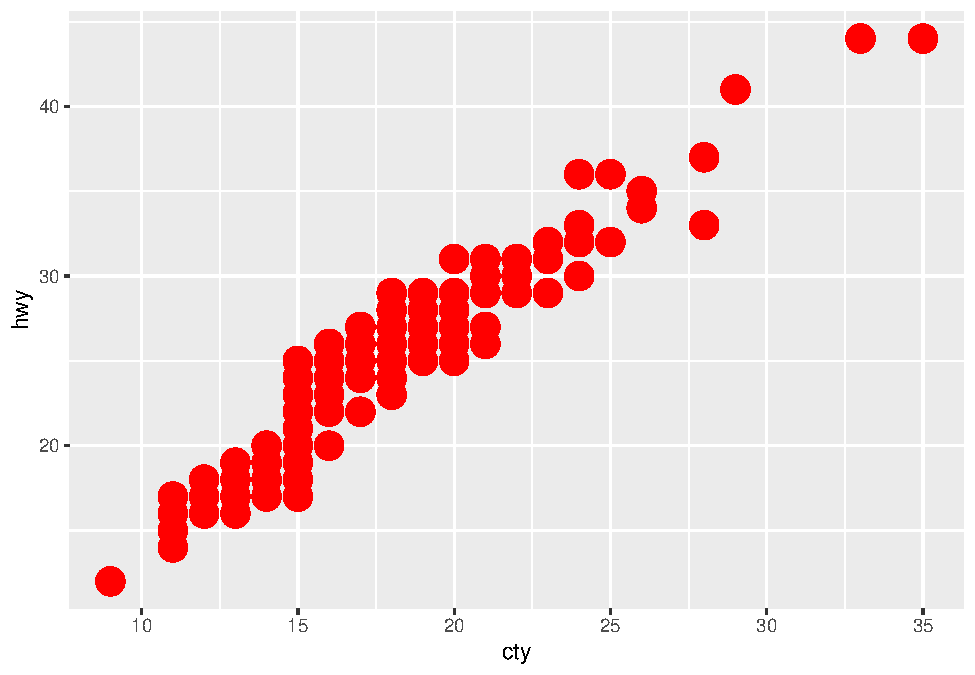
\includegraphics{02_ggplot2_files/figure-latex/unnamed-chunk-3-7.pdf}

\begin{Shaded}
\begin{Highlighting}[]
\FunctionTok{ggplot}\NormalTok{(dados, }\FunctionTok{aes}\NormalTok{(}\AttributeTok{x =}\NormalTok{ cty, }\AttributeTok{y =}\NormalTok{ hwy)) }\SpecialCharTok{+} 
  \FunctionTok{geom\_point}\NormalTok{(}\AttributeTok{colour =} \StringTok{"red"}\NormalTok{, }\AttributeTok{size =} \DecValTok{6}\NormalTok{, }\AttributeTok{shape =} \DecValTok{10}\NormalTok{)}
\end{Highlighting}
\end{Shaded}

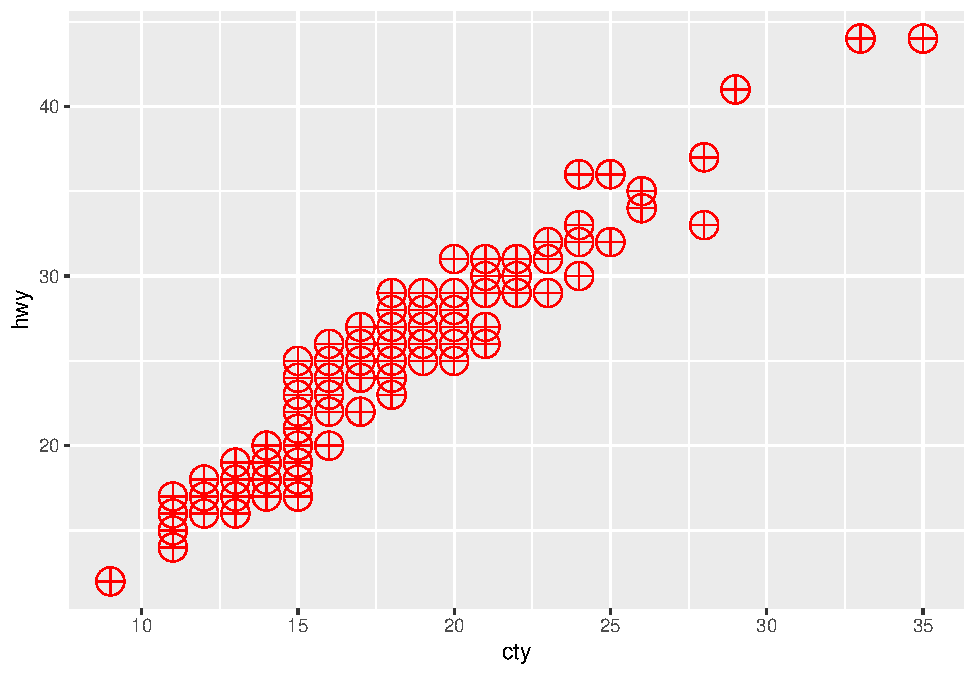
\includegraphics{02_ggplot2_files/figure-latex/unnamed-chunk-3-8.pdf}

\begin{Shaded}
\begin{Highlighting}[]
\CommentTok{\# Alternativa}
\FunctionTok{ggplot}\NormalTok{(dados, }\FunctionTok{aes}\NormalTok{(}\AttributeTok{x =}\NormalTok{ cty, }\AttributeTok{y =}\NormalTok{ hwy)) }\SpecialCharTok{+} 
  \FunctionTok{geom\_point}\NormalTok{(}\AttributeTok{colour =} \StringTok{"red"}\NormalTok{, }\AttributeTok{size =} \DecValTok{6}\NormalTok{, }\AttributeTok{shape =} \StringTok{"circle plus"}\NormalTok{)}
\end{Highlighting}
\end{Shaded}

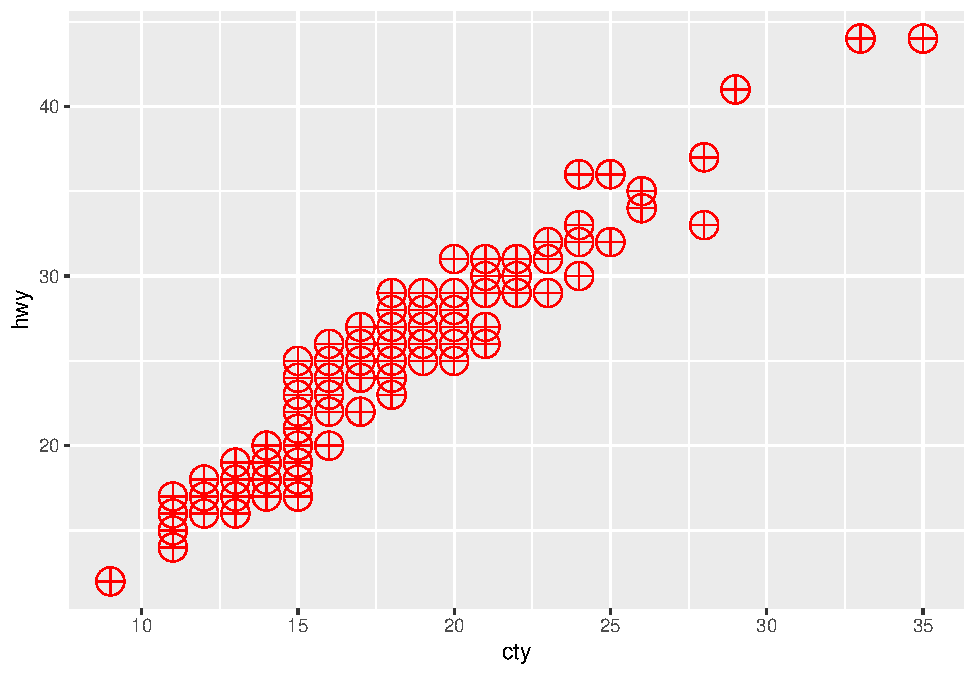
\includegraphics{02_ggplot2_files/figure-latex/unnamed-chunk-3-9.pdf}

\begin{Shaded}
\begin{Highlighting}[]
\FunctionTok{ggplot}\NormalTok{(dados, }\FunctionTok{aes}\NormalTok{(}\AttributeTok{x =}\NormalTok{ cty, }\AttributeTok{y =}\NormalTok{ hwy)) }\SpecialCharTok{+} 
  \FunctionTok{geom\_point}\NormalTok{(}\AttributeTok{colour =} \StringTok{"red"}\NormalTok{, }\AttributeTok{size =} \DecValTok{6}\NormalTok{, }\AttributeTok{shape =} \DecValTok{10}\NormalTok{)}\SpecialCharTok{+}
  \FunctionTok{labs}\NormalTok{(}\AttributeTok{x =} \StringTok{"cty (city miles per gallon hwy)"}\NormalTok{, }
       \AttributeTok{y =} \StringTok{"hwy (highway miles per gallon)"}\NormalTok{, }
       \AttributeTok{title =} \StringTok{"Pensar em algum título..."}\NormalTok{, }
       \AttributeTok{subtitle =} \StringTok{"Escrever alguma coisa"}\NormalTok{)}
\end{Highlighting}
\end{Shaded}

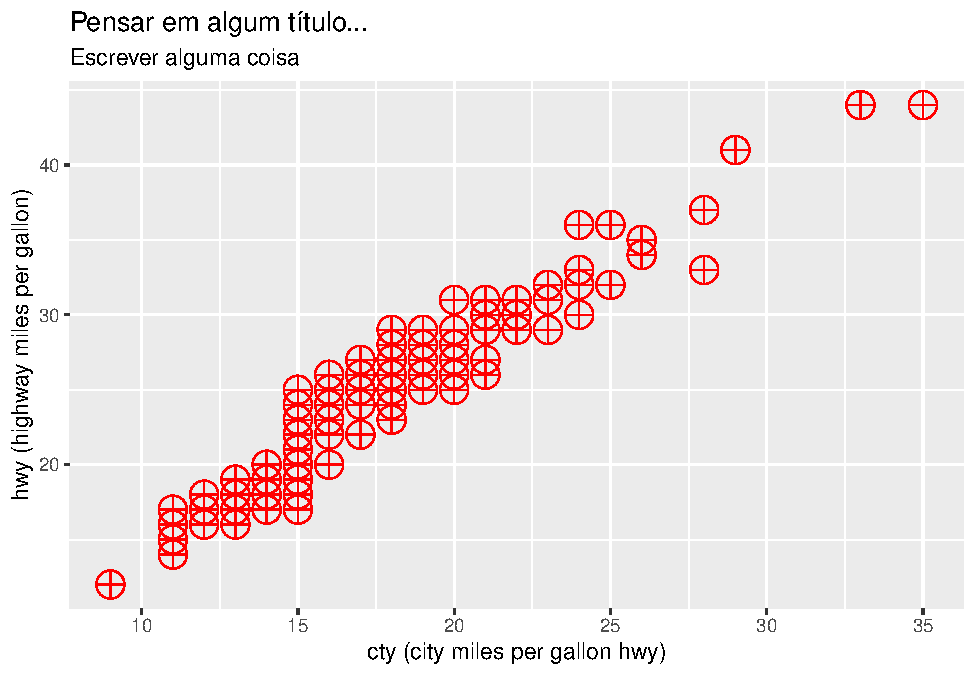
\includegraphics{02_ggplot2_files/figure-latex/unnamed-chunk-3-10.pdf}

\hypertarget{mais-detalhes-sobre-geom_point}{%
\subsection{Mais detalhes sobre geom\_point}\label{mais-detalhes-sobre-geom_point}}

\begin{quote}
geom\_point() understands the following aesthetics (required aesthetics are in bold):
\end{quote}

\begin{itemize}
\item
  x
\item
  y
\item
  alpha
\item
  colour
\item
  fill
\item
  group
\item
  shape
\item
  size
\item
  stroke
\end{itemize}

\begin{Shaded}
\begin{Highlighting}[]
\FunctionTok{ggplot}\NormalTok{(dados, }\FunctionTok{aes}\NormalTok{(}\AttributeTok{x =}\NormalTok{ cty, }\AttributeTok{y =}\NormalTok{ hwy)) }\SpecialCharTok{+} 
  \FunctionTok{geom\_point}\NormalTok{()}
\end{Highlighting}
\end{Shaded}

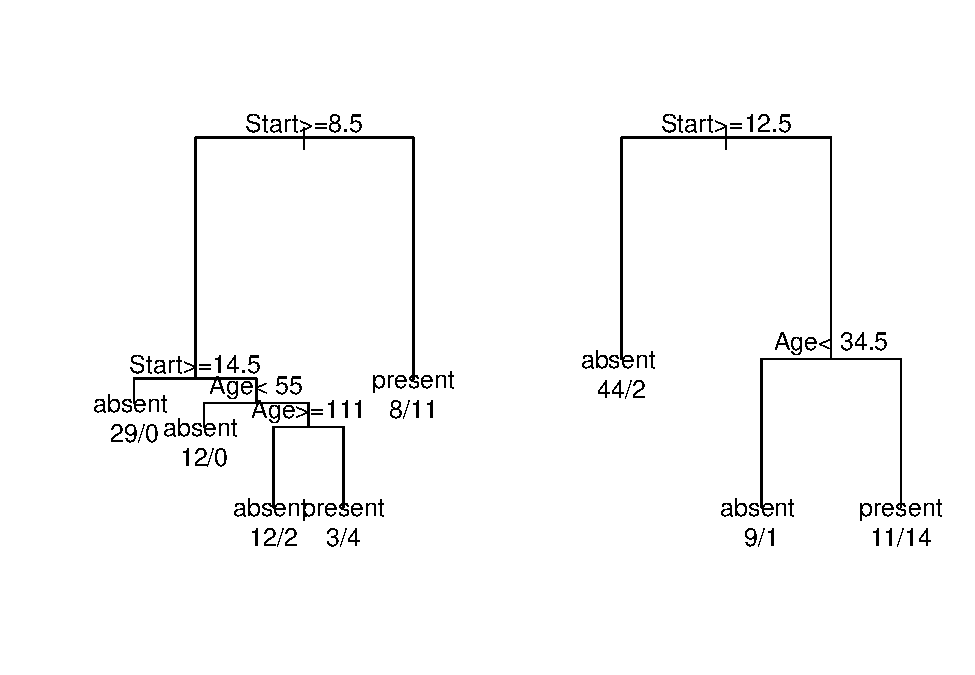
\includegraphics{02_ggplot2_files/figure-latex/unnamed-chunk-4-1.pdf}

\begin{Shaded}
\begin{Highlighting}[]
\FunctionTok{ggplot}\NormalTok{(dados, }\FunctionTok{aes}\NormalTok{(}\AttributeTok{x =}\NormalTok{ cty, }\AttributeTok{y =}\NormalTok{ hwy, }\AttributeTok{col =} \FunctionTok{factor}\NormalTok{(year))) }\SpecialCharTok{+} 
  \FunctionTok{geom\_point}\NormalTok{() }\SpecialCharTok{+} 
  \FunctionTok{labs}\NormalTok{(}\AttributeTok{col =} \StringTok{"year"}\NormalTok{)}
\end{Highlighting}
\end{Shaded}

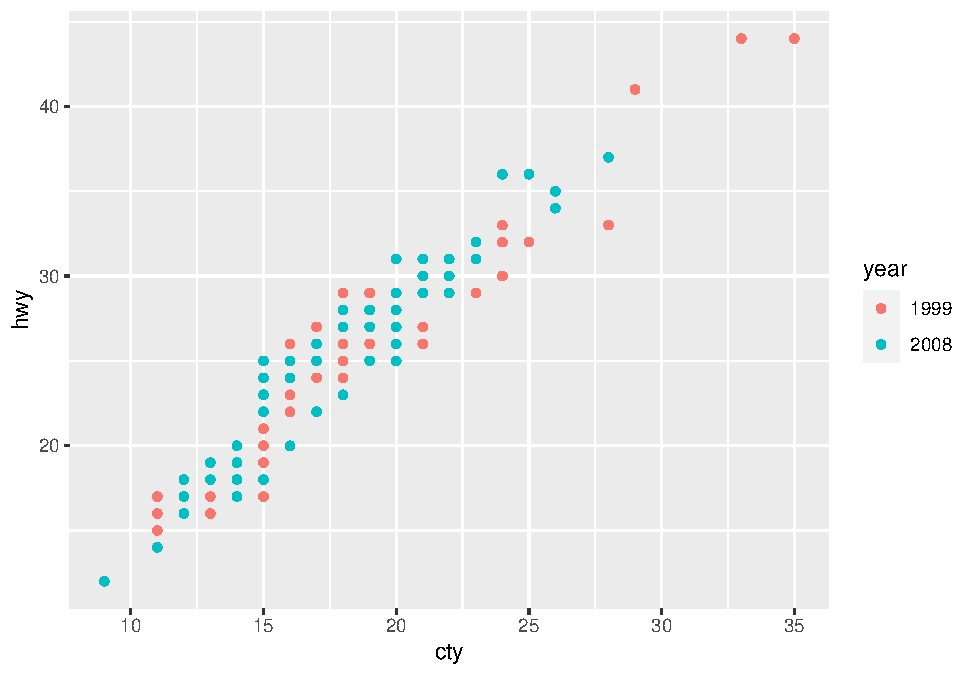
\includegraphics{02_ggplot2_files/figure-latex/unnamed-chunk-4-2.pdf}

\begin{Shaded}
\begin{Highlighting}[]
\CommentTok{\# Alternativa}
\FunctionTok{ggplot}\NormalTok{(dados, }\FunctionTok{aes}\NormalTok{(}\AttributeTok{x =}\NormalTok{ cty, }\AttributeTok{y =}\NormalTok{ hwy, }\AttributeTok{col =} \FunctionTok{factor}\NormalTok{(class))) }\SpecialCharTok{+} 
  \FunctionTok{geom\_point}\NormalTok{() }\SpecialCharTok{+} 
  \FunctionTok{labs}\NormalTok{(}\AttributeTok{col =} \StringTok{"class"}\NormalTok{)}\SpecialCharTok{+}
  \FunctionTok{scale\_color\_brewer}\NormalTok{(}\AttributeTok{type =} \StringTok{"qual"}\NormalTok{)}
\end{Highlighting}
\end{Shaded}

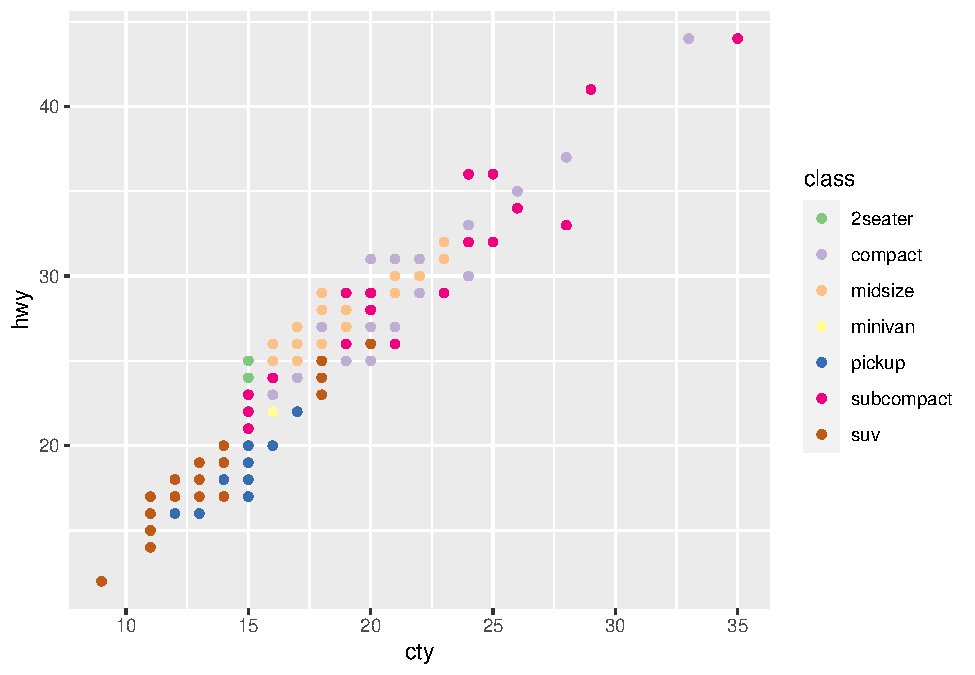
\includegraphics{02_ggplot2_files/figure-latex/unnamed-chunk-4-3.pdf}

\begin{Shaded}
\begin{Highlighting}[]
\FunctionTok{ggplot}\NormalTok{(dados, }\FunctionTok{aes}\NormalTok{(}\AttributeTok{x =}\NormalTok{ cty, }\AttributeTok{y =}\NormalTok{ hwy, }\AttributeTok{col =} \FunctionTok{factor}\NormalTok{(class))) }\SpecialCharTok{+} 
  \FunctionTok{geom\_point}\NormalTok{() }\SpecialCharTok{+} 
  \FunctionTok{labs}\NormalTok{(}\AttributeTok{col =} \StringTok{"class"}\NormalTok{)}\SpecialCharTok{+}
  \FunctionTok{scale\_color\_brewer}\NormalTok{(}\AttributeTok{type =} \StringTok{"div"}\NormalTok{)}
\end{Highlighting}
\end{Shaded}

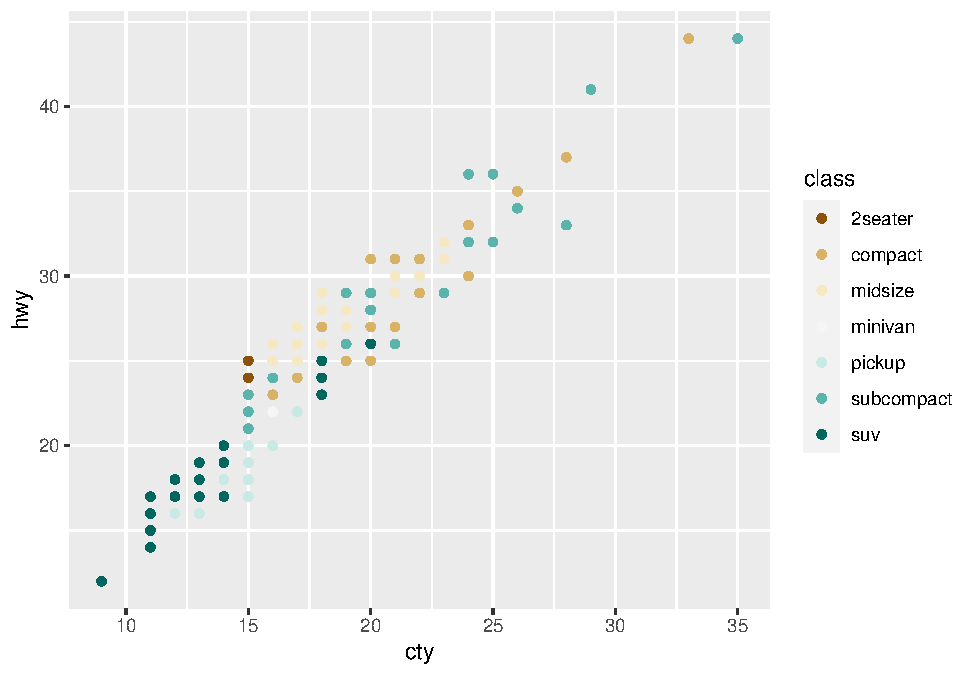
\includegraphics{02_ggplot2_files/figure-latex/unnamed-chunk-4-4.pdf}

\begin{Shaded}
\begin{Highlighting}[]
\FunctionTok{ggplot}\NormalTok{(dados, }\FunctionTok{aes}\NormalTok{(}\AttributeTok{x =}\NormalTok{ cty, }\AttributeTok{y =}\NormalTok{ hwy, }\AttributeTok{col =} \FunctionTok{factor}\NormalTok{(class))) }\SpecialCharTok{+} 
  \FunctionTok{geom\_point}\NormalTok{() }\SpecialCharTok{+} 
  \FunctionTok{labs}\NormalTok{(}\AttributeTok{col =} \StringTok{"class"}\NormalTok{)}\SpecialCharTok{+}
  \FunctionTok{scale\_color\_brewer}\NormalTok{(}\AttributeTok{palette =} \StringTok{"Set1"}\NormalTok{, }\AttributeTok{name =} \StringTok{"Tipo de carro"}\NormalTok{)}\SpecialCharTok{+}
  \FunctionTok{scale\_y\_continuous}\NormalTok{(}\AttributeTok{breaks =} \FunctionTok{seq}\NormalTok{(}\DecValTok{10}\NormalTok{,}\DecValTok{60}\NormalTok{,}\DecValTok{3}\NormalTok{))}\SpecialCharTok{+}
  \FunctionTok{scale\_x\_continuous}\NormalTok{(}\AttributeTok{breaks =} \FunctionTok{seq}\NormalTok{(}\DecValTok{10}\NormalTok{,}\DecValTok{40}\NormalTok{,}\DecValTok{3}\NormalTok{))}\SpecialCharTok{+}
  \FunctionTok{theme\_minimal}\NormalTok{()}
\end{Highlighting}
\end{Shaded}

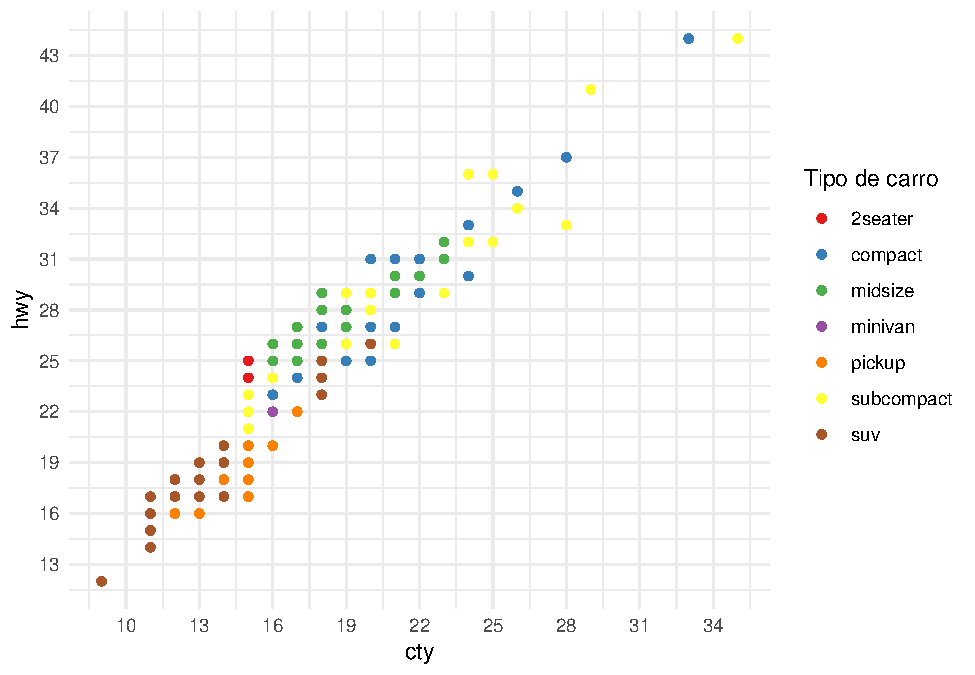
\includegraphics{02_ggplot2_files/figure-latex/unnamed-chunk-4-5.pdf}

\begin{Shaded}
\begin{Highlighting}[]
\FunctionTok{ggplot}\NormalTok{(dados, }\FunctionTok{aes}\NormalTok{(}\AttributeTok{x =}\NormalTok{ cty, }\AttributeTok{y =}\NormalTok{ hwy, }\AttributeTok{alpha =} \FunctionTok{factor}\NormalTok{(year))) }\SpecialCharTok{+} 
  \FunctionTok{geom\_point}\NormalTok{() }\SpecialCharTok{+} 
  \FunctionTok{labs}\NormalTok{(}\AttributeTok{alpha =} \StringTok{"year"}\NormalTok{)}
\end{Highlighting}
\end{Shaded}

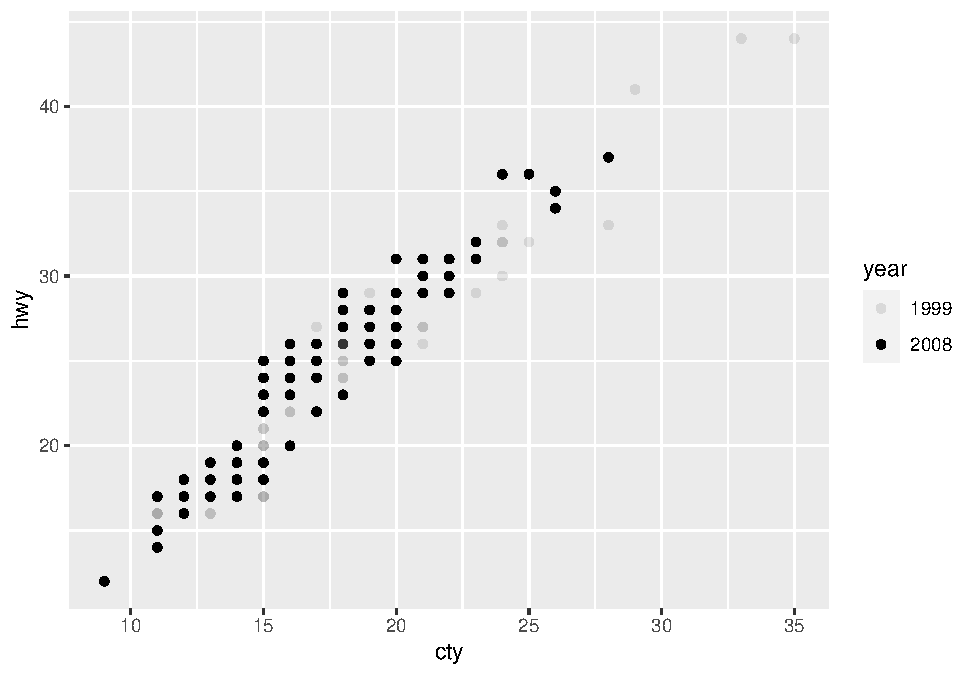
\includegraphics{02_ggplot2_files/figure-latex/unnamed-chunk-4-6.pdf}

\begin{Shaded}
\begin{Highlighting}[]
\FunctionTok{ggplot}\NormalTok{(dados, }\FunctionTok{aes}\NormalTok{(}\AttributeTok{x =}\NormalTok{ cty, }\AttributeTok{y =}\NormalTok{ hwy, }\AttributeTok{size =} \FunctionTok{factor}\NormalTok{(year))) }\SpecialCharTok{+} 
  \FunctionTok{geom\_point}\NormalTok{() }\SpecialCharTok{+} 
  \FunctionTok{labs}\NormalTok{(}\AttributeTok{size =} \StringTok{"year"}\NormalTok{)}
\end{Highlighting}
\end{Shaded}

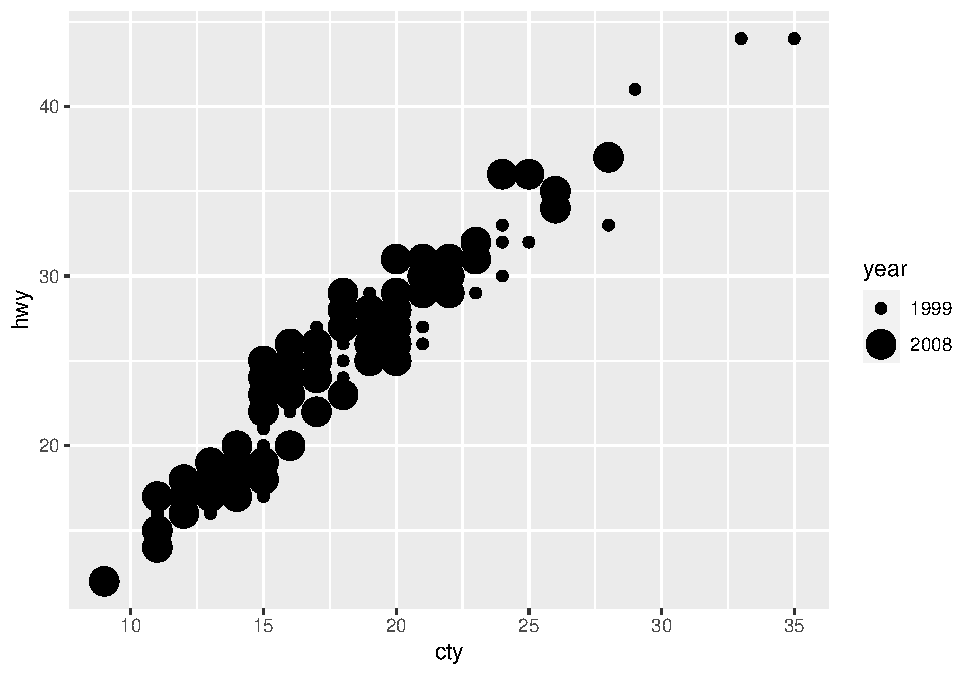
\includegraphics{02_ggplot2_files/figure-latex/unnamed-chunk-4-7.pdf}

\begin{Shaded}
\begin{Highlighting}[]
\CommentTok{\# Alternativa}
\FunctionTok{ggplot}\NormalTok{(dados, }\FunctionTok{aes}\NormalTok{(}\AttributeTok{x =}\NormalTok{ cty, }\AttributeTok{y =}\NormalTok{ hwy, }\AttributeTok{col =}\NormalTok{ cty }\SpecialCharTok{\textless{}=} \DecValTok{20}\NormalTok{)) }\SpecialCharTok{+} 
  \FunctionTok{geom\_point}\NormalTok{() }\SpecialCharTok{+} 
  \FunctionTok{geom\_vline}\NormalTok{(}\AttributeTok{xintercept =} \DecValTok{20}\NormalTok{)}\SpecialCharTok{+}
  \FunctionTok{labs}\NormalTok{(}\AttributeTok{col =} \StringTok{"year"}\NormalTok{)}
\end{Highlighting}
\end{Shaded}

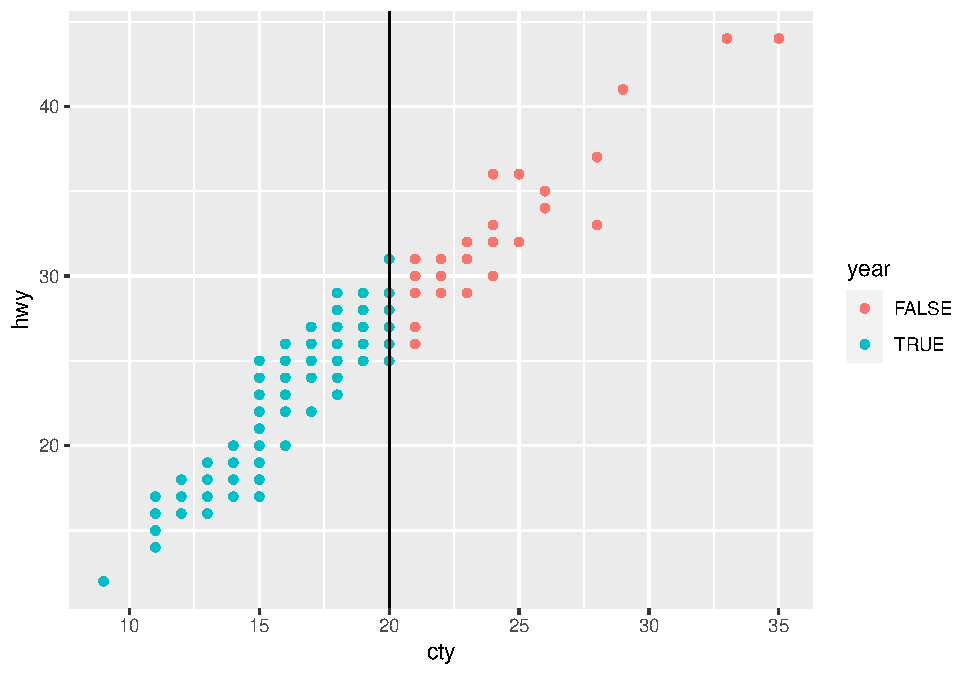
\includegraphics{02_ggplot2_files/figure-latex/unnamed-chunk-4-8.pdf}

\begin{Shaded}
\begin{Highlighting}[]
\CommentTok{\# Erro comum}
\FunctionTok{ggplot}\NormalTok{(dados, }\FunctionTok{aes}\NormalTok{(}\AttributeTok{x =}\NormalTok{ cty, }\AttributeTok{y =}\NormalTok{ hwy, }\AttributeTok{col =} \StringTok{"red"}\NormalTok{)) }\SpecialCharTok{+} 
  \FunctionTok{geom\_point}\NormalTok{()}\SpecialCharTok{+}
  \FunctionTok{labs}\NormalTok{(}\AttributeTok{col =} \StringTok{"year"}\NormalTok{)}
\end{Highlighting}
\end{Shaded}

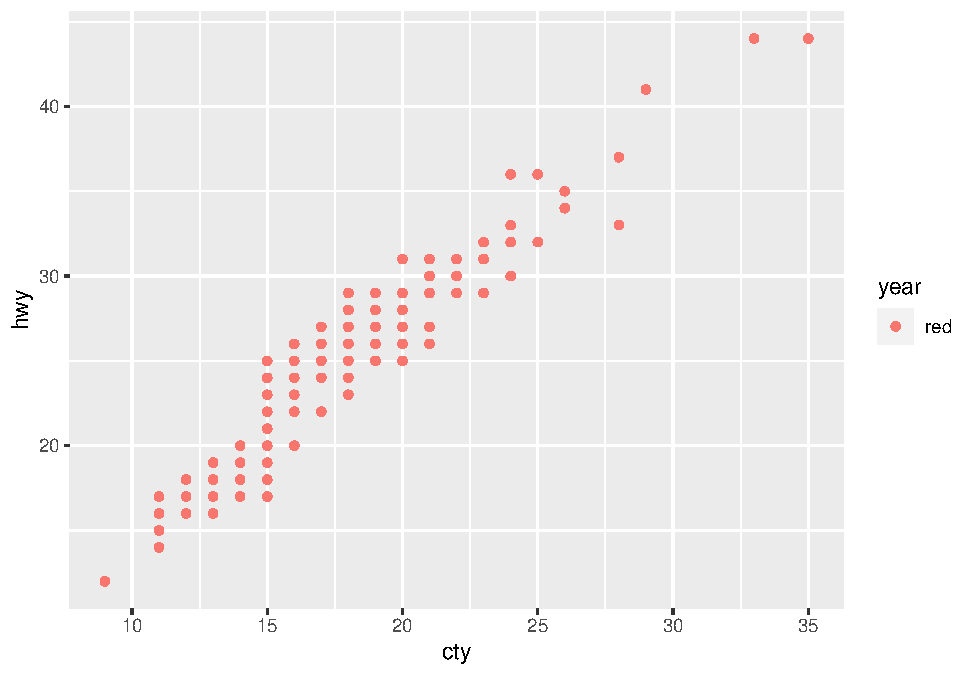
\includegraphics{02_ggplot2_files/figure-latex/unnamed-chunk-4-9.pdf}

\begin{Shaded}
\begin{Highlighting}[]
\FunctionTok{ggplot}\NormalTok{(dados, }\FunctionTok{aes}\NormalTok{(}\AttributeTok{x =}\NormalTok{ cty, }\AttributeTok{y =}\NormalTok{ hwy)) }\SpecialCharTok{+} 
  \FunctionTok{geom\_point}\NormalTok{(}\AttributeTok{col =} \StringTok{"red"}\NormalTok{)}\SpecialCharTok{+}
  \FunctionTok{labs}\NormalTok{(}\AttributeTok{col =} \StringTok{"year"}\NormalTok{)}
\end{Highlighting}
\end{Shaded}

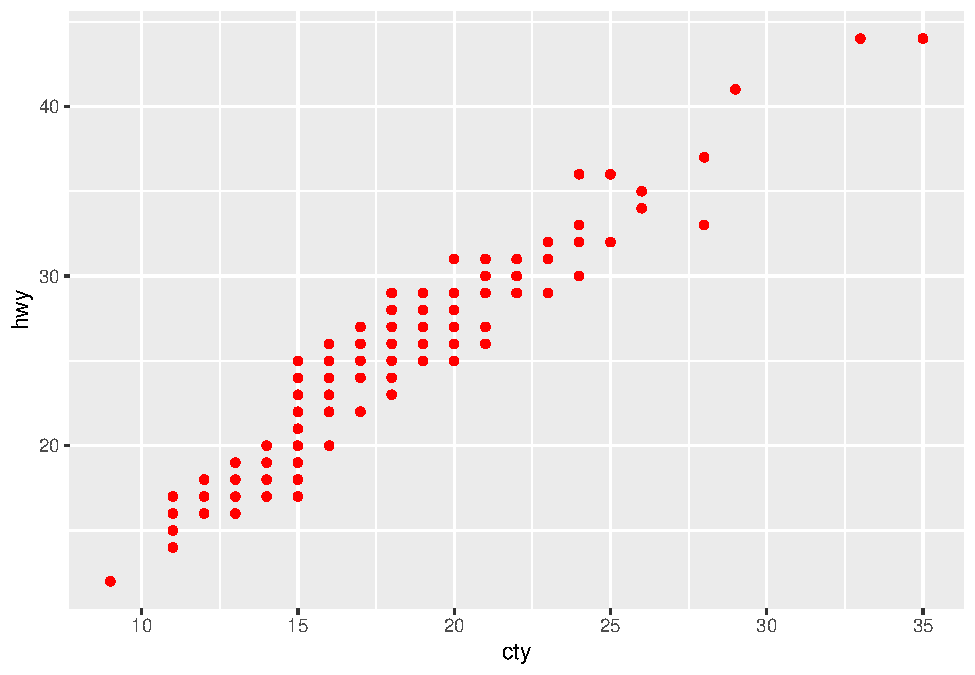
\includegraphics{02_ggplot2_files/figure-latex/unnamed-chunk-4-10.pdf}

\begin{Shaded}
\begin{Highlighting}[]
\CommentTok{\# Fim  Erro comum}

\FunctionTok{ggplot}\NormalTok{(dados, }\FunctionTok{aes}\NormalTok{(}\AttributeTok{x =}\NormalTok{ cty, }\AttributeTok{y =}\NormalTok{ hwy, }\AttributeTok{shape =} \FunctionTok{factor}\NormalTok{(year))) }\SpecialCharTok{+} 
  \FunctionTok{geom\_point}\NormalTok{(}\AttributeTok{col =} \StringTok{"red"}\NormalTok{) }\SpecialCharTok{+} 
  \FunctionTok{labs}\NormalTok{(}\AttributeTok{shape =} \StringTok{"year"}\NormalTok{)}
\end{Highlighting}
\end{Shaded}

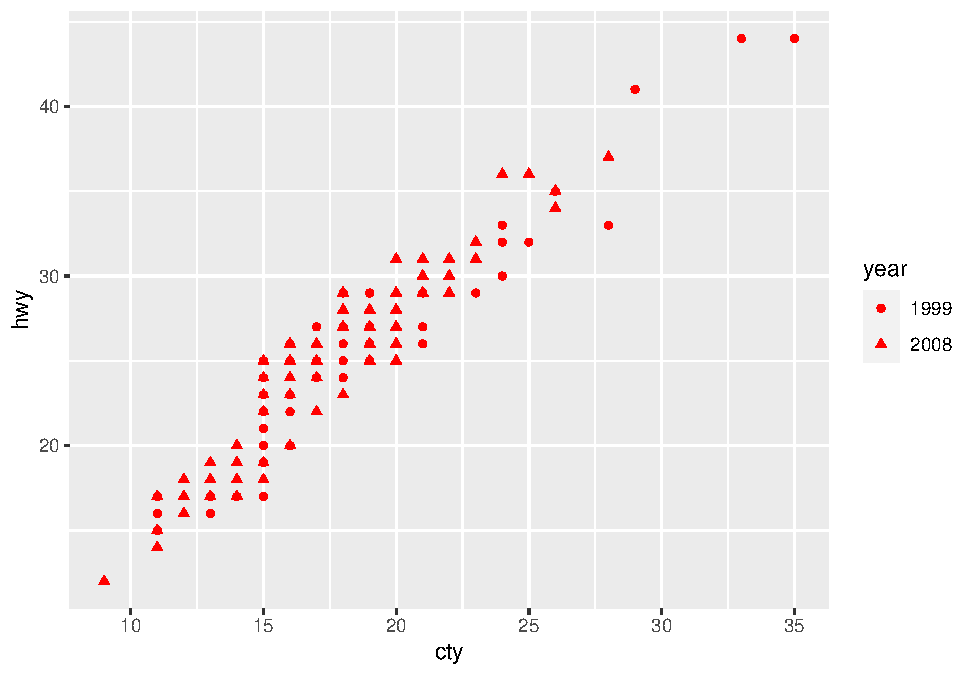
\includegraphics{02_ggplot2_files/figure-latex/unnamed-chunk-4-11.pdf}

\begin{Shaded}
\begin{Highlighting}[]
\FunctionTok{ggplot}\NormalTok{(dados, }\FunctionTok{aes}\NormalTok{(}\AttributeTok{x =}\NormalTok{ cty, }\AttributeTok{y =}\NormalTok{ hwy, }\AttributeTok{size =}\NormalTok{ class)) }\SpecialCharTok{+} 
  \FunctionTok{geom\_point}\NormalTok{() }\SpecialCharTok{+} 
  \FunctionTok{labs}\NormalTok{(}\AttributeTok{size =} \StringTok{"class"}\NormalTok{)}
\end{Highlighting}
\end{Shaded}

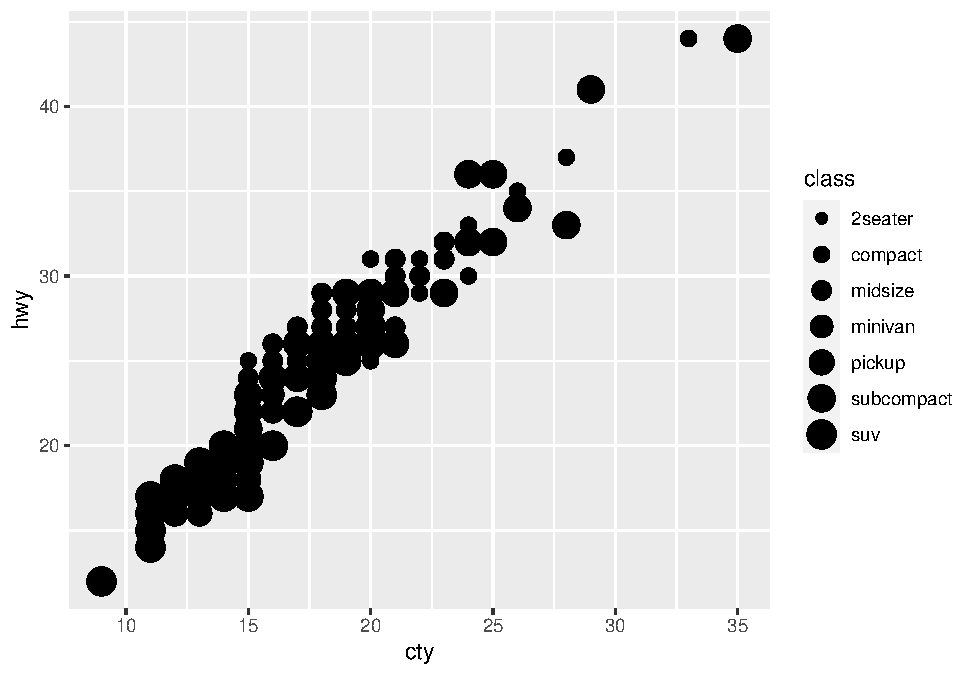
\includegraphics{02_ggplot2_files/figure-latex/unnamed-chunk-4-12.pdf}

\begin{Shaded}
\begin{Highlighting}[]
\FunctionTok{ggplot}\NormalTok{(dados, }\FunctionTok{aes}\NormalTok{(}\AttributeTok{x =}\NormalTok{ cty, }\AttributeTok{y =}\NormalTok{ hwy, }
                  \AttributeTok{size =}\NormalTok{ class, }
                  \AttributeTok{col =}\NormalTok{ class)) }\SpecialCharTok{+} 
  \FunctionTok{geom\_point}\NormalTok{() }\SpecialCharTok{+} 
  \FunctionTok{guides}\NormalTok{(}\AttributeTok{colour =} \FunctionTok{guide\_legend}\NormalTok{(}\StringTok{"Tipo de carro (color)"}\NormalTok{),}
         \AttributeTok{size =} \FunctionTok{guide\_legend}\NormalTok{(}\StringTok{"Tipo de carro (size)"}\NormalTok{))}
\end{Highlighting}
\end{Shaded}

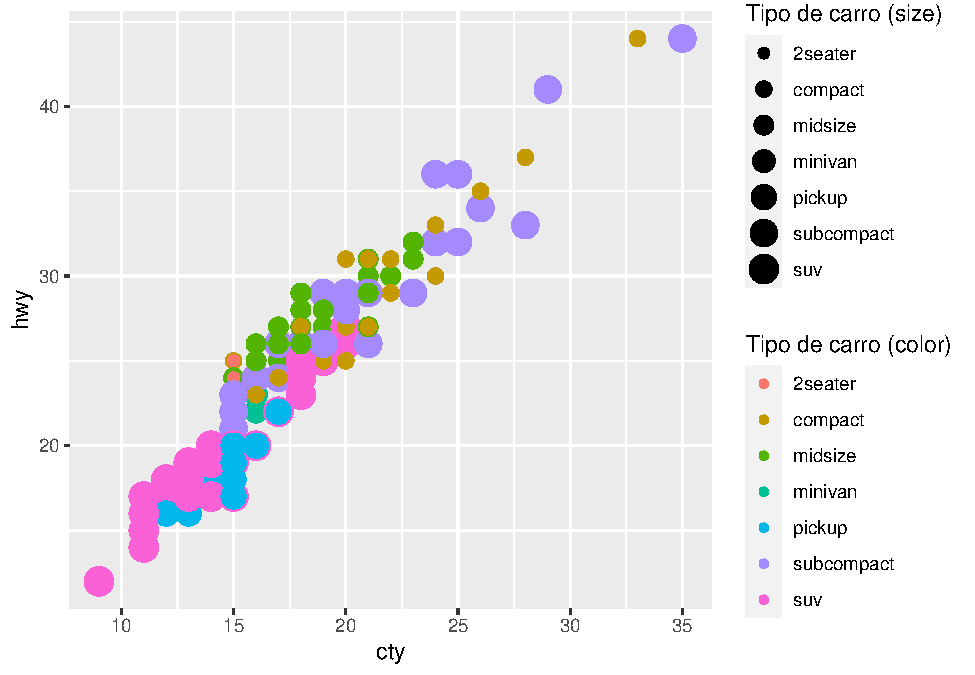
\includegraphics{02_ggplot2_files/figure-latex/unnamed-chunk-4-13.pdf}

\begin{Shaded}
\begin{Highlighting}[]
\FunctionTok{ggplot}\NormalTok{(dados, }\FunctionTok{aes}\NormalTok{(}\AttributeTok{x =}\NormalTok{ cty, }\AttributeTok{y =}\NormalTok{ hwy, }
                  \AttributeTok{size =}\NormalTok{ class, }
                  \AttributeTok{col =}\NormalTok{ class)) }\SpecialCharTok{+} 
  \FunctionTok{geom\_point}\NormalTok{() }\SpecialCharTok{+} 
  \FunctionTok{labs}\NormalTok{(}\AttributeTok{col =} \StringTok{"Tipo de Carro"}\NormalTok{, }\AttributeTok{size =} \StringTok{"Tipo de Carro"}\NormalTok{)}\SpecialCharTok{+}
  \FunctionTok{guides}\NormalTok{(}\AttributeTok{col =} \StringTok{"legend"}\NormalTok{)}
\end{Highlighting}
\end{Shaded}

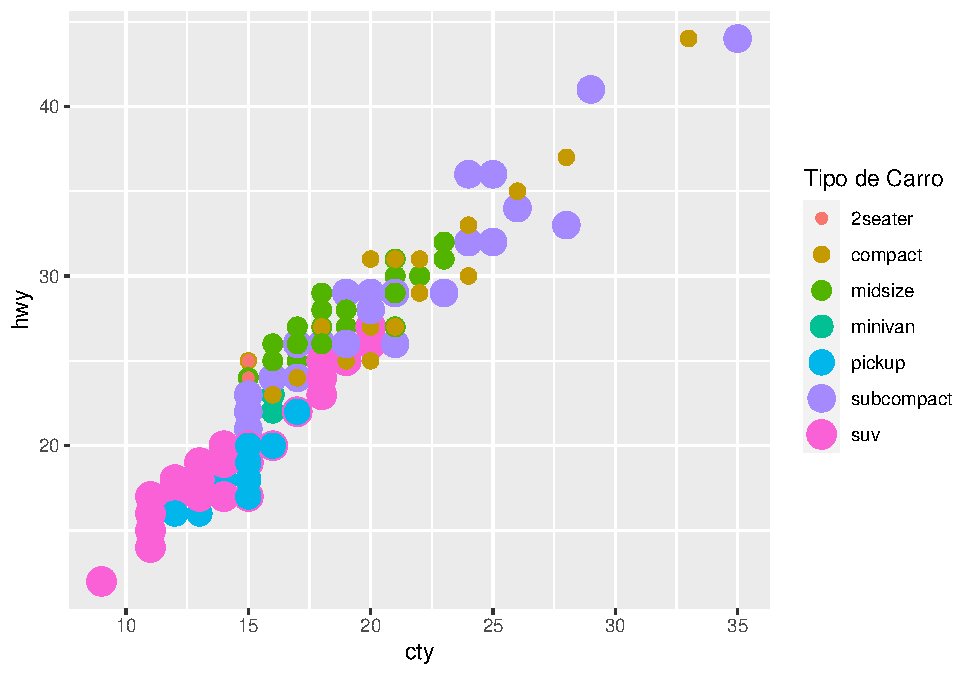
\includegraphics{02_ggplot2_files/figure-latex/unnamed-chunk-4-14.pdf}

\hypertarget{smooth-boxplot-histogram}{%
\section{smooth, boxplot, histogram}\label{smooth-boxplot-histogram}}

\begin{Shaded}
\begin{Highlighting}[]
\NormalTok{v1}\OtherTok{\textless{}{-}} \FunctionTok{ggplot}\NormalTok{(dados, }\FunctionTok{aes}\NormalTok{(}\AttributeTok{x =}\NormalTok{ cty, }\AttributeTok{y =}\NormalTok{ hwy)) }\SpecialCharTok{+} 
  \FunctionTok{geom\_point}\NormalTok{(}\AttributeTok{col =} \StringTok{"blue"}\NormalTok{)}\SpecialCharTok{+}
  \FunctionTok{geom\_smooth}\NormalTok{(}\AttributeTok{method =}\NormalTok{ mgcv}\SpecialCharTok{::}\NormalTok{gam,}
              \AttributeTok{formula =}\NormalTok{ y }\SpecialCharTok{\textasciitilde{}} \FunctionTok{s}\NormalTok{(x, }\AttributeTok{bs =} \StringTok{"cs"}\NormalTok{) ,}
              \AttributeTok{col =} \StringTok{"red"}\NormalTok{, }
              \AttributeTok{se =} \ConstantTok{FALSE}\NormalTok{)}
\NormalTok{v1}
\end{Highlighting}
\end{Shaded}

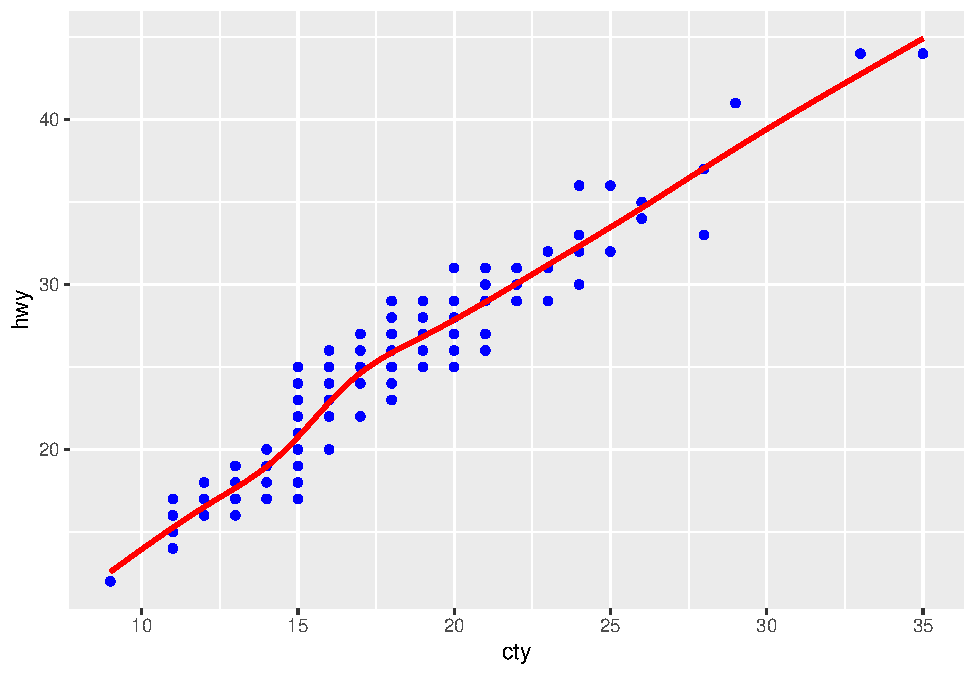
\includegraphics{02_ggplot2_files/figure-latex/unnamed-chunk-5-1.pdf}

\begin{Shaded}
\begin{Highlighting}[]
\NormalTok{v2 }\OtherTok{\textless{}{-}} \FunctionTok{ggplot}\NormalTok{(dados, }\FunctionTok{aes}\NormalTok{(}\AttributeTok{x =}\NormalTok{ cty)) }\SpecialCharTok{+} 
  \FunctionTok{geom\_boxplot}\NormalTok{(}\AttributeTok{fill =} \StringTok{"red"}\NormalTok{)}
\NormalTok{v2}
\end{Highlighting}
\end{Shaded}

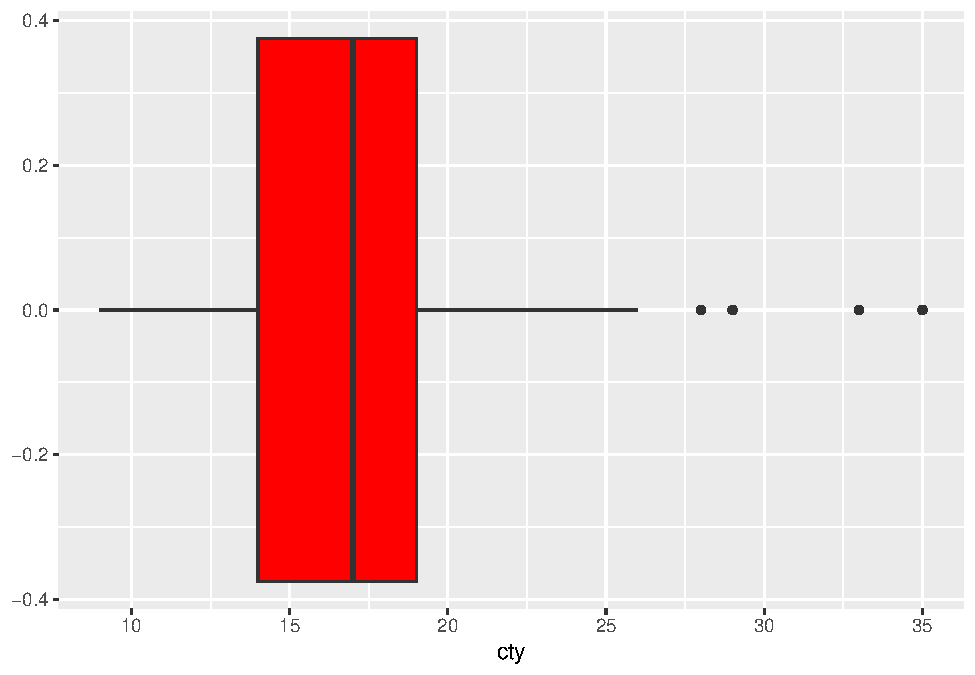
\includegraphics{02_ggplot2_files/figure-latex/unnamed-chunk-5-2.pdf}

\begin{Shaded}
\begin{Highlighting}[]
\NormalTok{v3 }\OtherTok{\textless{}{-}} \FunctionTok{ggplot}\NormalTok{(dados, }\FunctionTok{aes}\NormalTok{(}\AttributeTok{x =}\NormalTok{ cty)) }\SpecialCharTok{+} 
  \FunctionTok{geom\_histogram}\NormalTok{(}\AttributeTok{bins =} \DecValTok{10}\NormalTok{, }\AttributeTok{fill =} \StringTok{"red"}\NormalTok{, }\AttributeTok{col =} \StringTok{"blue"}\NormalTok{, }\AttributeTok{lwd=}\DecValTok{2}\NormalTok{)}
\NormalTok{v3}
\end{Highlighting}
\end{Shaded}

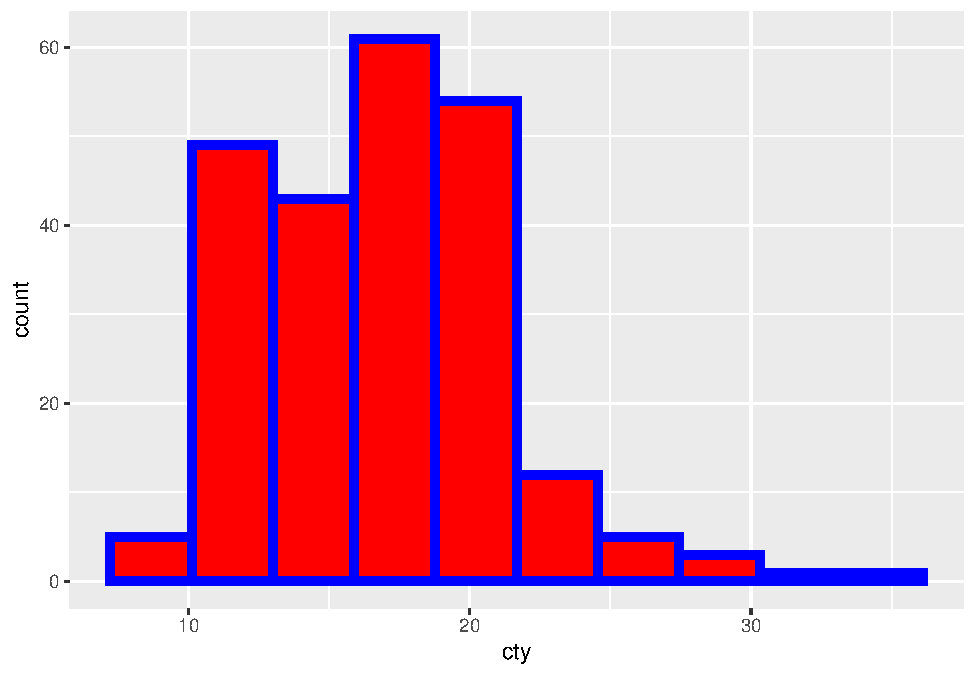
\includegraphics{02_ggplot2_files/figure-latex/unnamed-chunk-5-3.pdf}

\begin{Shaded}
\begin{Highlighting}[]
\NormalTok{v4}\OtherTok{\textless{}{-}} \FunctionTok{ggplot}\NormalTok{(dados, }\FunctionTok{aes}\NormalTok{(}\AttributeTok{x =}\NormalTok{ cty)) }\SpecialCharTok{+} 
  \FunctionTok{geom\_histogram}\NormalTok{(}\FunctionTok{aes}\NormalTok{(}\AttributeTok{y =} \FunctionTok{after\_stat}\NormalTok{(density)),}
                 \AttributeTok{bins =} \DecValTok{10}\NormalTok{, }\AttributeTok{fill =} \StringTok{"yellow"}\NormalTok{, }\AttributeTok{col =} \StringTok{"red"}\NormalTok{) }\SpecialCharTok{+}
  \FunctionTok{geom\_density}\NormalTok{(}\AttributeTok{col =} \StringTok{"blue"}\NormalTok{, }\AttributeTok{lwd =}\DecValTok{3}\NormalTok{)}
\NormalTok{v4}
\end{Highlighting}
\end{Shaded}

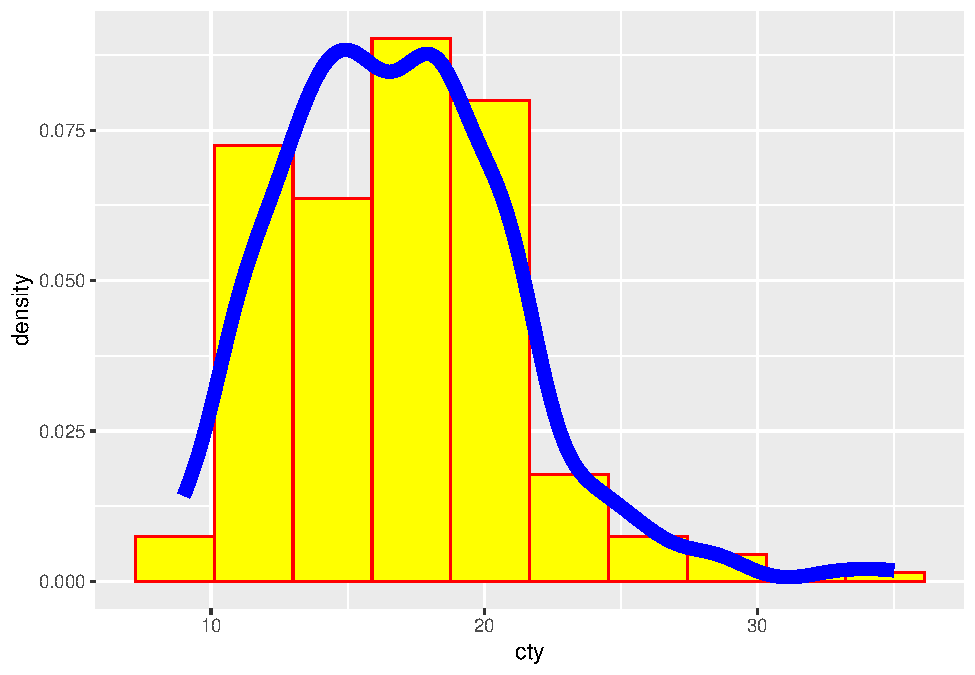
\includegraphics{02_ggplot2_files/figure-latex/unnamed-chunk-5-4.pdf}

\begin{Shaded}
\begin{Highlighting}[]
\CommentTok{\# Adicional (estatístic experimental)}
\FunctionTok{ggplot}\NormalTok{(dados, }\FunctionTok{aes}\NormalTok{(}\AttributeTok{x =}\NormalTok{ drv, }\AttributeTok{y =}\NormalTok{ cty, }\AttributeTok{col =}\NormalTok{ drv)) }\SpecialCharTok{+} 
  \FunctionTok{geom\_boxplot}\NormalTok{()}\SpecialCharTok{+}
  \FunctionTok{theme\_bw}\NormalTok{()}\SpecialCharTok{+}
  \FunctionTok{theme}\NormalTok{(}\AttributeTok{legend.position =} \StringTok{"none"}\NormalTok{)}
\end{Highlighting}
\end{Shaded}

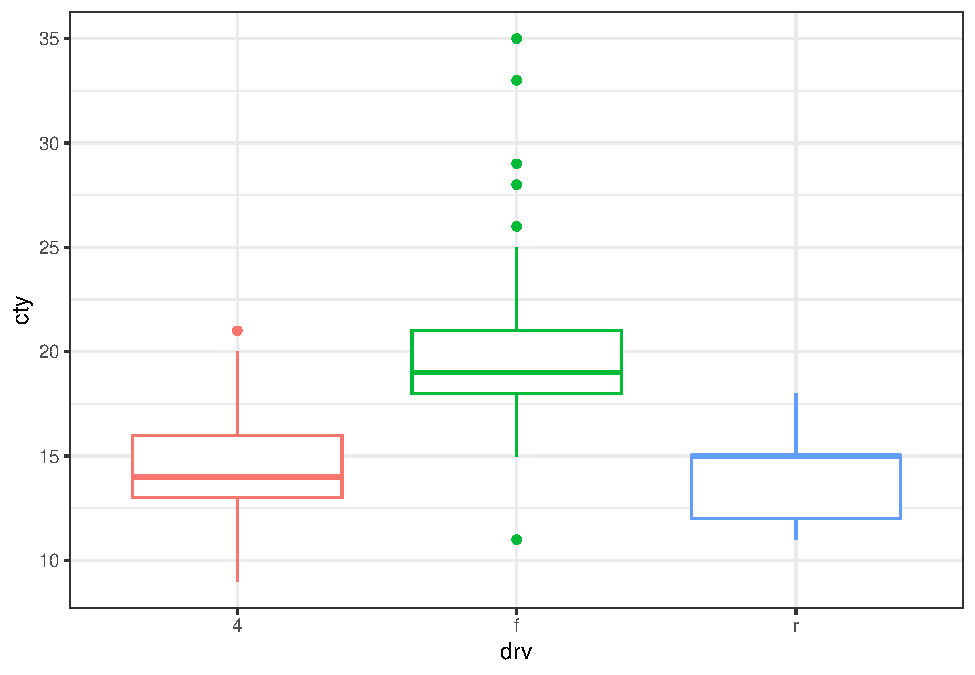
\includegraphics{02_ggplot2_files/figure-latex/unnamed-chunk-5-5.pdf}

\hypertarget{gridextra-e-patchwork}{%
\section{gridExtra e patchwork}\label{gridextra-e-patchwork}}

Alguns links

\href{https://patchwork.data-imaginist.com/articles/guides/assembly.html}{link 1: patchwork}

\href{https://patchwork.data-imaginist.com/articles/patchwork.html}{link 2: patchwork}

\begin{Shaded}
\begin{Highlighting}[]
\CommentTok{\# gridExtra}
\FunctionTok{grid.arrange}\NormalTok{(v1, v2, v3, v4) }
\end{Highlighting}
\end{Shaded}

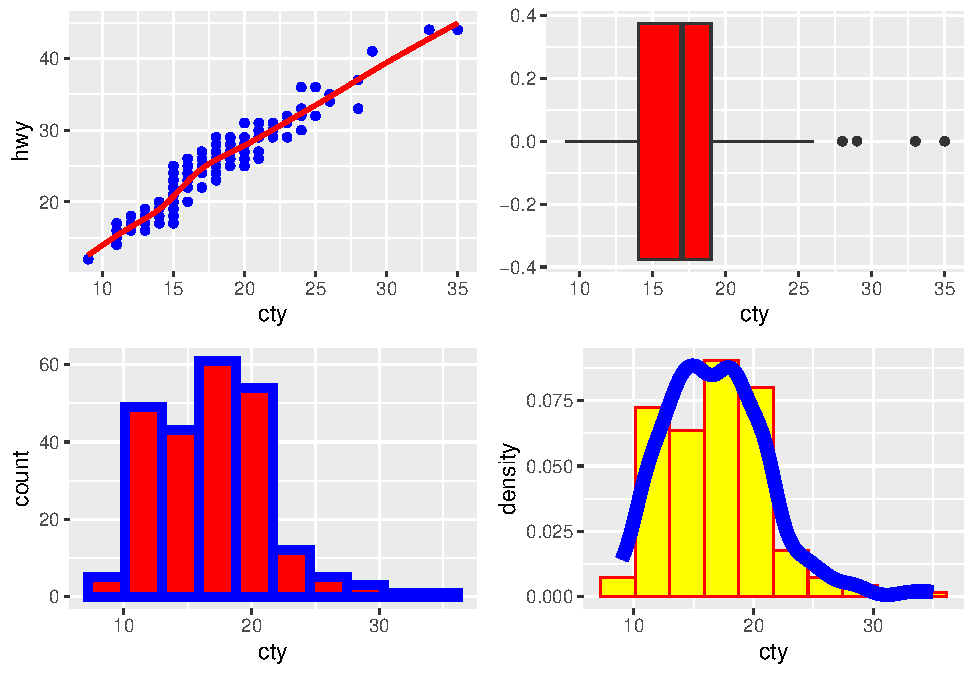
\includegraphics{02_ggplot2_files/figure-latex/unnamed-chunk-6-1.pdf}

\begin{Shaded}
\begin{Highlighting}[]
\CommentTok{\# patchwork}
\NormalTok{v1 }\SpecialCharTok{+}\NormalTok{ v2}
\end{Highlighting}
\end{Shaded}

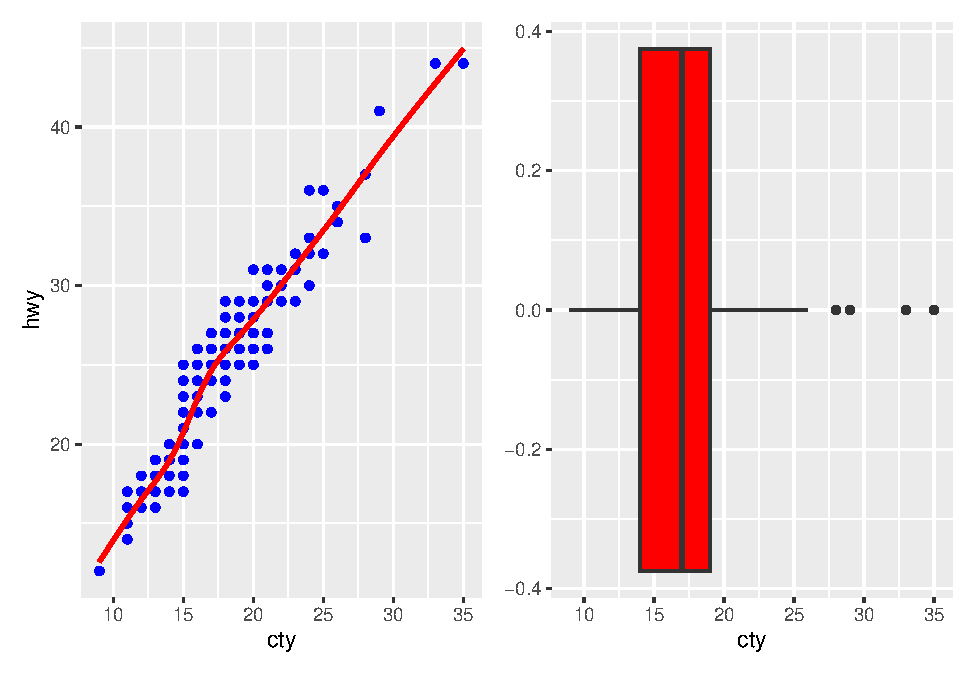
\includegraphics{02_ggplot2_files/figure-latex/unnamed-chunk-6-2.pdf}

\begin{Shaded}
\begin{Highlighting}[]
\NormalTok{v1 }\SpecialCharTok{|}\NormalTok{ v2}
\end{Highlighting}
\end{Shaded}

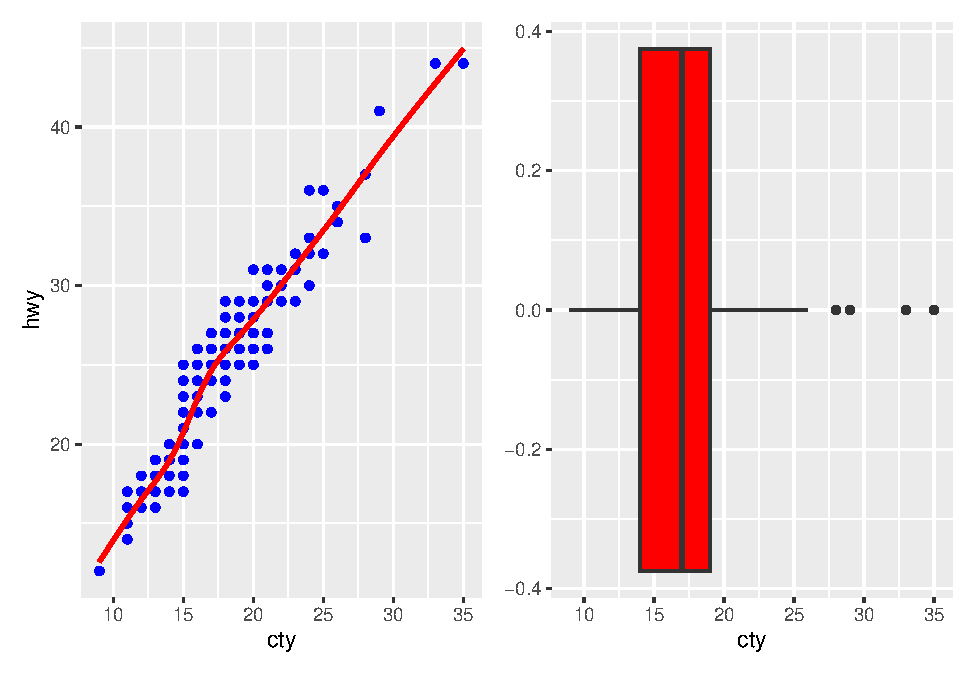
\includegraphics{02_ggplot2_files/figure-latex/unnamed-chunk-6-3.pdf}

\begin{Shaded}
\begin{Highlighting}[]
\NormalTok{v1 }\SpecialCharTok{/}\NormalTok{ v2}
\end{Highlighting}
\end{Shaded}

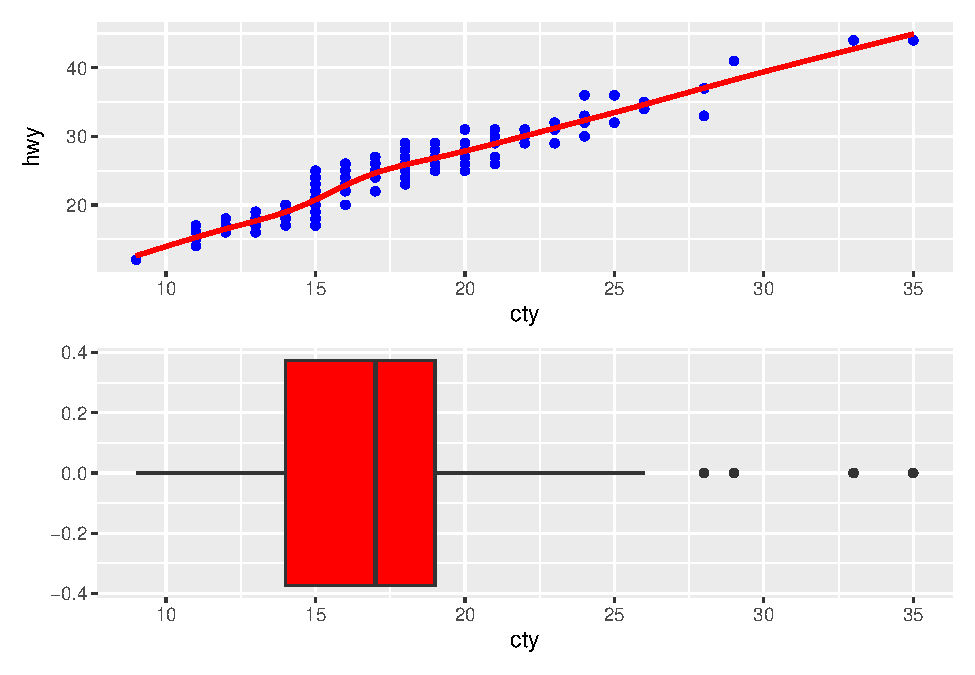
\includegraphics{02_ggplot2_files/figure-latex/unnamed-chunk-6-4.pdf}

\begin{Shaded}
\begin{Highlighting}[]
\NormalTok{v1 }\SpecialCharTok{+}\NormalTok{ v2 }\SpecialCharTok{+}\NormalTok{ v3}
\end{Highlighting}
\end{Shaded}

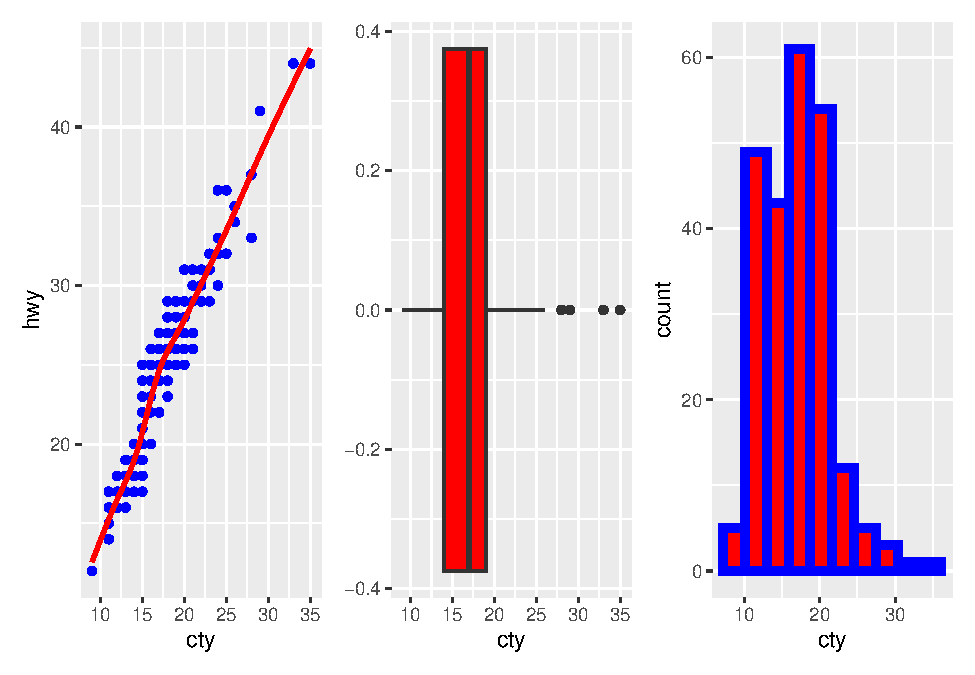
\includegraphics{02_ggplot2_files/figure-latex/unnamed-chunk-6-5.pdf}

\begin{Shaded}
\begin{Highlighting}[]
\NormalTok{v1 }\SpecialCharTok{+}\NormalTok{ (v2 }\SpecialCharTok{+}\NormalTok{ v3)}
\end{Highlighting}
\end{Shaded}

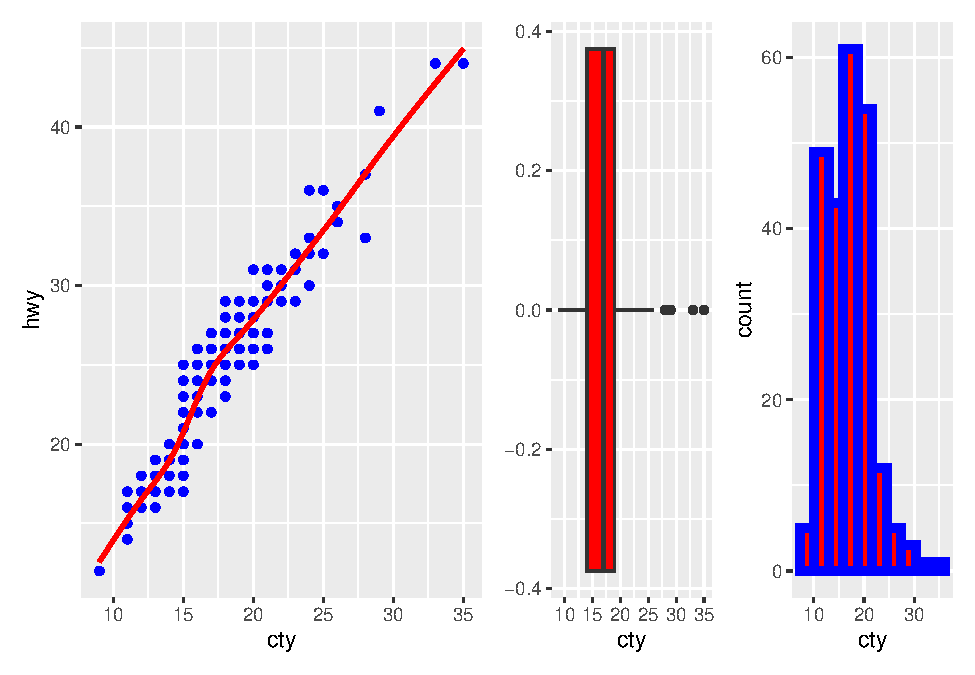
\includegraphics{02_ggplot2_files/figure-latex/unnamed-chunk-6-6.pdf}

\begin{Shaded}
\begin{Highlighting}[]
\NormalTok{v1 }\SpecialCharTok{|}\NormalTok{ (v2 }\SpecialCharTok{/}\NormalTok{ v3)}
\end{Highlighting}
\end{Shaded}

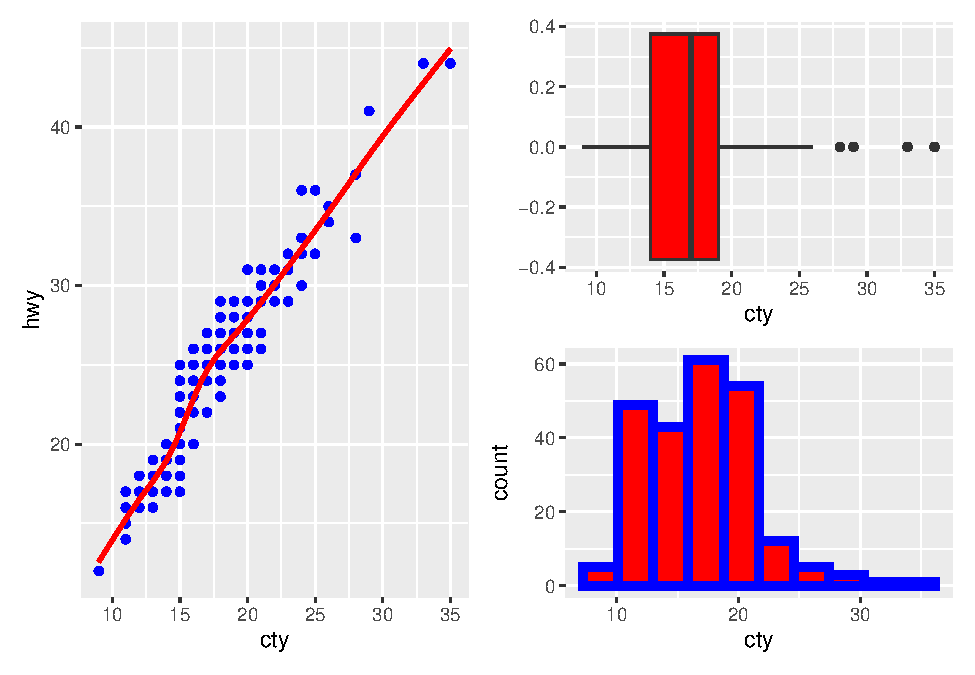
\includegraphics{02_ggplot2_files/figure-latex/unnamed-chunk-6-7.pdf}

\begin{Shaded}
\begin{Highlighting}[]
\NormalTok{v1 }\SpecialCharTok{/}\NormalTok{ (v2 }\SpecialCharTok{+}\NormalTok{ v3)}
\end{Highlighting}
\end{Shaded}

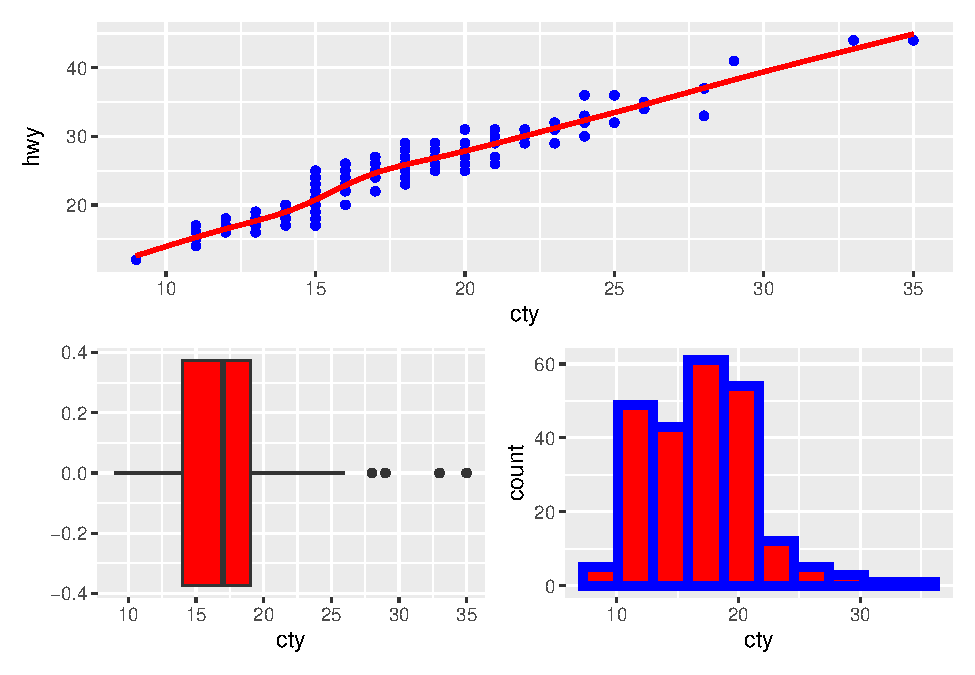
\includegraphics{02_ggplot2_files/figure-latex/unnamed-chunk-6-8.pdf}

\begin{Shaded}
\begin{Highlighting}[]
\NormalTok{v1 }\SpecialCharTok{+}\NormalTok{ v2 }\SpecialCharTok{+}\NormalTok{ v3 }\SpecialCharTok{+}\NormalTok{ v4 }
\end{Highlighting}
\end{Shaded}

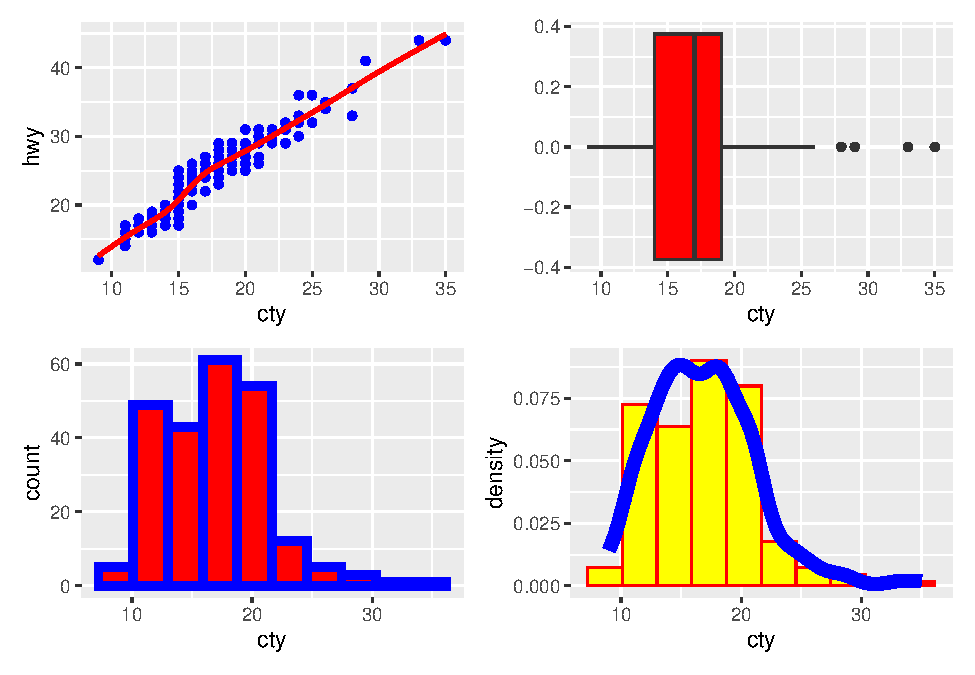
\includegraphics{02_ggplot2_files/figure-latex/unnamed-chunk-6-9.pdf}

\begin{Shaded}
\begin{Highlighting}[]
\NormalTok{v1}\SpecialCharTok{/}\NormalTok{(v2}\SpecialCharTok{+}\NormalTok{v3}\SpecialCharTok{+}\NormalTok{v4)}
\end{Highlighting}
\end{Shaded}

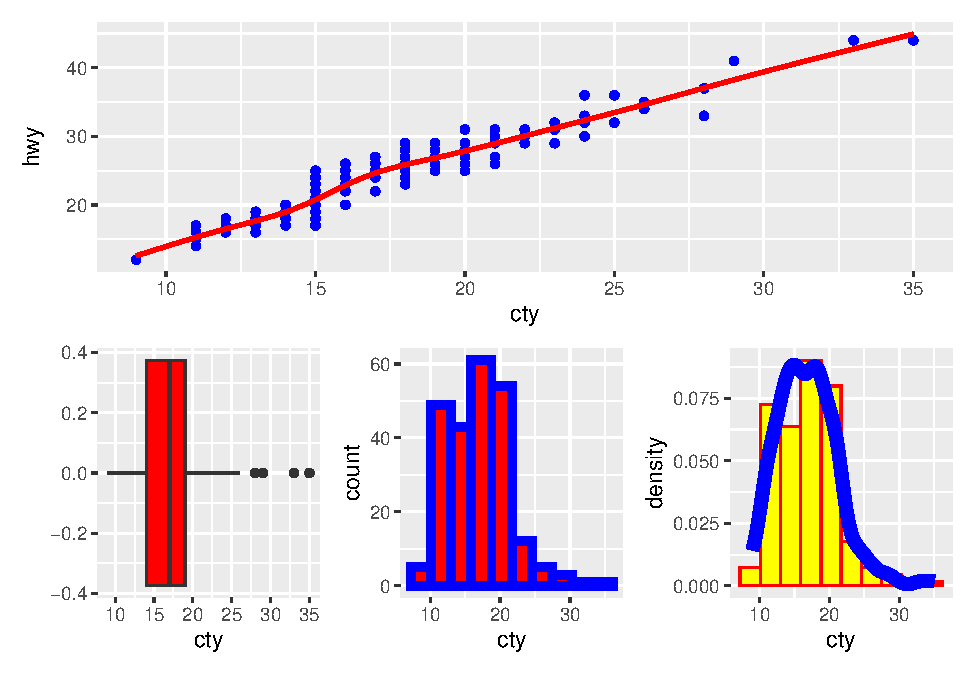
\includegraphics{02_ggplot2_files/figure-latex/unnamed-chunk-6-10.pdf}

\begin{Shaded}
\begin{Highlighting}[]
\NormalTok{v1  }\SpecialCharTok{+}\NormalTok{ (v2 }\SpecialCharTok{+}\NormalTok{ v3 }\SpecialCharTok{+}\NormalTok{ v4)}
\end{Highlighting}
\end{Shaded}

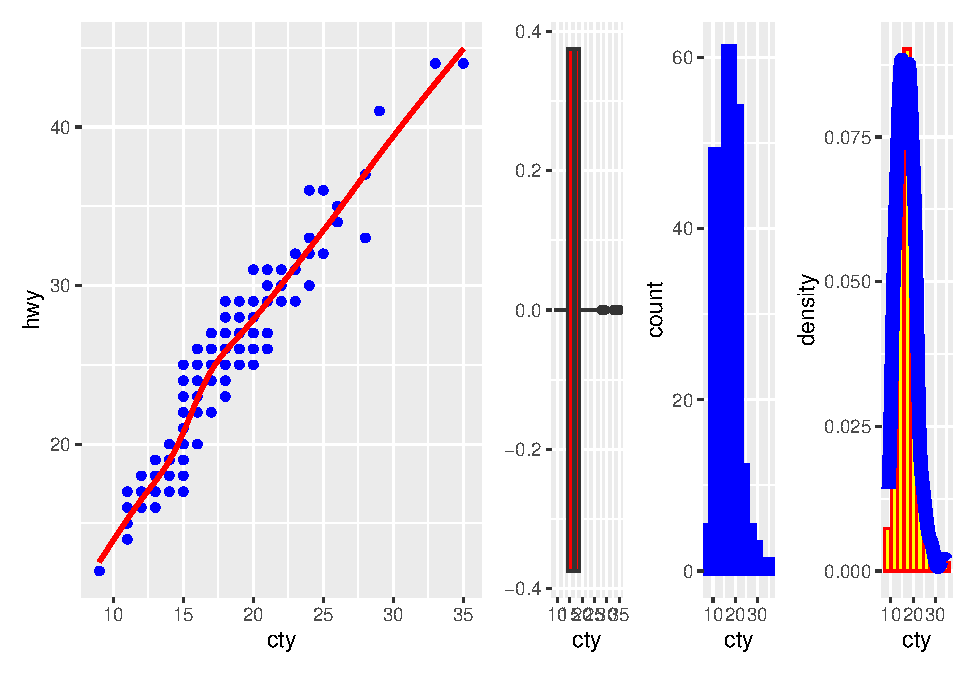
\includegraphics{02_ggplot2_files/figure-latex/unnamed-chunk-6-11.pdf}

\begin{Shaded}
\begin{Highlighting}[]
\NormalTok{v1  }\SpecialCharTok{+}\NormalTok{ v2 }\SpecialCharTok{+}\NormalTok{ (v3 }\SpecialCharTok{+}\NormalTok{ v4)}
\end{Highlighting}
\end{Shaded}

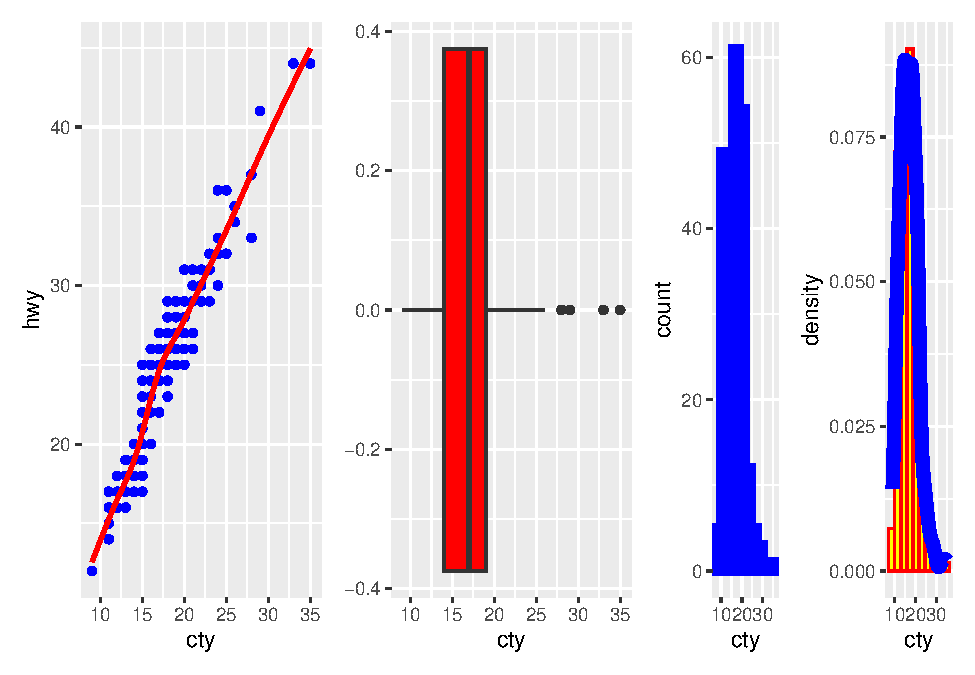
\includegraphics{02_ggplot2_files/figure-latex/unnamed-chunk-6-12.pdf}

\begin{Shaded}
\begin{Highlighting}[]
\NormalTok{(v1 }\SpecialCharTok{|}\NormalTok{ v2 }\SpecialCharTok{|}\NormalTok{ v3) }\SpecialCharTok{/}\NormalTok{ v4}
\end{Highlighting}
\end{Shaded}

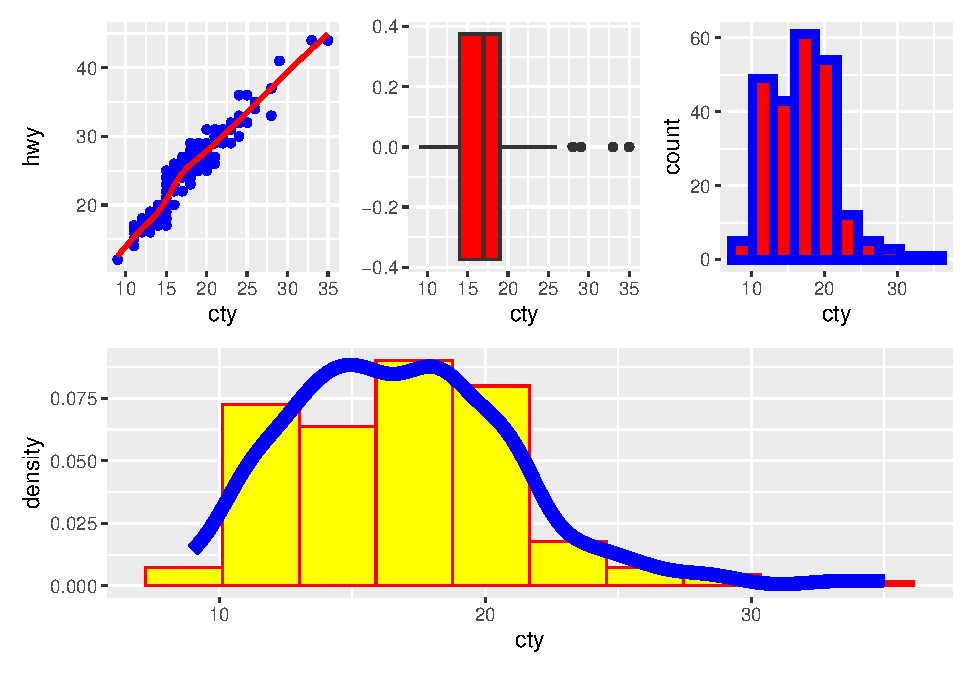
\includegraphics{02_ggplot2_files/figure-latex/unnamed-chunk-6-13.pdf}

\hypertarget{bar-col-density-density2d}{%
\section{bar, col, density, density2d}\label{bar-col-density-density2d}}

\begin{Shaded}
\begin{Highlighting}[]
\NormalTok{v5 }\OtherTok{\textless{}{-}} \FunctionTok{ggplot}\NormalTok{(dados , }\FunctionTok{aes}\NormalTok{(}\AttributeTok{x =}\NormalTok{ manufacturer)) }\SpecialCharTok{+} 
  \FunctionTok{geom\_bar}\NormalTok{()}\SpecialCharTok{+} 
  \FunctionTok{theme}\NormalTok{(}\AttributeTok{axis.text.x =} \FunctionTok{element\_text}\NormalTok{(}\AttributeTok{angle =} \DecValTok{45}\NormalTok{))}
\NormalTok{v5}
\end{Highlighting}
\end{Shaded}

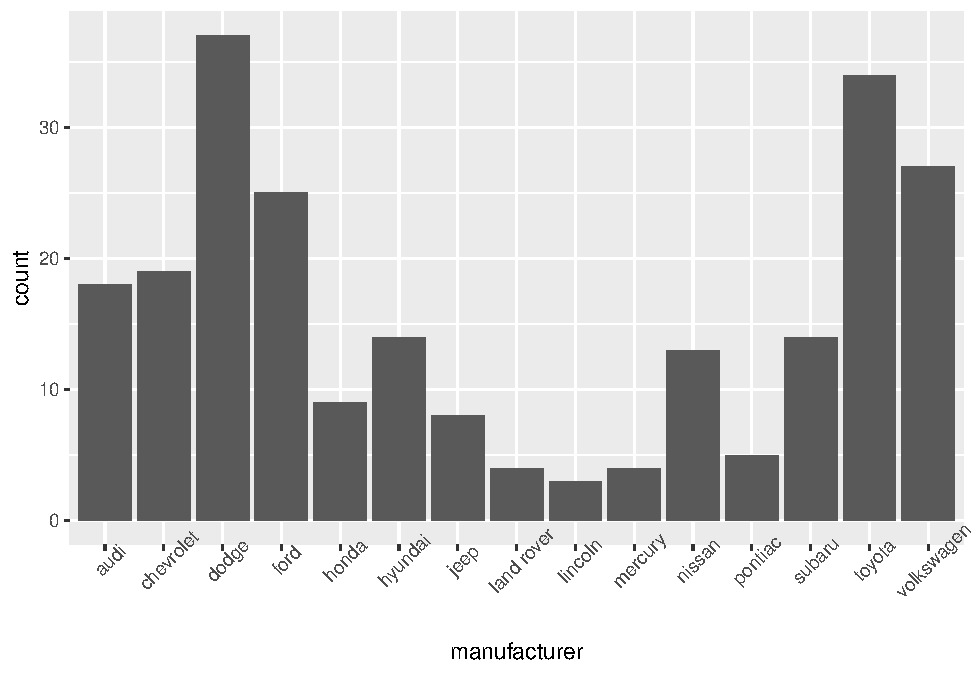
\includegraphics{02_ggplot2_files/figure-latex/unnamed-chunk-7-1.pdf}

\begin{Shaded}
\begin{Highlighting}[]
\CommentTok{\# Dúvidas no geom\_col}
\NormalTok{v6 }\OtherTok{\textless{}{-}} \FunctionTok{ggplot}\NormalTok{(dados , }\FunctionTok{aes}\NormalTok{(}\AttributeTok{x =}\NormalTok{ manufacturer, }\AttributeTok{y =}\NormalTok{ cty)) }\SpecialCharTok{+} 
  \FunctionTok{geom\_col}\NormalTok{()}\SpecialCharTok{+}
  \FunctionTok{theme}\NormalTok{(}\AttributeTok{axis.text.x =} \FunctionTok{element\_text}\NormalTok{(}\AttributeTok{angle =} \DecValTok{45}\NormalTok{))}
\NormalTok{v6}
\end{Highlighting}
\end{Shaded}

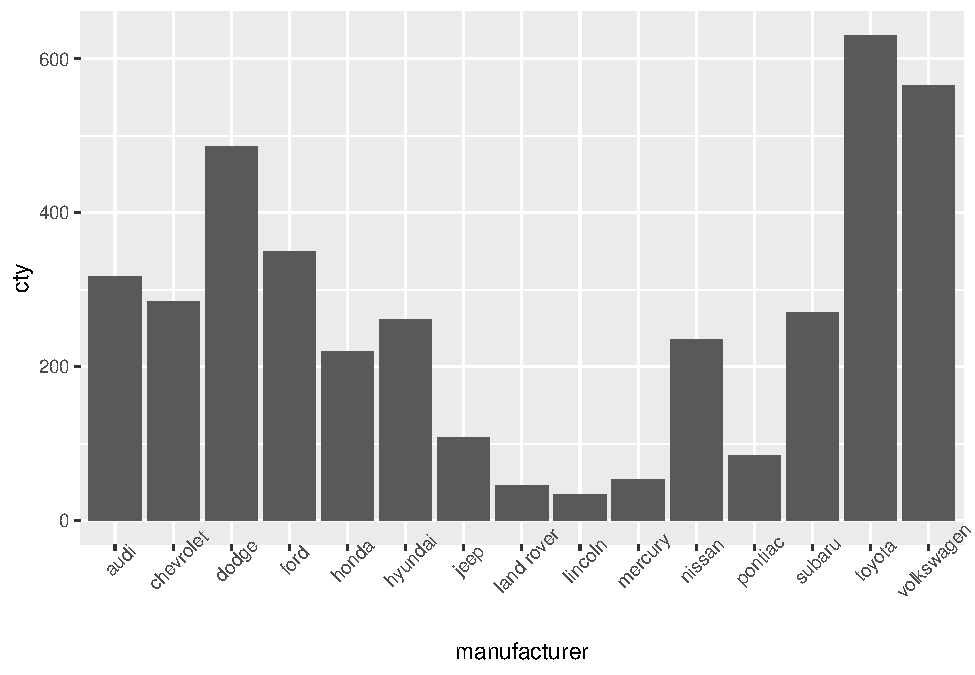
\includegraphics{02_ggplot2_files/figure-latex/unnamed-chunk-7-2.pdf}

\begin{Shaded}
\begin{Highlighting}[]
\NormalTok{dados }\SpecialCharTok{\%\textgreater{}\%} 
  \FunctionTok{select}\NormalTok{(manufacturer, cty) }\SpecialCharTok{\%\textgreater{}\%} 
  \FunctionTok{group\_by}\NormalTok{(manufacturer) }\SpecialCharTok{\%\textgreater{}\%} 
  \FunctionTok{summarise}\NormalTok{(}\AttributeTok{soma\_total\_cty =} \FunctionTok{sum}\NormalTok{(cty),}
            \AttributeTok{n =} \FunctionTok{n}\NormalTok{())}
\end{Highlighting}
\end{Shaded}

\begin{verbatim}
## # A tibble: 15 x 3
##    manufacturer soma_total_cty     n
##    <chr>                 <int> <int>
##  1 audi                    317    18
##  2 chevrolet               285    19
##  3 dodge                   486    37
##  4 ford                    350    25
##  5 honda                   220     9
##  6 hyundai                 261    14
##  7 jeep                    108     8
##  8 land rover               46     4
##  9 lincoln                  34     3
## 10 mercury                  53     4
## 11 nissan                  235    13
## 12 pontiac                  85     5
## 13 subaru                  270    14
## 14 toyota                  630    34
## 15 volkswagen              565    27
\end{verbatim}

\begin{Shaded}
\begin{Highlighting}[]
\CommentTok{\# dados \%\textgreater{}\% }
\CommentTok{\#   filter(manufacturer == "audi") \%\textgreater{}\% }
\CommentTok{\#   select(cty) \%\textgreater{}\% }
\CommentTok{\#   sum()}
\NormalTok{v7 }\OtherTok{\textless{}{-}} \FunctionTok{ggplot}\NormalTok{(dados , }\FunctionTok{aes}\NormalTok{(}\AttributeTok{x =}\NormalTok{ cty)) }\SpecialCharTok{+} 
  \FunctionTok{geom\_density}\NormalTok{()}
\NormalTok{v7}
\end{Highlighting}
\end{Shaded}

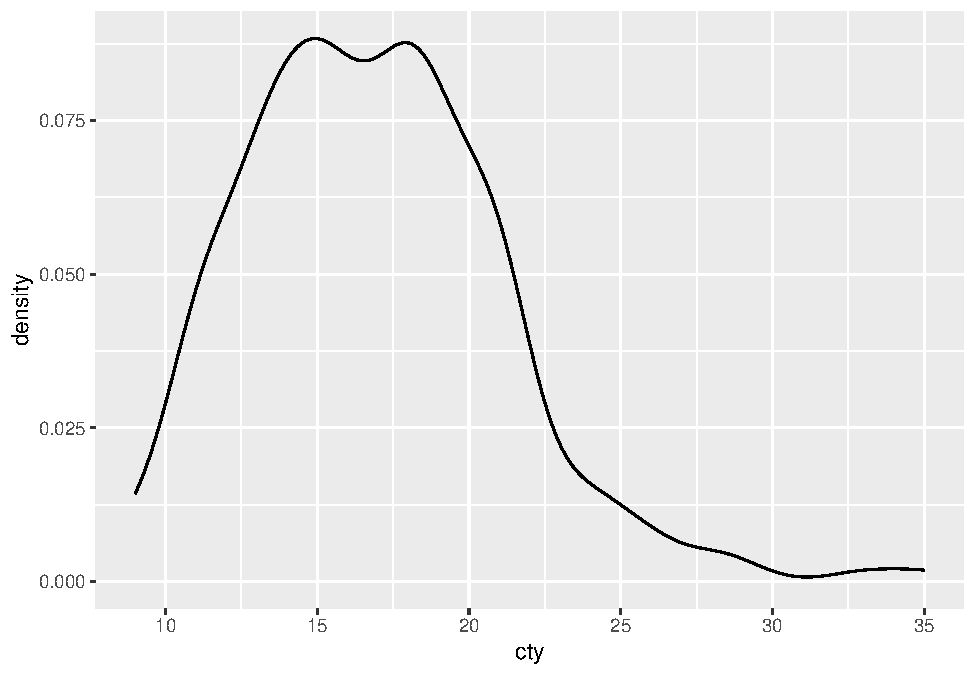
\includegraphics{02_ggplot2_files/figure-latex/unnamed-chunk-7-3.pdf}

\begin{Shaded}
\begin{Highlighting}[]
\NormalTok{v8 }\OtherTok{\textless{}{-}} \FunctionTok{ggplot}\NormalTok{(dados, }\FunctionTok{aes}\NormalTok{(}\AttributeTok{x =}\NormalTok{ cty, }\AttributeTok{y =}\NormalTok{ hwy)) }\SpecialCharTok{+} 
  \FunctionTok{geom\_density2d}\NormalTok{()}\SpecialCharTok{+}
  \FunctionTok{geom\_point}\NormalTok{(}\AttributeTok{colour =} \StringTok{"red"}\NormalTok{)}
\NormalTok{v8}
\end{Highlighting}
\end{Shaded}

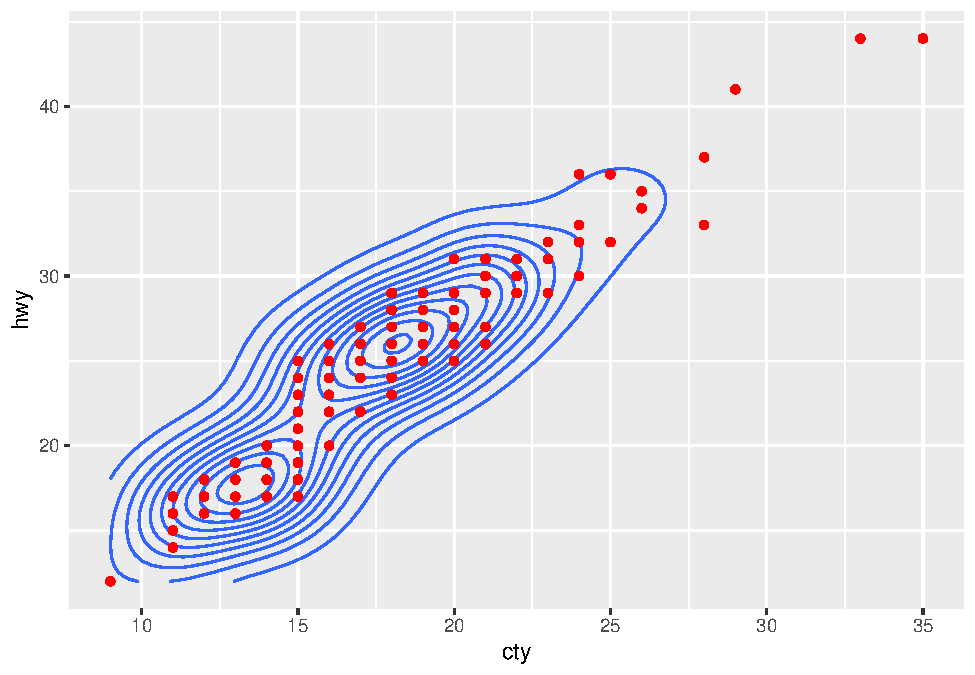
\includegraphics{02_ggplot2_files/figure-latex/unnamed-chunk-7-4.pdf}

\begin{Shaded}
\begin{Highlighting}[]
\NormalTok{(v5}\SpecialCharTok{+}\NormalTok{v6)}\SpecialCharTok{/}\NormalTok{ (v7 }\SpecialCharTok{+}\NormalTok{ v8)}
\end{Highlighting}
\end{Shaded}

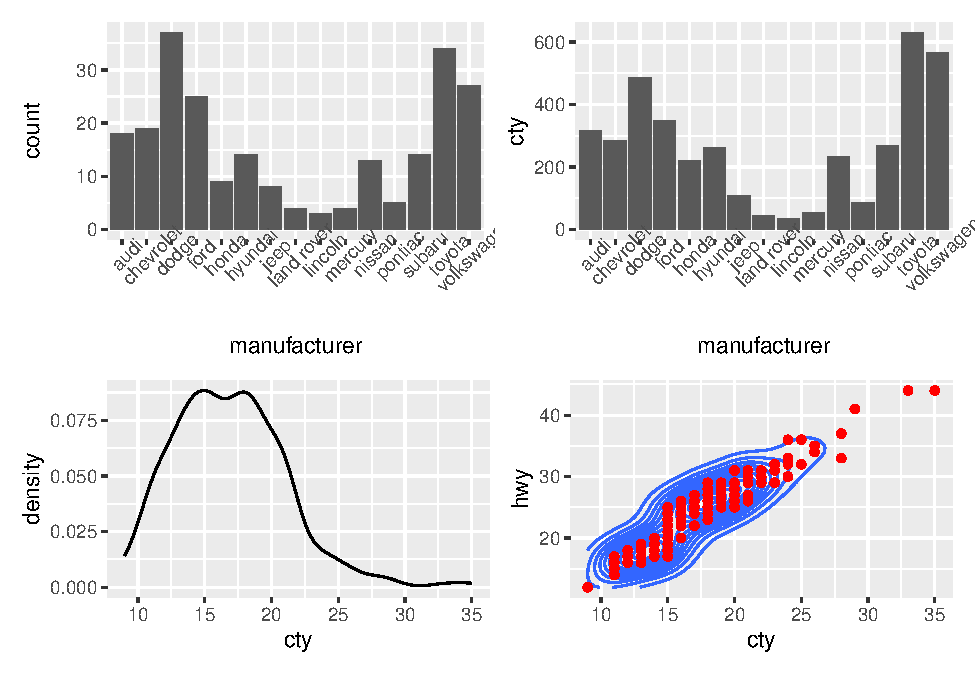
\includegraphics{02_ggplot2_files/figure-latex/unnamed-chunk-7-5.pdf}

\begin{Shaded}
\begin{Highlighting}[]
\CommentTok{\# Deixar pra depois...}
\NormalTok{ dados }\SpecialCharTok{\%\textgreater{}\%} 
    \FunctionTok{select}\NormalTok{(manufacturer, hwy, year) }\SpecialCharTok{\%\textgreater{}\%} 
    \FunctionTok{filter}\NormalTok{(manufacturer }\SpecialCharTok{==} \StringTok{"audi"}\NormalTok{, year }\SpecialCharTok{==} \StringTok{"1999"}\NormalTok{) }\SpecialCharTok{\%\textgreater{}\%} 
    \FunctionTok{summarise}\NormalTok{(}\AttributeTok{media =} \FunctionTok{max}\NormalTok{(hwy))}
\end{Highlighting}
\end{Shaded}

\begin{verbatim}
## # A tibble: 1 x 1
##   media
##   <int>
## 1    29
\end{verbatim}

\begin{Shaded}
\begin{Highlighting}[]
\CommentTok{\# plotly}
\FunctionTok{ggplotly}\NormalTok{(}
\FunctionTok{ggplot}\NormalTok{(dados, }\FunctionTok{aes}\NormalTok{(}\AttributeTok{x =}\NormalTok{ manufacturer, }\AttributeTok{y =}\NormalTok{ hwy, }\AttributeTok{fill =} \FunctionTok{factor}\NormalTok{(year))) }\SpecialCharTok{+} 
  \FunctionTok{geom\_col}\NormalTok{(}\AttributeTok{position =} \StringTok{"dodge"}\NormalTok{) }\SpecialCharTok{+} 
  \FunctionTok{labs}\NormalTok{(}\AttributeTok{fill =} \StringTok{"year"}\NormalTok{) }\SpecialCharTok{+}
  \FunctionTok{theme}\NormalTok{(}\AttributeTok{axis.text.x =} \FunctionTok{element\_text}\NormalTok{(}\AttributeTok{angle =} \DecValTok{45}\NormalTok{)))}

\NormalTok{dados }\SpecialCharTok{\%\textgreater{}\%} \FunctionTok{select}\NormalTok{(manufacturer, hwy, year) }\SpecialCharTok{\%\textgreater{}\%} 
  \FunctionTok{group\_by}\NormalTok{(manufacturer, year) }\SpecialCharTok{\%\textgreater{}\%} 
  \FunctionTok{summarise}\NormalTok{(}\AttributeTok{media =} \FunctionTok{mean}\NormalTok{(hwy))}
\end{Highlighting}
\end{Shaded}

\begin{Shaded}
\begin{Highlighting}[]
\CommentTok{\# Para pensar}

\NormalTok{(dados\_trat }\OtherTok{\textless{}{-}} \FunctionTok{data.frame}\NormalTok{(}\AttributeTok{tratamento =}\NormalTok{ LETTERS[}\DecValTok{1}\SpecialCharTok{:}\DecValTok{3}\NormalTok{], }
                         \AttributeTok{resposta =} \FunctionTok{c}\NormalTok{(}\FloatTok{2.3}\NormalTok{, }\FloatTok{1.9}\NormalTok{, }\FloatTok{3.2}\NormalTok{)))}
\end{Highlighting}
\end{Shaded}

\begin{verbatim}
##   tratamento resposta
## 1          A      2.3
## 2          B      1.9
## 3          C      3.2
\end{verbatim}

\begin{Shaded}
\begin{Highlighting}[]
\FunctionTok{ggplot}\NormalTok{(dados\_trat, }\FunctionTok{aes}\NormalTok{(tratamento, resposta)) }\SpecialCharTok{+}
  \FunctionTok{geom\_col}\NormalTok{(}\AttributeTok{fill =} \StringTok{"red"}\NormalTok{)}
\end{Highlighting}
\end{Shaded}

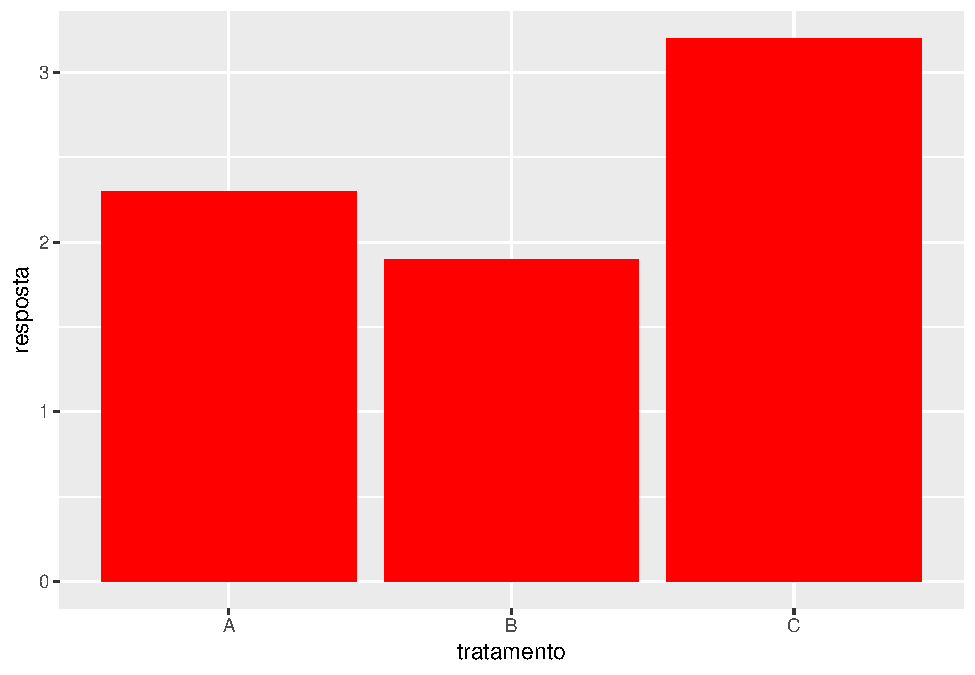
\includegraphics{02_ggplot2_files/figure-latex/unnamed-chunk-9-1.pdf}

\begin{Shaded}
\begin{Highlighting}[]
\CommentTok{\# Mais detalhes...}
\NormalTok{dados }\SpecialCharTok{\%\textgreater{}\%} \FunctionTok{select}\NormalTok{(manufacturer, hwy, year) }\SpecialCharTok{\%\textgreater{}\%} 
  \FunctionTok{group\_by}\NormalTok{(manufacturer, year) }\SpecialCharTok{\%\textgreater{}\%} 
  \FunctionTok{summarise}\NormalTok{(}\AttributeTok{media =} \FunctionTok{mean}\NormalTok{(hwy), }\AttributeTok{.groups =} \StringTok{"drop"}\NormalTok{) }\SpecialCharTok{\%\textgreater{}\%} 
  \FunctionTok{ggplot}\NormalTok{(}\FunctionTok{aes}\NormalTok{(}\AttributeTok{x =}\NormalTok{ manufacturer, }\AttributeTok{y =}\NormalTok{ media, }\AttributeTok{fill =} \FunctionTok{factor}\NormalTok{(year)))}\SpecialCharTok{+}
  \FunctionTok{geom\_col}\NormalTok{(}\AttributeTok{position =} \StringTok{"dodge"}\NormalTok{)}\SpecialCharTok{+}
  \FunctionTok{labs}\NormalTok{(}\AttributeTok{fill =} \StringTok{"year"}\NormalTok{) }\SpecialCharTok{+}
  \FunctionTok{theme}\NormalTok{(}\AttributeTok{axis.text.x =} \FunctionTok{element\_text}\NormalTok{(}\AttributeTok{angle =} \DecValTok{45}\NormalTok{))}
\end{Highlighting}
\end{Shaded}

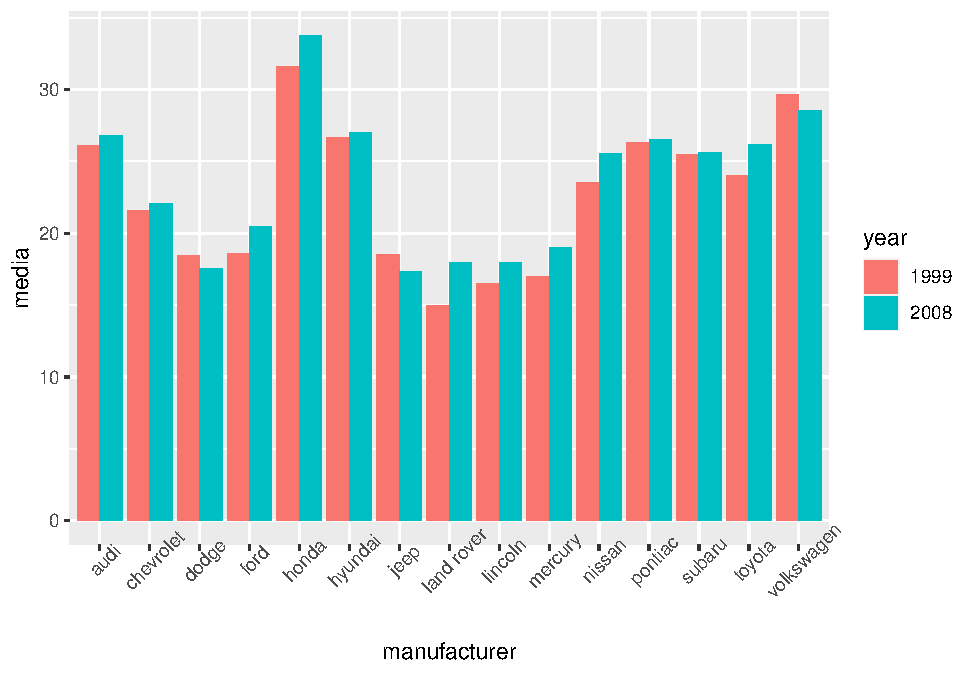
\includegraphics{02_ggplot2_files/figure-latex/unnamed-chunk-9-2.pdf}

\hypertarget{facet_grid-facet_wrap}{%
\section{facet\_grid, facet\_wrap}\label{facet_grid-facet_wrap}}

\begin{Shaded}
\begin{Highlighting}[]
\NormalTok{p1}\OtherTok{\textless{}{-}} \FunctionTok{ggplot}\NormalTok{(dados, }\FunctionTok{aes}\NormalTok{(}\AttributeTok{x =}\NormalTok{ cty, }\AttributeTok{y =}\NormalTok{ hwy)) }\SpecialCharTok{+}
  \FunctionTok{geom\_point}\NormalTok{()}
\NormalTok{p1}
\end{Highlighting}
\end{Shaded}

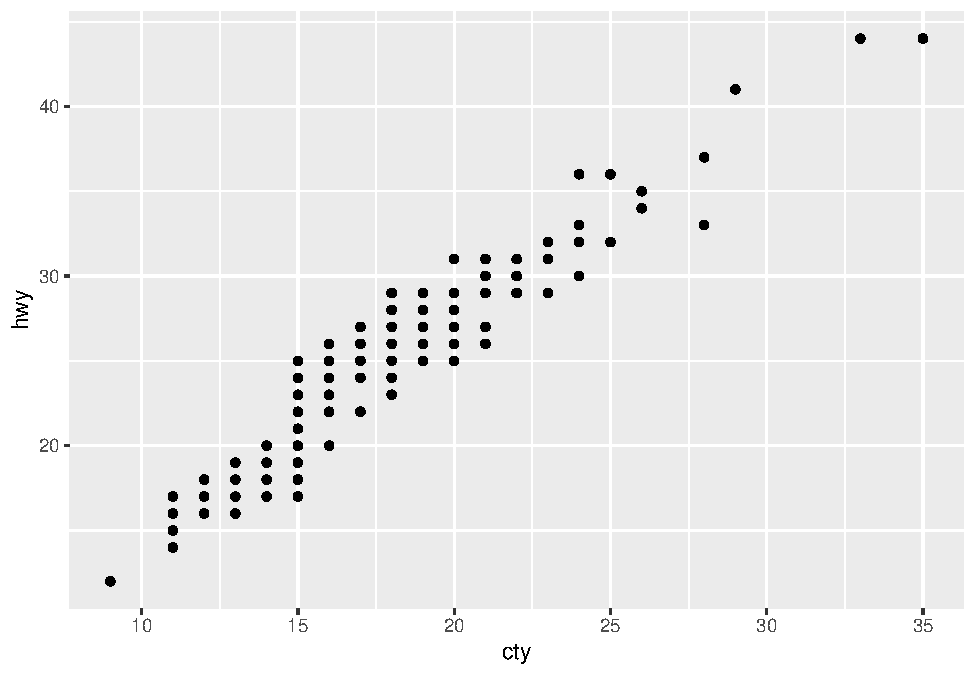
\includegraphics{02_ggplot2_files/figure-latex/unnamed-chunk-10-1.pdf}

\begin{Shaded}
\begin{Highlighting}[]
\NormalTok{p1 }\SpecialCharTok{+} \FunctionTok{facet\_grid}\NormalTok{(}\AttributeTok{rows =} \FunctionTok{vars}\NormalTok{(cyl))}
\end{Highlighting}
\end{Shaded}

\includegraphics{02_ggplot2_files/figure-latex/unnamed-chunk-10-2.pdf}

\begin{Shaded}
\begin{Highlighting}[]
\NormalTok{p1 }\SpecialCharTok{+} \FunctionTok{facet\_grid}\NormalTok{(}\AttributeTok{cols =} \FunctionTok{vars}\NormalTok{(cyl))}
\end{Highlighting}
\end{Shaded}

\includegraphics{02_ggplot2_files/figure-latex/unnamed-chunk-10-3.pdf}

\begin{Shaded}
\begin{Highlighting}[]
\NormalTok{p1 }\SpecialCharTok{+} \FunctionTok{facet\_grid}\NormalTok{(}\SpecialCharTok{\textasciitilde{}}\NormalTok{cyl)}
\end{Highlighting}
\end{Shaded}

\includegraphics{02_ggplot2_files/figure-latex/unnamed-chunk-10-4.pdf}

\begin{Shaded}
\begin{Highlighting}[]
\NormalTok{p1 }\SpecialCharTok{+} \FunctionTok{facet\_grid}\NormalTok{(}\AttributeTok{rows =} \FunctionTok{vars}\NormalTok{(year), }\AttributeTok{cols =}\FunctionTok{vars}\NormalTok{(cyl))}
\end{Highlighting}
\end{Shaded}

\includegraphics{02_ggplot2_files/figure-latex/unnamed-chunk-10-5.pdf}

\begin{Shaded}
\begin{Highlighting}[]
\NormalTok{p1 }\SpecialCharTok{+} \FunctionTok{facet\_grid}\NormalTok{(year}\SpecialCharTok{\textasciitilde{}}\NormalTok{cyl)}
\end{Highlighting}
\end{Shaded}

\includegraphics{02_ggplot2_files/figure-latex/unnamed-chunk-10-6.pdf}

\begin{Shaded}
\begin{Highlighting}[]
\NormalTok{p1 }\SpecialCharTok{+} \FunctionTok{facet\_wrap}\NormalTok{(year }\SpecialCharTok{\textasciitilde{}}\NormalTok{ cyl)}
\end{Highlighting}
\end{Shaded}

\includegraphics{02_ggplot2_files/figure-latex/unnamed-chunk-10-7.pdf}

\begin{Shaded}
\begin{Highlighting}[]
\NormalTok{p1 }\SpecialCharTok{+} \FunctionTok{facet\_wrap}\NormalTok{(cyl }\SpecialCharTok{\textasciitilde{}}\NormalTok{ year)}
\end{Highlighting}
\end{Shaded}

\includegraphics{02_ggplot2_files/figure-latex/unnamed-chunk-10-8.pdf}

\begin{Shaded}
\begin{Highlighting}[]
\NormalTok{p1 }\SpecialCharTok{+} \FunctionTok{facet\_wrap}\NormalTok{(}\SpecialCharTok{\textasciitilde{}}\NormalTok{cyl }\SpecialCharTok{+}\NormalTok{ year)}
\end{Highlighting}
\end{Shaded}

\includegraphics{02_ggplot2_files/figure-latex/unnamed-chunk-10-9.pdf}

\begin{Shaded}
\begin{Highlighting}[]
\NormalTok{p1 }\SpecialCharTok{+} \FunctionTok{facet\_wrap}\NormalTok{(}\SpecialCharTok{\textasciitilde{}}\NormalTok{year }\SpecialCharTok{+}\NormalTok{ cyl)}
\end{Highlighting}
\end{Shaded}

\includegraphics{02_ggplot2_files/figure-latex/unnamed-chunk-10-10.pdf}

\begin{Shaded}
\begin{Highlighting}[]
\NormalTok{p1 }\SpecialCharTok{+} \FunctionTok{facet\_wrap}\NormalTok{(year }\SpecialCharTok{\textasciitilde{}}\NormalTok{ cyl, }\AttributeTok{ncol =} \DecValTok{4}\NormalTok{)}
\end{Highlighting}
\end{Shaded}

\includegraphics{02_ggplot2_files/figure-latex/unnamed-chunk-10-11.pdf}

\begin{Shaded}
\begin{Highlighting}[]
\NormalTok{p1 }\SpecialCharTok{+} \FunctionTok{facet\_wrap}\NormalTok{(cyl }\SpecialCharTok{\textasciitilde{}}\NormalTok{ year, }\AttributeTok{ncol =} \DecValTok{4}\NormalTok{)}
\end{Highlighting}
\end{Shaded}

\includegraphics{02_ggplot2_files/figure-latex/unnamed-chunk-10-12.pdf}

\hypertarget{stat_function}{%
\section{stat\_function}\label{stat_function}}

\begin{Shaded}
\begin{Highlighting}[]
\NormalTok{a}\OtherTok{\textless{}{-}} \SpecialCharTok{{-}}\DecValTok{3} \CommentTok{\# média}
\NormalTok{b}\OtherTok{\textless{}{-}} \DecValTok{4}  \CommentTok{\# desv. padrão}
\FunctionTok{ggplot}\NormalTok{(}\FunctionTok{data.frame}\NormalTok{(}\AttributeTok{x =} \FunctionTok{c}\NormalTok{(a }\SpecialCharTok{{-}} \DecValTok{3}\SpecialCharTok{*}\NormalTok{b, a }\SpecialCharTok{+} \DecValTok{3}\SpecialCharTok{*}\NormalTok{b)), }\FunctionTok{aes}\NormalTok{(x)) }\SpecialCharTok{+} 
  \FunctionTok{stat\_function}\NormalTok{(}\AttributeTok{fun =}\NormalTok{ dnorm, }\AttributeTok{args =} \FunctionTok{list}\NormalTok{(}\AttributeTok{mean =}\NormalTok{ a, }\AttributeTok{sd =}\NormalTok{ b))}\SpecialCharTok{+}
  \FunctionTok{geom\_vline}\NormalTok{(}\AttributeTok{xintercept =} \FunctionTok{c}\NormalTok{(a }\SpecialCharTok{{-}} \DecValTok{3}\SpecialCharTok{*}\NormalTok{b, a, a }\SpecialCharTok{+} \DecValTok{3}\SpecialCharTok{*}\NormalTok{b), }\AttributeTok{col =} \StringTok{"red"}\NormalTok{, }\AttributeTok{lty =} \DecValTok{2}\NormalTok{)}\SpecialCharTok{+}
  \FunctionTok{theme\_minimal}\NormalTok{()}
\end{Highlighting}
\end{Shaded}

\includegraphics{02_ggplot2_files/figure-latex/unnamed-chunk-11-1.pdf}

\hypertarget{stat_summary}{%
\section{stat\_summary}\label{stat_summary}}

\begin{Shaded}
\begin{Highlighting}[]
\FunctionTok{ggplot}\NormalTok{(dados, }\FunctionTok{aes}\NormalTok{(}\AttributeTok{x =}\NormalTok{ manufacturer, }\AttributeTok{y =}\NormalTok{ hwy)) }\SpecialCharTok{+} 
  \FunctionTok{geom\_boxplot}\NormalTok{()}\SpecialCharTok{+}
  \FunctionTok{geom\_point}\NormalTok{(}\AttributeTok{col =} \StringTok{"red"}\NormalTok{, }\AttributeTok{size=}\FloatTok{0.8}\NormalTok{)}\SpecialCharTok{+}
  \FunctionTok{stat\_summary}\NormalTok{(}\AttributeTok{fun =}\NormalTok{ mean, }\AttributeTok{col =} \StringTok{"blue"}\NormalTok{)}\SpecialCharTok{+}
  \FunctionTok{theme\_minimal}\NormalTok{()}\SpecialCharTok{+}
  \FunctionTok{theme}\NormalTok{(}\AttributeTok{axis.text.x =} \FunctionTok{element\_text}\NormalTok{(}\AttributeTok{angle =} \DecValTok{45}\NormalTok{))}
\end{Highlighting}
\end{Shaded}

\includegraphics{02_ggplot2_files/figure-latex/unnamed-chunk-12-1.pdf}

\hypertarget{theme_}{%
\section{theme\_*()}\label{theme_}}

\begin{Shaded}
\begin{Highlighting}[]
\NormalTok{a1}\OtherTok{\textless{}{-}}\NormalTok{ p1 }\SpecialCharTok{+} \FunctionTok{theme\_bw}\NormalTok{() }\SpecialCharTok{+} \FunctionTok{labs}\NormalTok{(}\AttributeTok{title =} \StringTok{"theme\_bw()"}\NormalTok{)}
\NormalTok{a2}\OtherTok{\textless{}{-}}\NormalTok{ p1 }\SpecialCharTok{+} \FunctionTok{theme\_classic}\NormalTok{() }\SpecialCharTok{+} \FunctionTok{labs}\NormalTok{(}\AttributeTok{title =} \StringTok{"theme\_classic()"}\NormalTok{)}
\NormalTok{a3}\OtherTok{\textless{}{-}}\NormalTok{ p1 }\SpecialCharTok{+} \FunctionTok{theme\_light}\NormalTok{() }\SpecialCharTok{+} \FunctionTok{labs}\NormalTok{(}\AttributeTok{title =} \StringTok{"theme\_light()"}\NormalTok{)}
\NormalTok{a4}\OtherTok{\textless{}{-}}\NormalTok{ p1 }\SpecialCharTok{+} \FunctionTok{theme\_minimal}\NormalTok{() }\SpecialCharTok{+} \FunctionTok{labs}\NormalTok{(}\AttributeTok{title =} \StringTok{"theme\_minimal()"}\NormalTok{)}

\NormalTok{a1 }\SpecialCharTok{+}\NormalTok{ a2 }\SpecialCharTok{+}\NormalTok{ a3 }\SpecialCharTok{+}\NormalTok{ a4}
\end{Highlighting}
\end{Shaded}

\includegraphics{02_ggplot2_files/figure-latex/unnamed-chunk-13-1.pdf}

\hypertarget{gruxe1fico-de-perfis-spaguetti-plot}{%
\section{Gráfico de perfis (Spaguetti plot)}\label{gruxe1fico-de-perfis-spaguetti-plot}}

\begin{Shaded}
\begin{Highlighting}[]
\FunctionTok{glimpse}\NormalTok{(Orange)}
\end{Highlighting}
\end{Shaded}

\begin{verbatim}
## Rows: 35
## Columns: 3
## $ Tree          <ord> 1, 1, 1, 1, 1, 1, 1, 2, 2, 2, 2, 2, 2, 2, 3, 3, 3, 3, 3,~
## $ age           <dbl> 118, 484, 664, 1004, 1231, 1372, 1582, 118, 484, 664, 10~
## $ circumference <dbl> 30, 58, 87, 115, 120, 142, 145, 33, 69, 111, 156, 172, 2~
\end{verbatim}

\begin{Shaded}
\begin{Highlighting}[]
\FunctionTok{ggplot}\NormalTok{(Orange, }\FunctionTok{aes}\NormalTok{(}\AttributeTok{x =}\NormalTok{ age, }\AttributeTok{y =}\NormalTok{ circumference, }\AttributeTok{group =}\NormalTok{ Tree, }
                   \AttributeTok{col =}\NormalTok{ Tree)) }\SpecialCharTok{+}
  \FunctionTok{geom\_line}\NormalTok{()}\SpecialCharTok{+}
  \FunctionTok{stat\_summary}\NormalTok{(}\FunctionTok{aes}\NormalTok{(}\AttributeTok{group =} \DecValTok{1}\NormalTok{), }\AttributeTok{fun =}\NormalTok{ mean, }\AttributeTok{col =} \StringTok{"red"}\NormalTok{, }
               \AttributeTok{geom =} \StringTok{"line"}\NormalTok{, }\AttributeTok{size =} \DecValTok{1}\NormalTok{, }\AttributeTok{show.legend =} \ConstantTok{FALSE}\NormalTok{,}
               \AttributeTok{linetype =} \DecValTok{2}\NormalTok{)}\SpecialCharTok{+}
  \FunctionTok{xlim}\NormalTok{(}\DecValTok{0}\NormalTok{, }\DecValTok{1600}\NormalTok{)}\SpecialCharTok{+}
  \FunctionTok{theme\_minimal}\NormalTok{()}
\end{Highlighting}
\end{Shaded}

\includegraphics{02_ggplot2_files/figure-latex/unnamed-chunk-14-1.pdf}

\begin{Shaded}
\begin{Highlighting}[]
\FunctionTok{ggplot}\NormalTok{(Orange, }\FunctionTok{aes}\NormalTok{(}\AttributeTok{x =}\NormalTok{ age, }\AttributeTok{y =}\NormalTok{ circumference, }\AttributeTok{group =}\NormalTok{ Tree)) }\SpecialCharTok{+}
  \FunctionTok{geom\_line}\NormalTok{()}\SpecialCharTok{+}
  \FunctionTok{xlim}\NormalTok{(}\DecValTok{0}\NormalTok{, }\DecValTok{1600}\NormalTok{)}\SpecialCharTok{+}
  \FunctionTok{facet\_wrap}\NormalTok{(}\SpecialCharTok{\textasciitilde{}}\NormalTok{Tree)}\SpecialCharTok{+}
  \FunctionTok{theme\_minimal}\NormalTok{()}\SpecialCharTok{+}
  \FunctionTok{theme}\NormalTok{(}\AttributeTok{legend.position =} \StringTok{"none"}\NormalTok{)}
\end{Highlighting}
\end{Shaded}

\includegraphics{02_ggplot2_files/figure-latex/unnamed-chunk-14-2.pdf}

\hypertarget{plotly}{%
\section{plotly}\label{plotly}}

\href{https://cran.r-project.org/web/packages/plotly/index.html}{plotly cran}

\href{https://plotly-r.com/}{Interactive web-based data visualization with R, plotly, and shiny}

\href{https://plotly.com/r/}{Plotly R Open Source Graphing Library}

\begin{Shaded}
\begin{Highlighting}[]
\FunctionTok{ggplotly}\NormalTok{(v1)}
\FunctionTok{ggplotly}\NormalTok{(v2)}
\FunctionTok{ggplotly}\NormalTok{(v4)}
\FunctionTok{ggplotly}\NormalTok{(v5)}
\end{Highlighting}
\end{Shaded}

\hypertarget{esquisse}{%
\section{esquisse}\label{esquisse}}

Alguns links de interesse

\href{https://cran.r-project.org/web/packages/esquisse/vignettes/get-started.html}{esquisse}

\href{https://cran.r-project.org/web/packages/esquisse/vignettes/shiny-usage.html}{esquisse + shiny}

\begin{Shaded}
\begin{Highlighting}[]
\FunctionTok{esquisser}\NormalTok{(dados)}
\end{Highlighting}
\end{Shaded}

\hypertarget{exemplo-esquisse}{%
\section{Exemplo esquisse}\label{exemplo-esquisse}}

\begin{Shaded}
\begin{Highlighting}[]
\FunctionTok{ggplot}\NormalTok{(dados) }\SpecialCharTok{+}
  \FunctionTok{aes}\NormalTok{(}\AttributeTok{x =}\NormalTok{ displ, }\AttributeTok{y =}\NormalTok{ hwy, }\AttributeTok{colour =}\NormalTok{ drv) }\SpecialCharTok{+}
  \FunctionTok{geom\_point}\NormalTok{(}\AttributeTok{shape =} \StringTok{"circle"}\NormalTok{, }\AttributeTok{size =} \FloatTok{1.85}\NormalTok{) }\SpecialCharTok{+}
  \FunctionTok{scale\_color\_hue}\NormalTok{(}\AttributeTok{direction =} \DecValTok{1}\NormalTok{) }\SpecialCharTok{+}
  \FunctionTok{theme\_minimal}\NormalTok{() }\SpecialCharTok{+}
  \FunctionTok{theme}\NormalTok{(}\AttributeTok{legend.position =} \StringTok{"top"}\NormalTok{)}
\end{Highlighting}
\end{Shaded}

\includegraphics{02_ggplot2_files/figure-latex/unnamed-chunk-17-1.pdf}

\begin{Shaded}
\begin{Highlighting}[]
\FunctionTok{ggplot}\NormalTok{(dados) }\SpecialCharTok{+}
  \FunctionTok{aes}\NormalTok{(}\AttributeTok{x =}\NormalTok{ displ, }\AttributeTok{y =}\NormalTok{ cty, }\AttributeTok{colour =}\NormalTok{ class, }\AttributeTok{size =}\NormalTok{ cty) }\SpecialCharTok{+}
  \FunctionTok{geom\_point}\NormalTok{(}\AttributeTok{shape =} \StringTok{"circle"}\NormalTok{) }\SpecialCharTok{+}
  \FunctionTok{scale\_color\_hue}\NormalTok{(}\AttributeTok{direction =} \DecValTok{1}\NormalTok{) }\SpecialCharTok{+}
  \FunctionTok{theme}\NormalTok{(}\AttributeTok{legend.position =} \StringTok{"top"}\NormalTok{) }\SpecialCharTok{+}
  \FunctionTok{facet\_wrap}\NormalTok{(}\FunctionTok{vars}\NormalTok{(drv))}
\end{Highlighting}
\end{Shaded}

\includegraphics{02_ggplot2_files/figure-latex/unnamed-chunk-18-1.pdf}

\hypertarget{purrr}{%
\chapter{purrr}\label{purrr}}

\begin{Shaded}
\begin{Highlighting}[]
\FunctionTok{library}\NormalTok{(tidyverse)}
\FunctionTok{ls}\NormalTok{(}\StringTok{"package:purrr"}\NormalTok{)}
\end{Highlighting}
\end{Shaded}

\begin{verbatim}
##   [1] "%@%"                 "%||%"                "%>%"                
##   [4] "accumulate"          "accumulate_right"    "accumulate2"        
##   [7] "array_branch"        "array_tree"          "as_mapper"          
##  [10] "as_vector"           "assign_in"           "at_depth"           
##  [13] "attr_getter"         "auto_browse"         "chuck"              
##  [16] "compact"             "compose"             "cross"              
##  [19] "cross_d"             "cross_df"            "cross_n"            
##  [22] "cross2"              "cross3"              "detect"             
##  [25] "detect_index"        "discard"             "discard_at"         
##  [28] "done"                "every"               "exec"               
##  [31] "flatten"             "flatten_chr"         "flatten_dbl"        
##  [34] "flatten_df"          "flatten_dfc"         "flatten_dfr"        
##  [37] "flatten_int"         "flatten_lgl"         "flatten_raw"        
##  [40] "has_element"         "head_while"          "imap"               
##  [43] "imap_chr"            "imap_dbl"            "imap_dfc"           
##  [46] "imap_dfr"            "imap_int"            "imap_lgl"           
##  [49] "imap_raw"            "imodify"             "insistently"        
##  [52] "invoke"              "invoke_map"          "invoke_map_chr"     
##  [55] "invoke_map_dbl"      "invoke_map_df"       "invoke_map_dfc"     
##  [58] "invoke_map_dfr"      "invoke_map_int"      "invoke_map_lgl"     
##  [61] "invoke_map_raw"      "is_atomic"           "is_bare_atomic"     
##  [64] "is_bare_character"   "is_bare_double"      "is_bare_integer"    
##  [67] "is_bare_list"        "is_bare_logical"     "is_bare_numeric"    
##  [70] "is_bare_vector"      "is_character"        "is_double"          
##  [73] "is_empty"            "is_formula"          "is_function"        
##  [76] "is_integer"          "is_list"             "is_logical"         
##  [79] "is_null"             "is_rate"             "is_scalar_atomic"   
##  [82] "is_scalar_character" "is_scalar_double"    "is_scalar_integer"  
##  [85] "is_scalar_list"      "is_scalar_logical"   "is_scalar_vector"   
##  [88] "is_vector"           "iwalk"               "keep"               
##  [91] "keep_at"             "lift"                "lift_dl"            
##  [94] "lift_dv"             "lift_ld"             "lift_lv"            
##  [97] "lift_vd"             "lift_vl"             "list_along"         
## [100] "list_assign"         "list_c"              "list_cbind"         
## [103] "list_flatten"        "list_merge"          "list_modify"        
## [106] "list_rbind"          "list_simplify"       "list_transpose"     
## [109] "lmap"                "lmap_at"             "lmap_if"            
## [112] "map"                 "map_at"              "map_chr"            
## [115] "map_dbl"             "map_depth"           "map_df"             
## [118] "map_dfc"             "map_dfr"             "map_if"             
## [121] "map_int"             "map_lgl"             "map_raw"            
## [124] "map_vec"             "map2"                "map2_chr"           
## [127] "map2_dbl"            "map2_df"             "map2_dfc"           
## [130] "map2_dfr"            "map2_int"            "map2_lgl"           
## [133] "map2_raw"            "map2_vec"            "modify"             
## [136] "modify_at"           "modify_depth"        "modify_if"          
## [139] "modify_in"           "modify_tree"         "modify2"            
## [142] "negate"              "none"                "partial"            
## [145] "pluck"               "pluck_depth"         "pluck_exists"       
## [148] "pluck<-"             "pmap"                "pmap_chr"           
## [151] "pmap_dbl"            "pmap_df"             "pmap_dfc"           
## [154] "pmap_dfr"            "pmap_int"            "pmap_lgl"           
## [157] "pmap_raw"            "pmap_vec"            "possibly"           
## [160] "prepend"             "pwalk"               "quietly"            
## [163] "rate_backoff"        "rate_delay"          "rate_reset"         
## [166] "rate_sleep"          "rbernoulli"          "rdunif"             
## [169] "reduce"              "reduce_right"        "reduce2"            
## [172] "reduce2_right"       "rep_along"           "rerun"              
## [175] "safely"              "set_names"           "simplify"           
## [178] "simplify_all"        "slowly"              "some"               
## [181] "splice"              "tail_while"          "transpose"          
## [184] "update_list"         "vec_depth"           "walk"               
## [187] "walk2"               "when"                "zap"
\end{verbatim}

\hypertarget{map-functions}{%
\section{map functions}\label{map-functions}}

\begin{Shaded}
\begin{Highlighting}[]
\FunctionTok{example}\NormalTok{(}\StringTok{"map"}\NormalTok{)}
\end{Highlighting}
\end{Shaded}

\begin{verbatim}
## 
## map> # Compute normal distributions from an atomic vector
## map> 1:10 |>
## map+   map(rnorm, n = 10)
## [[1]]
##  [1] 1.2552665 2.0536152 0.7115246 1.5852292 1.1822990 2.3229330 1.2888130
##  [8] 0.8643425 1.8043964 1.6049015
## 
## [[2]]
##  [1] 2.76722104 1.38470163 0.07290803 4.11042691 0.66904733 2.26320055
##  [7] 3.10270087 1.24885123 3.70539375 3.01792371
## 
## [[3]]
##  [1] 1.401737 2.799868 3.494463 1.883361 3.967113 3.072678 4.526046 3.149554
##  [9] 2.562065 2.547237
## 
## [[4]]
##  [1] 4.355527 3.604107 4.043125 3.789485 4.965378 4.154317 3.844999 4.309209
##  [9] 3.925635 3.256635
## 
## [[5]]
##  [1] 5.169386 7.072597 5.090708 5.314264 5.796984 3.774043 4.315370 5.363939
##  [9] 2.990695 5.746886
## 
## [[6]]
##  [1] 7.822415 6.417261 4.479506 6.533698 6.391653 6.916601 5.068146 7.813064
##  [9] 5.473113 5.572169
## 
## [[7]]
##  [1] 7.237784 5.614913 7.122572 7.501402 5.848908 7.199973 7.583485 4.981665
##  [9] 6.317422 8.311529
## 
## [[8]]
##  [1] 8.202467 7.223986 7.316062 6.855017 9.184348 8.389047 7.574641 7.665256
##  [9] 6.581578 7.786203
## 
## [[9]]
##  [1] 9.269320 7.568131 7.399557 8.696145 9.514198 8.912879 9.546866 8.740105
##  [9] 9.075741 9.658302
## 
## [[10]]
##  [1] 10.783664  9.934881  9.301359  9.280198  9.246359 10.471550  8.970142
##  [8] 10.435153  8.953879  9.442058
## 
## 
## map> # You can also use an anonymous function
## map> 1:10 |>
## map+   map(\(x) rnorm(10, x))
## [[1]]
##  [1]  2.12388734  0.30857603  1.57903557  1.72158284 -0.07462741  1.07887850
##  [7]  0.33498143  0.02750241  1.67329193  3.15962570
## 
## [[2]]
##  [1] 0.3622147 1.0157929 2.3557127 2.9839268 2.3761189 0.4922985 2.2394546
##  [8] 3.3963837 2.3739279 3.4977326
## 
## [[3]]
##  [1] 3.421281 3.671517 2.483015 3.214577 5.061785 3.777212 3.927291 2.074179
##  [9] 2.951176 3.741466
## 
## [[4]]
##  [1] 4.977880 4.804534 3.497827 4.422262 5.247342 4.823336 2.633357 4.970998
##  [9] 4.423182 3.838797
## 
## [[5]]
##  [1] 5.466539 4.163711 6.387135 5.465016 6.687089 6.479629 5.401418 4.993806
##  [9] 6.501277 5.135964
## 
## [[6]]
##  [1] 5.512491 6.963529 6.841085 5.220939 6.132295 5.939944 7.895753 7.915073
##  [9] 6.143931 6.974363
## 
## [[7]]
##  [1] 7.123840 7.818638 6.079730 5.888576 5.796811 5.761620 7.012524 5.115436
##  [9] 7.374944 7.500917
## 
## [[8]]
##  [1] 6.487762 9.851170 7.699491 8.305585 7.012138 6.640838 7.052450 7.986193
##  [9] 7.298748 8.540997
## 
## [[9]]
##  [1] 10.119091  8.686231  8.345489 10.676050 10.464571 10.429899 11.685203
##  [8] 10.916777  9.712848 10.025284
## 
## [[10]]
##  [1]  9.212718  9.301900  7.968515 10.597400  8.886013 11.692151 10.055115
##  [8] 10.126480 10.264512  9.019588
## 
## 
## map> # Simplify output to a vector instead of a list by computing the mean of the distributions
## map> 1:10 |>
## map+   map(rnorm, n = 10) |>  # output a list
## map+   map_dbl(mean)           # output an atomic vector
##  [1] 0.6314249 2.4123371 2.9379533 3.7103645 5.2242119 5.8154320 7.1130676
##  [8] 7.6510422 8.8662744 9.8424992
## 
## map> # Using set_names() with character vectors is handy to keep track
## map> # of the original inputs:
## map> set_names(c("foo", "bar")) |> map_chr(paste0, ":suffix")
##          foo          bar 
## "foo:suffix" "bar:suffix" 
## 
## map> # Working with lists
## map> favorite_desserts <- list(Sophia = "banana bread", Eliott = "pancakes", Karina = "chocolate cake")
## 
## map> favorite_desserts |> map_chr(\(food) paste(food, "rocks!"))
##                  Sophia                  Eliott                  Karina 
##   "banana bread rocks!"       "pancakes rocks!" "chocolate cake rocks!" 
## 
## map> # Extract by name or position
## map> # .default specifies value for elements that are missing or NULL
## map> l1 <- list(list(a = 1L), list(a = NULL, b = 2L), list(b = 3L))
## 
## map> l1 |> map("a", .default = "???")
## [[1]]
## [1] 1
## 
## [[2]]
## [1] "???"
## 
## [[3]]
## [1] "???"
## 
## 
## map> l1 |> map_int("b", .default = NA)
## [1] NA  2  3
## 
## map> l1 |> map_int(2, .default = NA)
## [1] NA  2 NA
## 
## map> # Supply multiple values to index deeply into a list
## map> l2 <- list(
## map+   list(num = 1:3,     letters[1:3]),
## map+   list(num = 101:103, letters[4:6]),
## map+   list()
## map+ )
## 
## map> l2 |> map(c(2, 2))
## [[1]]
## [1] "b"
## 
## [[2]]
## [1] "e"
## 
## [[3]]
## NULL
## 
## 
## map> # Use a list to build an extractor that mixes numeric indices and names,
## map> # and .default to provide a default value if the element does not exist
## map> l2 |> map(list("num", 3))
## [[1]]
## [1] 3
## 
## [[2]]
## [1] 103
## 
## [[3]]
## NULL
## 
## 
## map> l2 |> map_int(list("num", 3), .default = NA)
## [1]   3 103  NA
## 
## map> # Working with data frames
## map> # Use map_lgl(), map_dbl(), etc to return a vector instead of a list:
## map> mtcars |> map_dbl(sum)
##      mpg      cyl     disp       hp     drat       wt     qsec       vs 
##  642.900  198.000 7383.100 4694.000  115.090  102.952  571.160   14.000 
##       am     gear     carb 
##   13.000  118.000   90.000 
## 
## map> # A more realistic example: split a data frame into pieces, fit a
## map> # model to each piece, summarise and extract R^2
## map> mtcars |>
## map+   split(mtcars$cyl) |>
## map+   map(\(df) lm(mpg ~ wt, data = df)) |>
## map+   map(summary) |>
## map+   map_dbl("r.squared")
##         4         6         8 
## 0.5086326 0.4645102 0.4229655
\end{verbatim}

\begin{Shaded}
\begin{Highlighting}[]
\FunctionTok{example}\NormalTok{(}\StringTok{"map\_at"}\NormalTok{)}
\end{Highlighting}
\end{Shaded}

\begin{verbatim}
## 
## map_at> # Use a predicate function to decide whether to map a function:
## map_at> iris |> map_if(is.factor, as.character) |> str()
## List of 5
##  $ Sepal.Length: num [1:150] 5.1 4.9 4.7 4.6 5 5.4 4.6 5 4.4 4.9 ...
##  $ Sepal.Width : num [1:150] 3.5 3 3.2 3.1 3.6 3.9 3.4 3.4 2.9 3.1 ...
##  $ Petal.Length: num [1:150] 1.4 1.4 1.3 1.5 1.4 1.7 1.4 1.5 1.4 1.5 ...
##  $ Petal.Width : num [1:150] 0.2 0.2 0.2 0.2 0.2 0.4 0.3 0.2 0.2 0.1 ...
##  $ Species     : chr [1:150] "setosa" "setosa" "setosa" "setosa" ...
## 
## map_at> # Specify an alternative with the `.else` argument:
## map_at> iris |> map_if(is.factor, as.character, .else = as.integer) |> str()
## List of 5
##  $ Sepal.Length: int [1:150] 5 4 4 4 5 5 4 5 4 4 ...
##  $ Sepal.Width : int [1:150] 3 3 3 3 3 3 3 3 2 3 ...
##  $ Petal.Length: int [1:150] 1 1 1 1 1 1 1 1 1 1 ...
##  $ Petal.Width : int [1:150] 0 0 0 0 0 0 0 0 0 0 ...
##  $ Species     : chr [1:150] "setosa" "setosa" "setosa" "setosa" ...
## 
## map_at> # Use numeric vector of positions select elements to change:
## map_at> iris |> map_at(c(4, 5), is.numeric) |> str()
## List of 5
##  $ Sepal.Length: num [1:150] 5.1 4.9 4.7 4.6 5 5.4 4.6 5 4.4 4.9 ...
##  $ Sepal.Width : num [1:150] 3.5 3 3.2 3.1 3.6 3.9 3.4 3.4 2.9 3.1 ...
##  $ Petal.Length: num [1:150] 1.4 1.4 1.3 1.5 1.4 1.7 1.4 1.5 1.4 1.5 ...
##  $ Petal.Width : logi TRUE
##  $ Species     : logi FALSE
## 
## map_at> # Use vector of names to specify which elements to change:
## map_at> iris |> map_at("Species", toupper) |> str()
## List of 5
##  $ Sepal.Length: num [1:150] 5.1 4.9 4.7 4.6 5 5.4 4.6 5 4.4 4.9 ...
##  $ Sepal.Width : num [1:150] 3.5 3 3.2 3.1 3.6 3.9 3.4 3.4 2.9 3.1 ...
##  $ Petal.Length: num [1:150] 1.4 1.4 1.3 1.5 1.4 1.7 1.4 1.5 1.4 1.5 ...
##  $ Petal.Width : num [1:150] 0.2 0.2 0.2 0.2 0.2 0.4 0.3 0.2 0.2 0.1 ...
##  $ Species     : chr [1:150] "SETOSA" "SETOSA" "SETOSA" "SETOSA" ...
\end{verbatim}

\begin{Shaded}
\begin{Highlighting}[]
\FunctionTok{example}\NormalTok{(}\StringTok{"map\_chr"}\NormalTok{)}
\end{Highlighting}
\end{Shaded}

\begin{verbatim}
## 
## mp_chr> # Compute normal distributions from an atomic vector
## mp_chr> 1:10 |>
## mp_chr+   map(rnorm, n = 10)
## [[1]]
##  [1] -0.4386794  0.3464169  1.2421244  2.5634890  1.1815523  1.3457360
##  [7] -0.4313538  0.6356862  0.6644034  1.0428281
## 
## [[2]]
##  [1] 1.5940188 1.1462175 3.0787907 2.1114050 2.5200003 1.7134806 0.5751324
##  [8] 1.6414294 2.2596380 1.3973307
## 
## [[3]]
##  [1] 2.582687 2.725256 3.999516 3.216823 3.685342 2.241948 2.557935 3.823249
##  [9] 1.966586 1.579919
## 
## [[4]]
##  [1] 4.135004 4.340104 4.345259 5.029371 5.035255 2.191253 5.004485 5.037239
##  [9] 4.054870 2.594044
## 
## [[5]]
##  [1] 4.470812 6.161755 6.342196 5.820797 4.559338 5.918954 3.873273 4.746810
##  [9] 6.215810 4.431041
## 
## [[6]]
##  [1] 4.971992 6.659200 6.346387 6.181257 5.010403 5.751786 5.934944 5.138444
##  [9] 6.328870 4.901061
## 
## [[7]]
##  [1] 6.971463 6.688790 9.368696 6.255081 6.729665 7.233200 6.815256 7.519473
##  [9] 7.092334 7.411185
## 
## [[8]]
##  [1] 7.705084 9.542871 7.843645 7.824648 8.364829 7.506102 7.869344 7.520805
##  [9] 8.520763 8.107680
## 
## [[9]]
##  [1]  8.142693  9.454499  9.405027  9.787452  9.650952  8.805910 10.605327
##  [8]  9.279123  7.445644 10.051652
## 
## [[10]]
##  [1] 10.523347 11.886636  9.905258 11.012700  9.822648  9.279208  8.113588
##  [8] 11.091784 10.047192  9.020233
## 
## 
## mp_chr> # You can also use an anonymous function
## mp_chr> 1:10 |>
## mp_chr+   map(\(x) rnorm(10, x))
## [[1]]
##  [1]  0.42420687  0.17248978  1.70441077  1.11286720  0.98514180 -0.46243696
##  [7] -0.09425247  0.85484200  3.07810784 -0.37030868
## 
## [[2]]
##  [1] 3.1800736 2.9845473 3.6937273 0.2726983 2.7728041 2.5772926 3.4656657
##  [8] 1.2907290 0.9552332 4.1943054
## 
## [[3]]
##  [1] 3.388649 4.642110 4.449913 3.931982 3.416342 3.448863 3.063227 2.133766
##  [9] 3.063606 3.238624
## 
## [[4]]
##  [1] 5.219474 3.214871 3.566366 4.793126 2.028167 4.277200 4.436717 5.194498
##  [9] 4.213152 3.796395
## 
## [[5]]
##  [1] 5.780140 3.151569 2.899572 4.202757 3.307755 4.914588 3.353930 5.771910
##  [9] 5.170678 4.276051
## 
## [[6]]
##  [1] 6.655941 7.923014 7.032319 5.159563 4.310485 3.711511 6.314656 5.754239
##  [9] 6.306979 5.178214
## 
## [[7]]
##  [1] 8.391146 7.649210 6.977131 8.074840 7.733299 8.360240 5.488761 6.877638
##  [9] 7.608459 7.182265
## 
## [[8]]
##  [1] 8.720647 9.033094 8.527742 7.100503 6.805541 8.990878 7.817473 8.701878
##  [9] 9.578852 8.164345
## 
## [[9]]
##  [1]  7.523386  9.828775  7.265919  8.598446  7.958423  8.551211  8.167377
##  [8] 10.186909  9.708143  9.635700
## 
## [[10]]
##  [1] 11.602350 10.591934 11.484026  9.448204  8.730629  8.831313  9.023305
##  [8]  9.284685 11.322442 10.564992
## 
## 
## mp_chr> # Simplify output to a vector instead of a list by computing the mean of the distributions
## mp_chr> 1:10 |>
## mp_chr+   map(rnorm, n = 10) |>  # output a list
## mp_chr+   map_dbl(mean)           # output an atomic vector
##  [1]  0.1431428  1.8692963  3.1534930  3.8916341  4.8781924  6.2907453
##  [7]  7.1394773  7.7355789  8.8846836 10.4712126
## 
## mp_chr> # Using set_names() with character vectors is handy to keep track
## mp_chr> # of the original inputs:
## mp_chr> set_names(c("foo", "bar")) |> map_chr(paste0, ":suffix")
##          foo          bar 
## "foo:suffix" "bar:suffix" 
## 
## mp_chr> # Working with lists
## mp_chr> favorite_desserts <- list(Sophia = "banana bread", Eliott = "pancakes", Karina = "chocolate cake")
## 
## mp_chr> favorite_desserts |> map_chr(\(food) paste(food, "rocks!"))
##                  Sophia                  Eliott                  Karina 
##   "banana bread rocks!"       "pancakes rocks!" "chocolate cake rocks!" 
## 
## mp_chr> # Extract by name or position
## mp_chr> # .default specifies value for elements that are missing or NULL
## mp_chr> l1 <- list(list(a = 1L), list(a = NULL, b = 2L), list(b = 3L))
## 
## mp_chr> l1 |> map("a", .default = "???")
## [[1]]
## [1] 1
## 
## [[2]]
## [1] "???"
## 
## [[3]]
## [1] "???"
## 
## 
## mp_chr> l1 |> map_int("b", .default = NA)
## [1] NA  2  3
## 
## mp_chr> l1 |> map_int(2, .default = NA)
## [1] NA  2 NA
## 
## mp_chr> # Supply multiple values to index deeply into a list
## mp_chr> l2 <- list(
## mp_chr+   list(num = 1:3,     letters[1:3]),
## mp_chr+   list(num = 101:103, letters[4:6]),
## mp_chr+   list()
## mp_chr+ )
## 
## mp_chr> l2 |> map(c(2, 2))
## [[1]]
## [1] "b"
## 
## [[2]]
## [1] "e"
## 
## [[3]]
## NULL
## 
## 
## mp_chr> # Use a list to build an extractor that mixes numeric indices and names,
## mp_chr> # and .default to provide a default value if the element does not exist
## mp_chr> l2 |> map(list("num", 3))
## [[1]]
## [1] 3
## 
## [[2]]
## [1] 103
## 
## [[3]]
## NULL
## 
## 
## mp_chr> l2 |> map_int(list("num", 3), .default = NA)
## [1]   3 103  NA
## 
## mp_chr> # Working with data frames
## mp_chr> # Use map_lgl(), map_dbl(), etc to return a vector instead of a list:
## mp_chr> mtcars |> map_dbl(sum)
##      mpg      cyl     disp       hp     drat       wt     qsec       vs 
##  642.900  198.000 7383.100 4694.000  115.090  102.952  571.160   14.000 
##       am     gear     carb 
##   13.000  118.000   90.000 
## 
## mp_chr> # A more realistic example: split a data frame into pieces, fit a
## mp_chr> # model to each piece, summarise and extract R^2
## mp_chr> mtcars |>
## mp_chr+   split(mtcars$cyl) |>
## mp_chr+   map(\(df) lm(mpg ~ wt, data = df)) |>
## mp_chr+   map(summary) |>
## mp_chr+   map_dbl("r.squared")
##         4         6         8 
## 0.5086326 0.4645102 0.4229655
\end{verbatim}

\begin{Shaded}
\begin{Highlighting}[]
\FunctionTok{example}\NormalTok{(}\StringTok{"map\_dbl"}\NormalTok{)}
\end{Highlighting}
\end{Shaded}

\begin{verbatim}
## 
## mp_dbl> # Compute normal distributions from an atomic vector
## mp_dbl> 1:10 |>
## mp_dbl+   map(rnorm, n = 10)
## [[1]]
##  [1]  1.9049800  1.2447076 -0.7892152  2.0965248  1.8793078  0.5865431
##  [7] -0.1766072  1.8210449  0.2553933  1.3885715
## 
## [[2]]
##  [1]  0.6458043  1.4528660  3.1039316  0.9993559  1.4336399 -0.4323544
##  [7]  0.4318075  2.1873415  1.4374342  1.4991207
## 
## [[3]]
##  [1] 4.428811 2.260148 2.690512 3.730844 0.856772 1.631162 3.836967 4.183396
##  [9] 4.594214 3.241642
## 
## [[4]]
##  [1] 4.427343 3.624867 4.156421 4.410961 2.738371 1.818814 2.541055 3.935078
##  [9] 5.180468 4.308482
## 
## [[5]]
##  [1] 4.389255 4.540587 4.343595 2.893681 5.285860 5.151621 3.311634 4.520700
##  [9] 5.775439 4.360850
## 
## [[6]]
##  [1] 5.854269 5.007522 4.710555 6.507144 5.408651 5.637786 5.584935 6.023097
##  [9] 5.346277 6.025939
## 
## [[7]]
##  [1] 7.895377 5.743436 5.557285 7.208921 7.882166 6.138973 4.489023 8.048387
##  [9] 8.063142 5.692148
## 
## [[8]]
##  [1] 6.080296 7.964415 5.957630 7.334844 7.839149 6.610910 8.203699 7.312226
##  [9] 7.835321 7.388419
## 
## [[9]]
##  [1]  8.424320  9.214112 10.005321  7.997466  9.177250  9.631836  9.430797
##  [8]  8.755665  8.438635 10.746443
## 
## [[10]]
##  [1]  8.647501 12.299119  9.743176 11.195858 10.652341  8.558643 11.058280
##  [8]  8.501758 10.277085 10.380602
## 
## 
## mp_dbl> # You can also use an anonymous function
## mp_dbl> 1:10 |>
## mp_dbl+   map(\(x) rnorm(10, x))
## [[1]]
##  [1] -0.4283868  2.3326238  1.0171999  1.5564546  0.6076153  0.8608928
##  [7] -0.2146075 -0.2183806  0.7286639  1.0280090
## 
## [[2]]
##  [1] 0.4087258 1.3975213 2.0822154 2.1866356 2.4832685 2.0456779 1.4677889
##  [8] 1.7671251 1.6558017 0.6694801
## 
## [[3]]
##  [1] 2.405208 1.534639 1.489187 2.918350 2.875568 3.247299 2.599772 4.052540
##  [9] 3.802409 2.954223
## 
## [[4]]
##  [1] 3.875559 2.354947 4.009050 2.669602 4.016834 2.737166 4.411527 5.078692
##  [9] 4.456954 4.191358
## 
## [[5]]
##  [1] 4.778331 4.076715 3.159138 5.705946 4.936829 4.261865 5.797449 5.722894
##  [9] 6.272459 4.150181
## 
## [[6]]
##  [1] 5.472923 5.238271 5.460437 6.550806 5.277906 6.623740 5.346039 5.811260
##  [9] 5.706646 5.476676
## 
## [[7]]
##  [1] 5.733835 6.648765 7.925800 5.725636 4.907462 8.226484 5.632334 6.193245
##  [9] 6.447970 5.387742
## 
## [[8]]
##  [1] 7.624309 9.516927 7.284521 6.755370 7.858636 9.218201 8.559868 7.836400
##  [9] 8.421161 8.281798
## 
## [[9]]
##  [1]  6.681229  8.776103  7.794149 10.293892  9.403638  9.226759  9.969582
##  [8]  8.031462  8.342758 11.607193
## 
## [[10]]
##  [1] 11.338606 11.520552  9.979874 10.731506  9.526341 11.011294 11.810247
##  [8]  9.274856  8.449208 10.850493
## 
## 
## mp_dbl> # Simplify output to a vector instead of a list by computing the mean of the distributions
## mp_dbl> 1:10 |>
## mp_dbl+   map(rnorm, n = 10) |>  # output a list
## mp_dbl+   map_dbl(mean)           # output an atomic vector
##  [1] 0.8549565 1.9617011 2.2293533 4.1265055 4.4746633 6.2428053 6.6611470
##  [8] 8.0809537 9.2418783 9.8654862
## 
## mp_dbl> # Using set_names() with character vectors is handy to keep track
## mp_dbl> # of the original inputs:
## mp_dbl> set_names(c("foo", "bar")) |> map_chr(paste0, ":suffix")
##          foo          bar 
## "foo:suffix" "bar:suffix" 
## 
## mp_dbl> # Working with lists
## mp_dbl> favorite_desserts <- list(Sophia = "banana bread", Eliott = "pancakes", Karina = "chocolate cake")
## 
## mp_dbl> favorite_desserts |> map_chr(\(food) paste(food, "rocks!"))
##                  Sophia                  Eliott                  Karina 
##   "banana bread rocks!"       "pancakes rocks!" "chocolate cake rocks!" 
## 
## mp_dbl> # Extract by name or position
## mp_dbl> # .default specifies value for elements that are missing or NULL
## mp_dbl> l1 <- list(list(a = 1L), list(a = NULL, b = 2L), list(b = 3L))
## 
## mp_dbl> l1 |> map("a", .default = "???")
## [[1]]
## [1] 1
## 
## [[2]]
## [1] "???"
## 
## [[3]]
## [1] "???"
## 
## 
## mp_dbl> l1 |> map_int("b", .default = NA)
## [1] NA  2  3
## 
## mp_dbl> l1 |> map_int(2, .default = NA)
## [1] NA  2 NA
## 
## mp_dbl> # Supply multiple values to index deeply into a list
## mp_dbl> l2 <- list(
## mp_dbl+   list(num = 1:3,     letters[1:3]),
## mp_dbl+   list(num = 101:103, letters[4:6]),
## mp_dbl+   list()
## mp_dbl+ )
## 
## mp_dbl> l2 |> map(c(2, 2))
## [[1]]
## [1] "b"
## 
## [[2]]
## [1] "e"
## 
## [[3]]
## NULL
## 
## 
## mp_dbl> # Use a list to build an extractor that mixes numeric indices and names,
## mp_dbl> # and .default to provide a default value if the element does not exist
## mp_dbl> l2 |> map(list("num", 3))
## [[1]]
## [1] 3
## 
## [[2]]
## [1] 103
## 
## [[3]]
## NULL
## 
## 
## mp_dbl> l2 |> map_int(list("num", 3), .default = NA)
## [1]   3 103  NA
## 
## mp_dbl> # Working with data frames
## mp_dbl> # Use map_lgl(), map_dbl(), etc to return a vector instead of a list:
## mp_dbl> mtcars |> map_dbl(sum)
##      mpg      cyl     disp       hp     drat       wt     qsec       vs 
##  642.900  198.000 7383.100 4694.000  115.090  102.952  571.160   14.000 
##       am     gear     carb 
##   13.000  118.000   90.000 
## 
## mp_dbl> # A more realistic example: split a data frame into pieces, fit a
## mp_dbl> # model to each piece, summarise and extract R^2
## mp_dbl> mtcars |>
## mp_dbl+   split(mtcars$cyl) |>
## mp_dbl+   map(\(df) lm(mpg ~ wt, data = df)) |>
## mp_dbl+   map(summary) |>
## mp_dbl+   map_dbl("r.squared")
##         4         6         8 
## 0.5086326 0.4645102 0.4229655
\end{verbatim}

\begin{Shaded}
\begin{Highlighting}[]
\FunctionTok{example}\NormalTok{(}\StringTok{"map\_df"}\NormalTok{)}
\end{Highlighting}
\end{Shaded}

\begin{verbatim}
## 
## map_df> # map ---------------------------------------------
## map_df> # Was:
## map_df> mtcars |>
## map_df+   split(mtcars$cyl) |>
## map_df+   map(\(df) lm(mpg ~ wt, data = df)) |>
## map_df+   map_dfr(\(mod) as.data.frame(t(as.matrix(coef(mod)))))
##   (Intercept)        wt
## 1    39.57120 -5.647025
## 2    28.40884 -2.780106
## 3    23.86803 -2.192438
## 
## map_df> # Now:
## map_df> mtcars |>
## map_df+   split(mtcars$cyl) |>
## map_df+   map(\(df) lm(mpg ~ wt, data = df)) |>
## map_df+   map(\(mod) as.data.frame(t(as.matrix(coef(mod))))) |>
## map_df+   list_rbind()
##   (Intercept)        wt
## 1    39.57120 -5.647025
## 2    28.40884 -2.780106
## 3    23.86803 -2.192438
## 
## map_df> # map2 ---------------------------------------------
## map_df> 
## map_df> ex_fun <- function(arg1, arg2){
## map_df+   col <- arg1 + arg2
## map_df+   x <- as.data.frame(col)
## map_df+ }
## 
## map_df> arg1 <- 1:4
## 
## map_df> arg2 <- 10:13
## 
## map_df> # was
## map_df> map2_dfr(arg1, arg2, ex_fun)
##   col
## 1  11
## 2  13
## 3  15
## 4  17
## 
## map_df> # now
## map_df> map2(arg1, arg2, ex_fun) |> list_rbind()
##   col
## 1  11
## 2  13
## 3  15
## 4  17
## 
## map_df> # was
## map_df> map2_dfc(arg1, arg2, ex_fun)
##   col...1 col...2 col...3 col...4
## 1      11      13      15      17
## 
## map_df> # now
## map_df> map2(arg1, arg2, ex_fun) |> list_cbind()
##   col...1 col...2 col...3 col...4
## 1      11      13      15      17
\end{verbatim}

\begin{Shaded}
\begin{Highlighting}[]
\FunctionTok{example}\NormalTok{(}\StringTok{"map\_dfc"}\NormalTok{)}
\end{Highlighting}
\end{Shaded}

\begin{verbatim}
## 
## mp_dfc> # map ---------------------------------------------
## mp_dfc> # Was:
## mp_dfc> mtcars |>
## mp_dfc+   split(mtcars$cyl) |>
## mp_dfc+   map(\(df) lm(mpg ~ wt, data = df)) |>
## mp_dfc+   map_dfr(\(mod) as.data.frame(t(as.matrix(coef(mod)))))
##   (Intercept)        wt
## 1    39.57120 -5.647025
## 2    28.40884 -2.780106
## 3    23.86803 -2.192438
## 
## mp_dfc> # Now:
## mp_dfc> mtcars |>
## mp_dfc+   split(mtcars$cyl) |>
## mp_dfc+   map(\(df) lm(mpg ~ wt, data = df)) |>
## mp_dfc+   map(\(mod) as.data.frame(t(as.matrix(coef(mod))))) |>
## mp_dfc+   list_rbind()
##   (Intercept)        wt
## 1    39.57120 -5.647025
## 2    28.40884 -2.780106
## 3    23.86803 -2.192438
## 
## mp_dfc> # map2 ---------------------------------------------
## mp_dfc> 
## mp_dfc> ex_fun <- function(arg1, arg2){
## mp_dfc+   col <- arg1 + arg2
## mp_dfc+   x <- as.data.frame(col)
## mp_dfc+ }
## 
## mp_dfc> arg1 <- 1:4
## 
## mp_dfc> arg2 <- 10:13
## 
## mp_dfc> # was
## mp_dfc> map2_dfr(arg1, arg2, ex_fun)
##   col
## 1  11
## 2  13
## 3  15
## 4  17
## 
## mp_dfc> # now
## mp_dfc> map2(arg1, arg2, ex_fun) |> list_rbind()
##   col
## 1  11
## 2  13
## 3  15
## 4  17
## 
## mp_dfc> # was
## mp_dfc> map2_dfc(arg1, arg2, ex_fun)
##   col...1 col...2 col...3 col...4
## 1      11      13      15      17
## 
## mp_dfc> # now
## mp_dfc> map2(arg1, arg2, ex_fun) |> list_cbind()
##   col...1 col...2 col...3 col...4
## 1      11      13      15      17
\end{verbatim}

\begin{Shaded}
\begin{Highlighting}[]
\FunctionTok{example}\NormalTok{(}\StringTok{"map\_dfr"}\NormalTok{)}
\end{Highlighting}
\end{Shaded}

\begin{verbatim}
## 
## mp_dfr> # map ---------------------------------------------
## mp_dfr> # Was:
## mp_dfr> mtcars |>
## mp_dfr+   split(mtcars$cyl) |>
## mp_dfr+   map(\(df) lm(mpg ~ wt, data = df)) |>
## mp_dfr+   map_dfr(\(mod) as.data.frame(t(as.matrix(coef(mod)))))
##   (Intercept)        wt
## 1    39.57120 -5.647025
## 2    28.40884 -2.780106
## 3    23.86803 -2.192438
## 
## mp_dfr> # Now:
## mp_dfr> mtcars |>
## mp_dfr+   split(mtcars$cyl) |>
## mp_dfr+   map(\(df) lm(mpg ~ wt, data = df)) |>
## mp_dfr+   map(\(mod) as.data.frame(t(as.matrix(coef(mod))))) |>
## mp_dfr+   list_rbind()
##   (Intercept)        wt
## 1    39.57120 -5.647025
## 2    28.40884 -2.780106
## 3    23.86803 -2.192438
## 
## mp_dfr> # map2 ---------------------------------------------
## mp_dfr> 
## mp_dfr> ex_fun <- function(arg1, arg2){
## mp_dfr+   col <- arg1 + arg2
## mp_dfr+   x <- as.data.frame(col)
## mp_dfr+ }
## 
## mp_dfr> arg1 <- 1:4
## 
## mp_dfr> arg2 <- 10:13
## 
## mp_dfr> # was
## mp_dfr> map2_dfr(arg1, arg2, ex_fun)
##   col
## 1  11
## 2  13
## 3  15
## 4  17
## 
## mp_dfr> # now
## mp_dfr> map2(arg1, arg2, ex_fun) |> list_rbind()
##   col
## 1  11
## 2  13
## 3  15
## 4  17
## 
## mp_dfr> # was
## mp_dfr> map2_dfc(arg1, arg2, ex_fun)
##   col...1 col...2 col...3 col...4
## 1      11      13      15      17
## 
## mp_dfr> # now
## mp_dfr> map2(arg1, arg2, ex_fun) |> list_cbind()
##   col...1 col...2 col...3 col...4
## 1      11      13      15      17
\end{verbatim}

\begin{Shaded}
\begin{Highlighting}[]
\FunctionTok{example}\NormalTok{(}\StringTok{"map\_int"}\NormalTok{)}
\end{Highlighting}
\end{Shaded}

\begin{verbatim}
## 
## map_nt> # Compute normal distributions from an atomic vector
## map_nt> 1:10 |>
## map_nt+   map(rnorm, n = 10)
## [[1]]
##  [1]  1.4075318  0.2527993 -0.6480766  1.0330065  2.2945841  0.9373558
##  [7]  1.5620558  0.9440338  1.1804004  0.8342594
## 
## [[2]]
##  [1] 4.170064 2.817362 3.190843 2.751901 1.879911 2.443694 2.175541 2.385015
##  [9] 4.932138 1.962873
## 
## [[3]]
##  [1] 2.742318 2.224542 1.582662 3.906612 2.752819 3.246896 2.752012 2.387213
##  [9] 2.714546 2.378405
## 
## [[4]]
##  [1] 3.171503 2.867349 2.749545 5.607450 5.160518 4.074478 3.803281 2.936295
##  [9] 2.333504 3.542521
## 
## [[5]]
##  [1] 5.412063 6.223963 4.005776 6.912745 4.053025 6.041885 4.386808 4.209169
##  [9] 6.099827 5.910301
## 
## [[6]]
##  [1] 5.861691 5.409317 5.761292 6.945063 3.342456 4.917071 6.240713 5.296542
##  [9] 8.252695 4.972004
## 
## [[7]]
##  [1] 5.128387 6.466767 6.134791 6.923807 5.234020 7.910231 5.980785 6.949904
##  [9] 6.479808 9.232879
## 
## [[8]]
##  [1] 8.766085 8.388183 7.619470 7.207781 6.885026 8.265852 7.253673 7.582034
##  [9] 7.740709 8.401837
## 
## [[9]]
##  [1]  8.636020  9.084754  8.521398  9.302303 10.223614  8.761544  8.836461
##  [8]  9.210851  9.676214  9.628724
## 
## [[10]]
##  [1]  9.303681 10.892811  8.538582 12.191096 10.844186  9.526068  9.477823
##  [8] 12.542644 11.076550 10.594092
## 
## 
## map_nt> # You can also use an anonymous function
## map_nt> 1:10 |>
## map_nt+   map(\(x) rnorm(10, x))
## [[1]]
##  [1] 1.093300583 0.001732076 1.469173727 2.011419058 0.886788961 0.778903158
##  [7] 0.045552071 1.406136501 2.193621101 4.055898447
## 
## [[2]]
##  [1] 1.282568 1.388022 1.980841 3.013260 1.986684 1.376744 1.882248 3.111864
##  [9] 3.233862 2.272179
## 
## [[3]]
##  [1] 4.3314146 5.2065370 4.3549134 2.4124145 3.7429550 2.4142163 1.6700554
##  [8] 3.4913534 0.3598103 3.0807390
## 
## [[4]]
##  [1] 3.892749 2.783411 3.787515 3.872926 5.124159 3.043215 4.440750 5.029383
##  [9] 1.526155 4.064850
## 
## [[5]]
##  [1] 5.067527 4.658493 5.561653 7.071860 4.822143 4.812453 3.623473 4.440025
##  [9] 3.965956 7.063620
## 
## [[6]]
##  [1] 5.649691 5.563725 5.603029 6.618999 6.333269 4.587371 4.458256 8.072179
##  [9] 6.358240 6.449053
## 
## [[7]]
##  [1] 5.694018 8.128285 6.367759 7.486297 7.524909 5.835587 6.968584 8.763296
##  [9] 7.217071 6.353706
## 
## [[8]]
##  [1] 8.799983 8.894720 7.534662 7.724532 7.054433 7.403397 7.273034 9.012063
##  [9] 8.440689 9.025293
## 
## [[9]]
##  [1] 8.277977 7.534761 9.921427 7.344850 8.853780 7.487299 9.232304 8.745500
##  [9] 9.464270 9.026597
## 
## [[10]]
##  [1]  9.832966 10.267772 10.774768 10.485158  8.513317 10.890728  9.676981
##  [8] 11.283593 11.545488 10.718194
## 
## 
## map_nt> # Simplify output to a vector instead of a list by computing the mean of the distributions
## map_nt> 1:10 |>
## map_nt+   map(rnorm, n = 10) |>  # output a list
## map_nt+   map_dbl(mean)           # output an atomic vector
##  [1]  1.239072  2.208652  2.948221  3.682708  4.505731  6.110595  7.081050
##  [8]  8.331360  8.694775 10.483754
## 
## map_nt> # Using set_names() with character vectors is handy to keep track
## map_nt> # of the original inputs:
## map_nt> set_names(c("foo", "bar")) |> map_chr(paste0, ":suffix")
##          foo          bar 
## "foo:suffix" "bar:suffix" 
## 
## map_nt> # Working with lists
## map_nt> favorite_desserts <- list(Sophia = "banana bread", Eliott = "pancakes", Karina = "chocolate cake")
## 
## map_nt> favorite_desserts |> map_chr(\(food) paste(food, "rocks!"))
##                  Sophia                  Eliott                  Karina 
##   "banana bread rocks!"       "pancakes rocks!" "chocolate cake rocks!" 
## 
## map_nt> # Extract by name or position
## map_nt> # .default specifies value for elements that are missing or NULL
## map_nt> l1 <- list(list(a = 1L), list(a = NULL, b = 2L), list(b = 3L))
## 
## map_nt> l1 |> map("a", .default = "???")
## [[1]]
## [1] 1
## 
## [[2]]
## [1] "???"
## 
## [[3]]
## [1] "???"
## 
## 
## map_nt> l1 |> map_int("b", .default = NA)
## [1] NA  2  3
## 
## map_nt> l1 |> map_int(2, .default = NA)
## [1] NA  2 NA
## 
## map_nt> # Supply multiple values to index deeply into a list
## map_nt> l2 <- list(
## map_nt+   list(num = 1:3,     letters[1:3]),
## map_nt+   list(num = 101:103, letters[4:6]),
## map_nt+   list()
## map_nt+ )
## 
## map_nt> l2 |> map(c(2, 2))
## [[1]]
## [1] "b"
## 
## [[2]]
## [1] "e"
## 
## [[3]]
## NULL
## 
## 
## map_nt> # Use a list to build an extractor that mixes numeric indices and names,
## map_nt> # and .default to provide a default value if the element does not exist
## map_nt> l2 |> map(list("num", 3))
## [[1]]
## [1] 3
## 
## [[2]]
## [1] 103
## 
## [[3]]
## NULL
## 
## 
## map_nt> l2 |> map_int(list("num", 3), .default = NA)
## [1]   3 103  NA
## 
## map_nt> # Working with data frames
## map_nt> # Use map_lgl(), map_dbl(), etc to return a vector instead of a list:
## map_nt> mtcars |> map_dbl(sum)
##      mpg      cyl     disp       hp     drat       wt     qsec       vs 
##  642.900  198.000 7383.100 4694.000  115.090  102.952  571.160   14.000 
##       am     gear     carb 
##   13.000  118.000   90.000 
## 
## map_nt> # A more realistic example: split a data frame into pieces, fit a
## map_nt> # model to each piece, summarise and extract R^2
## map_nt> mtcars |>
## map_nt+   split(mtcars$cyl) |>
## map_nt+   map(\(df) lm(mpg ~ wt, data = df)) |>
## map_nt+   map(summary) |>
## map_nt+   map_dbl("r.squared")
##         4         6         8 
## 0.5086326 0.4645102 0.4229655
\end{verbatim}

\begin{Shaded}
\begin{Highlighting}[]
\FunctionTok{example}\NormalTok{(}\StringTok{"map\_lgl"}\NormalTok{)}
\end{Highlighting}
\end{Shaded}

\begin{verbatim}
## 
## mp_lgl> # Compute normal distributions from an atomic vector
## mp_lgl> 1:10 |>
## mp_lgl+   map(rnorm, n = 10)
## [[1]]
##  [1] 1.3106833 1.4274773 1.9086107 0.3768604 2.7301256 1.9098088 0.4214521
##  [8] 0.1460165 0.8718579 0.9930891
## 
## [[2]]
##  [1] 2.302091 2.108739 1.432474 1.945413 4.082804 2.750947 2.397036 1.220388
##  [9] 1.985498 2.499796
## 
## [[3]]
##  [1] 4.319652 1.976967 1.237460 2.448009 2.608063 3.262096 2.593554 5.194331
##  [9] 4.099087 3.187187
## 
## [[4]]
##  [1] 3.368124 4.623875 3.520478 6.006549 4.580425 3.709351 4.046179 5.211068
##  [9] 2.279158 4.886108
## 
## [[5]]
##  [1] 4.215520 5.198999 5.413133 5.998950 5.947702 5.758433 5.723517 6.015470
##  [9] 5.254610 5.927425
## 
## [[6]]
##  [1] 5.121128 4.918939 5.522327 5.935032 6.045105 6.229761 3.758117 7.050293
##  [9] 5.386524 6.277495
## 
## [[7]]
##  [1] 6.213467 6.367814 7.804709 6.564983 6.685123 6.388083 5.035870 7.881456
##  [9] 7.967519 4.275235
## 
## [[8]]
##  [1]  7.893681  9.421569  8.192313  9.267614 10.102730  8.138444  6.842278
##  [8]  6.974279  7.244998  8.804726
## 
## [[9]]
##  [1]  8.777182  9.678277 10.104408  9.426723 10.547134  9.759371  8.741346
##  [8]  9.824074 10.382734  8.499020
## 
## [[10]]
##  [1] 11.380188  8.601322 11.289138 10.281908 10.850486  8.582119  8.904455
##  [8]  9.421729  9.154442 11.926532
## 
## 
## mp_lgl> # You can also use an anonymous function
## mp_lgl> 1:10 |>
## mp_lgl+   map(\(x) rnorm(10, x))
## [[1]]
##  [1]  0.48875459 -0.49672376  2.58599901  0.48385187  2.20309420  1.78625268
##  [7]  3.88227949  0.95805593  1.45620809  0.01332521
## 
## [[2]]
##  [1] 0.3065065 3.1137090 3.0525764 0.1870069 1.6219601 3.3438475 1.2312222
##  [8] 1.4897583 0.6578405 2.8278305
## 
## [[3]]
##  [1] 4.206139 3.688524 2.064239 3.342102 1.947128 3.378101 3.055962 1.865739
##  [9] 2.778445 3.761600
## 
## [[4]]
##  [1] 3.225897 6.306844 3.356934 5.544036 4.603742 3.958795 3.727187 3.963410
##  [9] 4.226409 3.383155
## 
## [[5]]
##  [1] 4.300109 3.899074 5.206736 5.301371 4.234795 3.347014 5.175218 3.423453
##  [9] 4.252740 4.732630
## 
## [[6]]
##  [1] 5.739639 5.763193 6.058096 6.827690 5.719106 4.849929 6.365393 7.892165
##  [9] 6.273785 6.331920
## 
## [[7]]
##  [1] 6.769667 6.889122 6.590586 6.142480 7.810556 6.563660 8.147478 6.514567
##  [9] 8.368563 7.745546
## 
## [[8]]
##  [1] 7.981908 8.502286 8.722780 6.738391 8.050880 8.054665 7.077073 9.488762
##  [9] 6.894019 6.692905
## 
## [[9]]
##  [1] 7.166606 9.124067 8.470349 8.119954 7.446590 8.727396 8.851257 9.179573
##  [9] 9.394887 9.591330
## 
## [[10]]
##  [1]  9.566242  8.116336  9.913882  9.916190 11.195579  8.926802 11.012621
##  [8] 11.561577  9.060865  9.702956
## 
## 
## mp_lgl> # Simplify output to a vector instead of a list by computing the mean of the distributions
## mp_lgl> 1:10 |>
## mp_lgl+   map(rnorm, n = 10) |>  # output a list
## mp_lgl+   map_dbl(mean)           # output an atomic vector
##  [1] 0.352711 2.354225 2.914539 3.618519 5.051244 6.625669 6.849866 7.608593
##  [9] 8.328405 9.911720
## 
## mp_lgl> # Using set_names() with character vectors is handy to keep track
## mp_lgl> # of the original inputs:
## mp_lgl> set_names(c("foo", "bar")) |> map_chr(paste0, ":suffix")
##          foo          bar 
## "foo:suffix" "bar:suffix" 
## 
## mp_lgl> # Working with lists
## mp_lgl> favorite_desserts <- list(Sophia = "banana bread", Eliott = "pancakes", Karina = "chocolate cake")
## 
## mp_lgl> favorite_desserts |> map_chr(\(food) paste(food, "rocks!"))
##                  Sophia                  Eliott                  Karina 
##   "banana bread rocks!"       "pancakes rocks!" "chocolate cake rocks!" 
## 
## mp_lgl> # Extract by name or position
## mp_lgl> # .default specifies value for elements that are missing or NULL
## mp_lgl> l1 <- list(list(a = 1L), list(a = NULL, b = 2L), list(b = 3L))
## 
## mp_lgl> l1 |> map("a", .default = "???")
## [[1]]
## [1] 1
## 
## [[2]]
## [1] "???"
## 
## [[3]]
## [1] "???"
## 
## 
## mp_lgl> l1 |> map_int("b", .default = NA)
## [1] NA  2  3
## 
## mp_lgl> l1 |> map_int(2, .default = NA)
## [1] NA  2 NA
## 
## mp_lgl> # Supply multiple values to index deeply into a list
## mp_lgl> l2 <- list(
## mp_lgl+   list(num = 1:3,     letters[1:3]),
## mp_lgl+   list(num = 101:103, letters[4:6]),
## mp_lgl+   list()
## mp_lgl+ )
## 
## mp_lgl> l2 |> map(c(2, 2))
## [[1]]
## [1] "b"
## 
## [[2]]
## [1] "e"
## 
## [[3]]
## NULL
## 
## 
## mp_lgl> # Use a list to build an extractor that mixes numeric indices and names,
## mp_lgl> # and .default to provide a default value if the element does not exist
## mp_lgl> l2 |> map(list("num", 3))
## [[1]]
## [1] 3
## 
## [[2]]
## [1] 103
## 
## [[3]]
## NULL
## 
## 
## mp_lgl> l2 |> map_int(list("num", 3), .default = NA)
## [1]   3 103  NA
## 
## mp_lgl> # Working with data frames
## mp_lgl> # Use map_lgl(), map_dbl(), etc to return a vector instead of a list:
## mp_lgl> mtcars |> map_dbl(sum)
##      mpg      cyl     disp       hp     drat       wt     qsec       vs 
##  642.900  198.000 7383.100 4694.000  115.090  102.952  571.160   14.000 
##       am     gear     carb 
##   13.000  118.000   90.000 
## 
## mp_lgl> # A more realistic example: split a data frame into pieces, fit a
## mp_lgl> # model to each piece, summarise and extract R^2
## mp_lgl> mtcars |>
## mp_lgl+   split(mtcars$cyl) |>
## mp_lgl+   map(\(df) lm(mpg ~ wt, data = df)) |>
## mp_lgl+   map(summary) |>
## mp_lgl+   map_dbl("r.squared")
##         4         6         8 
## 0.5086326 0.4645102 0.4229655
\end{verbatim}

\begin{Shaded}
\begin{Highlighting}[]
\FunctionTok{example}\NormalTok{(}\StringTok{"map\_vec"}\NormalTok{)}
\end{Highlighting}
\end{Shaded}

\begin{verbatim}
## 
## map_vc> # Compute normal distributions from an atomic vector
## map_vc> 1:10 |>
## map_vc+   map(rnorm, n = 10)
## [[1]]
##  [1] -0.35478873  0.87562983  0.42744057  0.27046206  1.34363390 -0.05775201
##  [7] -0.14949433  0.43055189 -0.47503371 -0.15699819
## 
## [[2]]
##  [1] 3.2082707 2.2255540 0.3599805 2.0067071 3.8198656 2.5576002 1.1233728
##  [8] 3.3796307 2.8581327 2.6847886
## 
## [[3]]
##  [1] 4.59833949 2.39328523 5.63572871 3.22382490 3.93714719 0.56543676
##  [7] 0.04619238 3.24894099 2.67974698 2.80766909
## 
## [[4]]
##  [1] 3.947082 2.920169 3.276050 2.246573 5.724641 4.668093 3.702072 4.822489
##  [9] 4.580265 3.865840
## 
## [[5]]
##  [1] 4.858642 4.485693 4.520268 4.795581 5.830997 6.674141 5.751372 4.473035
##  [9] 6.623947 5.517689
## 
## [[6]]
##  [1] 5.175382 5.404525 6.946173 6.956534 5.819022 6.319379 6.045637 6.113613
##  [9] 6.830678 4.742617
## 
## [[7]]
##  [1] 6.208474 6.017890 6.351199 9.481785 6.871179 6.346652 7.312270 7.889971
##  [9] 8.032449 7.562637
## 
## [[8]]
##  [1] 8.754623 9.475353 7.708326 8.237433 7.107043 8.285825 9.092925 9.105229
##  [9] 5.669154 8.865226
## 
## [[9]]
##  [1]  9.023621  9.080191 10.717069  9.127443 10.019048  9.729147  8.904349
##  [8] 10.733392 10.921954  9.084511
## 
## [[10]]
##  [1]  9.832229 10.867757 10.106960 10.347482 11.203402  7.929272 10.398144
##  [8]  8.684030 11.641802 11.319996
## 
## 
## map_vc> # You can also use an anonymous function
## map_vc> 1:10 |>
## map_vc+   map(\(x) rnorm(10, x))
## [[1]]
##  [1]  1.7133480  0.6769053  1.3156507  0.6288519  1.5430956 -0.2649552
##  [7]  1.8150322  1.6554733  0.8051448  1.2794175
## 
## [[2]]
##  [1] 2.3728045 0.7176093 2.1402612 1.5283401 2.3885189 2.2560059 3.1108553
##  [8] 1.7685023 1.2208814 1.7092668
## 
## [[3]]
##  [1] 3.907968 3.730613 3.436495 3.545495 4.081841 2.181791 3.336623 4.704804
##  [9] 3.073779 2.462826
## 
## [[4]]
##  [1] 4.631422 3.916119 3.072573 2.174664 3.295365 5.481757 4.298114 2.842786
##  [9] 4.925702 3.231856
## 
## [[5]]
##  [1] 3.465827 4.084666 4.625946 5.448728 3.897244 5.401828 5.341717 2.196400
##  [9] 5.312203 4.844730
## 
## [[6]]
##  [1] 8.201201 4.500766 6.292108 5.821016 5.869507 4.823492 4.699918 6.553056
##  [9] 7.029336 4.953015
## 
## [[7]]
##  [1] 6.901667 7.698860 6.412718 5.821557 7.961978 7.358082 7.228974 5.171242
##  [9] 7.679865 6.525226
## 
## [[8]]
##  [1] 8.334495 8.620266 7.920312 7.742576 6.804214 7.431959 7.815420 7.596030
##  [9] 9.870359 9.072189
## 
## [[9]]
##  [1]  8.656067 10.910678  8.934740  8.985141  9.456440  9.834314  9.663143
##  [8]  8.579287  7.271251  7.492270
## 
## [[10]]
##  [1] 11.783367 10.965669 10.714324  9.104275 11.349728 10.080416 11.070706
##  [8] 10.658811  9.812808  9.731369
## 
## 
## map_vc> # Simplify output to a vector instead of a list by computing the mean of the distributions
## map_vc> 1:10 |>
## map_vc+   map(rnorm, n = 10) |>  # output a list
## map_vc+   map_dbl(mean)           # output an atomic vector
##  [1]  1.565711  1.936581  2.352040  3.811470  5.091754  5.990751  6.734914
##  [8]  7.946519  8.813713 10.232891
## 
## map_vc> # Using set_names() with character vectors is handy to keep track
## map_vc> # of the original inputs:
## map_vc> set_names(c("foo", "bar")) |> map_chr(paste0, ":suffix")
##          foo          bar 
## "foo:suffix" "bar:suffix" 
## 
## map_vc> # Working with lists
## map_vc> favorite_desserts <- list(Sophia = "banana bread", Eliott = "pancakes", Karina = "chocolate cake")
## 
## map_vc> favorite_desserts |> map_chr(\(food) paste(food, "rocks!"))
##                  Sophia                  Eliott                  Karina 
##   "banana bread rocks!"       "pancakes rocks!" "chocolate cake rocks!" 
## 
## map_vc> # Extract by name or position
## map_vc> # .default specifies value for elements that are missing or NULL
## map_vc> l1 <- list(list(a = 1L), list(a = NULL, b = 2L), list(b = 3L))
## 
## map_vc> l1 |> map("a", .default = "???")
## [[1]]
## [1] 1
## 
## [[2]]
## [1] "???"
## 
## [[3]]
## [1] "???"
## 
## 
## map_vc> l1 |> map_int("b", .default = NA)
## [1] NA  2  3
## 
## map_vc> l1 |> map_int(2, .default = NA)
## [1] NA  2 NA
## 
## map_vc> # Supply multiple values to index deeply into a list
## map_vc> l2 <- list(
## map_vc+   list(num = 1:3,     letters[1:3]),
## map_vc+   list(num = 101:103, letters[4:6]),
## map_vc+   list()
## map_vc+ )
## 
## map_vc> l2 |> map(c(2, 2))
## [[1]]
## [1] "b"
## 
## [[2]]
## [1] "e"
## 
## [[3]]
## NULL
## 
## 
## map_vc> # Use a list to build an extractor that mixes numeric indices and names,
## map_vc> # and .default to provide a default value if the element does not exist
## map_vc> l2 |> map(list("num", 3))
## [[1]]
## [1] 3
## 
## [[2]]
## [1] 103
## 
## [[3]]
## NULL
## 
## 
## map_vc> l2 |> map_int(list("num", 3), .default = NA)
## [1]   3 103  NA
## 
## map_vc> # Working with data frames
## map_vc> # Use map_lgl(), map_dbl(), etc to return a vector instead of a list:
## map_vc> mtcars |> map_dbl(sum)
##      mpg      cyl     disp       hp     drat       wt     qsec       vs 
##  642.900  198.000 7383.100 4694.000  115.090  102.952  571.160   14.000 
##       am     gear     carb 
##   13.000  118.000   90.000 
## 
## map_vc> # A more realistic example: split a data frame into pieces, fit a
## map_vc> # model to each piece, summarise and extract R^2
## map_vc> mtcars |>
## map_vc+   split(mtcars$cyl) |>
## map_vc+   map(\(df) lm(mpg ~ wt, data = df)) |>
## map_vc+   map(summary) |>
## map_vc+   map_dbl("r.squared")
##         4         6         8 
## 0.5086326 0.4645102 0.4229655
\end{verbatim}

\hypertarget{map2-functions}{%
\section{map2 functions}\label{map2-functions}}

\begin{Shaded}
\begin{Highlighting}[]
\FunctionTok{example}\NormalTok{(}\StringTok{"map2"}\NormalTok{)}
\end{Highlighting}
\end{Shaded}

\begin{verbatim}
## 
## map2> x <- list(1, 1, 1)
## 
## map2> y <- list(10, 20, 30)
## 
## map2> map2(x, y, \(x, y) x + y)
## [[1]]
## [1] 11
## 
## [[2]]
## [1] 21
## 
## [[3]]
## [1] 31
## 
## 
## map2> # Or just
## map2> map2(x, y, `+`)
## [[1]]
## [1] 11
## 
## [[2]]
## [1] 21
## 
## [[3]]
## [1] 31
## 
## 
## map2> # Split into pieces, fit model to each piece, then predict
## map2> by_cyl <- mtcars |> split(mtcars$cyl)
## 
## map2> mods <- by_cyl |> map(\(df) lm(mpg ~ wt, data = df))
## 
## map2> map2(mods, by_cyl, predict)
## $`4`
##     Datsun 710      Merc 240D       Merc 230       Fiat 128    Honda Civic 
##       26.47010       21.55719       21.78307       27.14774       30.45125 
## Toyota Corolla  Toyota Corona      Fiat X1-9  Porsche 914-2   Lotus Europa 
##       29.20890       25.65128       28.64420       27.48656       31.02725 
##     Volvo 142E 
##       23.87247 
## 
## $`6`
##      Mazda RX4  Mazda RX4 Wag Hornet 4 Drive        Valiant       Merc 280 
##       21.12497       20.41604       19.47080       18.78968       18.84528 
##      Merc 280C   Ferrari Dino 
##       18.84528       20.70795 
## 
## $`8`
##   Hornet Sportabout          Duster 360          Merc 450SE          Merc 450SL 
##            16.32604            16.04103            14.94481            15.69024 
##         Merc 450SLC  Cadillac Fleetwood Lincoln Continental   Chrysler Imperial 
##            15.58061            12.35773            11.97625            12.14945 
##    Dodge Challenger         AMC Javelin          Camaro Z28    Pontiac Firebird 
##            16.15065            16.33700            15.44907            15.43811 
##      Ford Pantera L       Maserati Bora 
##            16.91800            16.04103
\end{verbatim}

\begin{Shaded}
\begin{Highlighting}[]
\FunctionTok{example}\NormalTok{(}\StringTok{"map2\_chr"}\NormalTok{)}
\end{Highlighting}
\end{Shaded}

\begin{verbatim}
## 
## mp2_ch> x <- list(1, 1, 1)
## 
## mp2_ch> y <- list(10, 20, 30)
## 
## mp2_ch> map2(x, y, \(x, y) x + y)
## [[1]]
## [1] 11
## 
## [[2]]
## [1] 21
## 
## [[3]]
## [1] 31
## 
## 
## mp2_ch> # Or just
## mp2_ch> map2(x, y, `+`)
## [[1]]
## [1] 11
## 
## [[2]]
## [1] 21
## 
## [[3]]
## [1] 31
## 
## 
## mp2_ch> # Split into pieces, fit model to each piece, then predict
## mp2_ch> by_cyl <- mtcars |> split(mtcars$cyl)
## 
## mp2_ch> mods <- by_cyl |> map(\(df) lm(mpg ~ wt, data = df))
## 
## mp2_ch> map2(mods, by_cyl, predict)
## $`4`
##     Datsun 710      Merc 240D       Merc 230       Fiat 128    Honda Civic 
##       26.47010       21.55719       21.78307       27.14774       30.45125 
## Toyota Corolla  Toyota Corona      Fiat X1-9  Porsche 914-2   Lotus Europa 
##       29.20890       25.65128       28.64420       27.48656       31.02725 
##     Volvo 142E 
##       23.87247 
## 
## $`6`
##      Mazda RX4  Mazda RX4 Wag Hornet 4 Drive        Valiant       Merc 280 
##       21.12497       20.41604       19.47080       18.78968       18.84528 
##      Merc 280C   Ferrari Dino 
##       18.84528       20.70795 
## 
## $`8`
##   Hornet Sportabout          Duster 360          Merc 450SE          Merc 450SL 
##            16.32604            16.04103            14.94481            15.69024 
##         Merc 450SLC  Cadillac Fleetwood Lincoln Continental   Chrysler Imperial 
##            15.58061            12.35773            11.97625            12.14945 
##    Dodge Challenger         AMC Javelin          Camaro Z28    Pontiac Firebird 
##            16.15065            16.33700            15.44907            15.43811 
##      Ford Pantera L       Maserati Bora 
##            16.91800            16.04103
\end{verbatim}

\begin{Shaded}
\begin{Highlighting}[]
\FunctionTok{example}\NormalTok{(}\StringTok{"map2\_dbl"}\NormalTok{)}
\end{Highlighting}
\end{Shaded}

\begin{verbatim}
## 
## mp2_db> x <- list(1, 1, 1)
## 
## mp2_db> y <- list(10, 20, 30)
## 
## mp2_db> map2(x, y, \(x, y) x + y)
## [[1]]
## [1] 11
## 
## [[2]]
## [1] 21
## 
## [[3]]
## [1] 31
## 
## 
## mp2_db> # Or just
## mp2_db> map2(x, y, `+`)
## [[1]]
## [1] 11
## 
## [[2]]
## [1] 21
## 
## [[3]]
## [1] 31
## 
## 
## mp2_db> # Split into pieces, fit model to each piece, then predict
## mp2_db> by_cyl <- mtcars |> split(mtcars$cyl)
## 
## mp2_db> mods <- by_cyl |> map(\(df) lm(mpg ~ wt, data = df))
## 
## mp2_db> map2(mods, by_cyl, predict)
## $`4`
##     Datsun 710      Merc 240D       Merc 230       Fiat 128    Honda Civic 
##       26.47010       21.55719       21.78307       27.14774       30.45125 
## Toyota Corolla  Toyota Corona      Fiat X1-9  Porsche 914-2   Lotus Europa 
##       29.20890       25.65128       28.64420       27.48656       31.02725 
##     Volvo 142E 
##       23.87247 
## 
## $`6`
##      Mazda RX4  Mazda RX4 Wag Hornet 4 Drive        Valiant       Merc 280 
##       21.12497       20.41604       19.47080       18.78968       18.84528 
##      Merc 280C   Ferrari Dino 
##       18.84528       20.70795 
## 
## $`8`
##   Hornet Sportabout          Duster 360          Merc 450SE          Merc 450SL 
##            16.32604            16.04103            14.94481            15.69024 
##         Merc 450SLC  Cadillac Fleetwood Lincoln Continental   Chrysler Imperial 
##            15.58061            12.35773            11.97625            12.14945 
##    Dodge Challenger         AMC Javelin          Camaro Z28    Pontiac Firebird 
##            16.15065            16.33700            15.44907            15.43811 
##      Ford Pantera L       Maserati Bora 
##            16.91800            16.04103
\end{verbatim}

\begin{Shaded}
\begin{Highlighting}[]
\FunctionTok{example}\NormalTok{(}\StringTok{"map2\_df"}\NormalTok{)}
\end{Highlighting}
\end{Shaded}

\begin{verbatim}
## 
## mp2_df> # map ---------------------------------------------
## mp2_df> # Was:
## mp2_df> mtcars |>
## mp2_df+   split(mtcars$cyl) |>
## mp2_df+   map(\(df) lm(mpg ~ wt, data = df)) |>
## mp2_df+   map_dfr(\(mod) as.data.frame(t(as.matrix(coef(mod)))))
##   (Intercept)        wt
## 1    39.57120 -5.647025
## 2    28.40884 -2.780106
## 3    23.86803 -2.192438
## 
## mp2_df> # Now:
## mp2_df> mtcars |>
## mp2_df+   split(mtcars$cyl) |>
## mp2_df+   map(\(df) lm(mpg ~ wt, data = df)) |>
## mp2_df+   map(\(mod) as.data.frame(t(as.matrix(coef(mod))))) |>
## mp2_df+   list_rbind()
##   (Intercept)        wt
## 1    39.57120 -5.647025
## 2    28.40884 -2.780106
## 3    23.86803 -2.192438
## 
## mp2_df> # map2 ---------------------------------------------
## mp2_df> 
## mp2_df> ex_fun <- function(arg1, arg2){
## mp2_df+   col <- arg1 + arg2
## mp2_df+   x <- as.data.frame(col)
## mp2_df+ }
## 
## mp2_df> arg1 <- 1:4
## 
## mp2_df> arg2 <- 10:13
## 
## mp2_df> # was
## mp2_df> map2_dfr(arg1, arg2, ex_fun)
##   col
## 1  11
## 2  13
## 3  15
## 4  17
## 
## mp2_df> # now
## mp2_df> map2(arg1, arg2, ex_fun) |> list_rbind()
##   col
## 1  11
## 2  13
## 3  15
## 4  17
## 
## mp2_df> # was
## mp2_df> map2_dfc(arg1, arg2, ex_fun)
##   col...1 col...2 col...3 col...4
## 1      11      13      15      17
## 
## mp2_df> # now
## mp2_df> map2(arg1, arg2, ex_fun) |> list_cbind()
##   col...1 col...2 col...3 col...4
## 1      11      13      15      17
\end{verbatim}

\begin{Shaded}
\begin{Highlighting}[]
\FunctionTok{example}\NormalTok{(}\StringTok{"map2\_dfc"}\NormalTok{)}
\end{Highlighting}
\end{Shaded}

\begin{verbatim}
## 
## mp2_df> # map ---------------------------------------------
## mp2_df> # Was:
## mp2_df> mtcars |>
## mp2_df+   split(mtcars$cyl) |>
## mp2_df+   map(\(df) lm(mpg ~ wt, data = df)) |>
## mp2_df+   map_dfr(\(mod) as.data.frame(t(as.matrix(coef(mod)))))
##   (Intercept)        wt
## 1    39.57120 -5.647025
## 2    28.40884 -2.780106
## 3    23.86803 -2.192438
## 
## mp2_df> # Now:
## mp2_df> mtcars |>
## mp2_df+   split(mtcars$cyl) |>
## mp2_df+   map(\(df) lm(mpg ~ wt, data = df)) |>
## mp2_df+   map(\(mod) as.data.frame(t(as.matrix(coef(mod))))) |>
## mp2_df+   list_rbind()
##   (Intercept)        wt
## 1    39.57120 -5.647025
## 2    28.40884 -2.780106
## 3    23.86803 -2.192438
## 
## mp2_df> # map2 ---------------------------------------------
## mp2_df> 
## mp2_df> ex_fun <- function(arg1, arg2){
## mp2_df+   col <- arg1 + arg2
## mp2_df+   x <- as.data.frame(col)
## mp2_df+ }
## 
## mp2_df> arg1 <- 1:4
## 
## mp2_df> arg2 <- 10:13
## 
## mp2_df> # was
## mp2_df> map2_dfr(arg1, arg2, ex_fun)
##   col
## 1  11
## 2  13
## 3  15
## 4  17
## 
## mp2_df> # now
## mp2_df> map2(arg1, arg2, ex_fun) |> list_rbind()
##   col
## 1  11
## 2  13
## 3  15
## 4  17
## 
## mp2_df> # was
## mp2_df> map2_dfc(arg1, arg2, ex_fun)
##   col...1 col...2 col...3 col...4
## 1      11      13      15      17
## 
## mp2_df> # now
## mp2_df> map2(arg1, arg2, ex_fun) |> list_cbind()
##   col...1 col...2 col...3 col...4
## 1      11      13      15      17
\end{verbatim}

\begin{Shaded}
\begin{Highlighting}[]
\FunctionTok{example}\NormalTok{(}\StringTok{"map2\_dfr"}\NormalTok{)}
\end{Highlighting}
\end{Shaded}

\begin{verbatim}
## 
## mp2_df> # map ---------------------------------------------
## mp2_df> # Was:
## mp2_df> mtcars |>
## mp2_df+   split(mtcars$cyl) |>
## mp2_df+   map(\(df) lm(mpg ~ wt, data = df)) |>
## mp2_df+   map_dfr(\(mod) as.data.frame(t(as.matrix(coef(mod)))))
##   (Intercept)        wt
## 1    39.57120 -5.647025
## 2    28.40884 -2.780106
## 3    23.86803 -2.192438
## 
## mp2_df> # Now:
## mp2_df> mtcars |>
## mp2_df+   split(mtcars$cyl) |>
## mp2_df+   map(\(df) lm(mpg ~ wt, data = df)) |>
## mp2_df+   map(\(mod) as.data.frame(t(as.matrix(coef(mod))))) |>
## mp2_df+   list_rbind()
##   (Intercept)        wt
## 1    39.57120 -5.647025
## 2    28.40884 -2.780106
## 3    23.86803 -2.192438
## 
## mp2_df> # map2 ---------------------------------------------
## mp2_df> 
## mp2_df> ex_fun <- function(arg1, arg2){
## mp2_df+   col <- arg1 + arg2
## mp2_df+   x <- as.data.frame(col)
## mp2_df+ }
## 
## mp2_df> arg1 <- 1:4
## 
## mp2_df> arg2 <- 10:13
## 
## mp2_df> # was
## mp2_df> map2_dfr(arg1, arg2, ex_fun)
##   col
## 1  11
## 2  13
## 3  15
## 4  17
## 
## mp2_df> # now
## mp2_df> map2(arg1, arg2, ex_fun) |> list_rbind()
##   col
## 1  11
## 2  13
## 3  15
## 4  17
## 
## mp2_df> # was
## mp2_df> map2_dfc(arg1, arg2, ex_fun)
##   col...1 col...2 col...3 col...4
## 1      11      13      15      17
## 
## mp2_df> # now
## mp2_df> map2(arg1, arg2, ex_fun) |> list_cbind()
##   col...1 col...2 col...3 col...4
## 1      11      13      15      17
\end{verbatim}

\begin{Shaded}
\begin{Highlighting}[]
\FunctionTok{example}\NormalTok{(}\StringTok{"map2\_int"}\NormalTok{)}
\end{Highlighting}
\end{Shaded}

\begin{verbatim}
## 
## mp2_nt> x <- list(1, 1, 1)
## 
## mp2_nt> y <- list(10, 20, 30)
## 
## mp2_nt> map2(x, y, \(x, y) x + y)
## [[1]]
## [1] 11
## 
## [[2]]
## [1] 21
## 
## [[3]]
## [1] 31
## 
## 
## mp2_nt> # Or just
## mp2_nt> map2(x, y, `+`)
## [[1]]
## [1] 11
## 
## [[2]]
## [1] 21
## 
## [[3]]
## [1] 31
## 
## 
## mp2_nt> # Split into pieces, fit model to each piece, then predict
## mp2_nt> by_cyl <- mtcars |> split(mtcars$cyl)
## 
## mp2_nt> mods <- by_cyl |> map(\(df) lm(mpg ~ wt, data = df))
## 
## mp2_nt> map2(mods, by_cyl, predict)
## $`4`
##     Datsun 710      Merc 240D       Merc 230       Fiat 128    Honda Civic 
##       26.47010       21.55719       21.78307       27.14774       30.45125 
## Toyota Corolla  Toyota Corona      Fiat X1-9  Porsche 914-2   Lotus Europa 
##       29.20890       25.65128       28.64420       27.48656       31.02725 
##     Volvo 142E 
##       23.87247 
## 
## $`6`
##      Mazda RX4  Mazda RX4 Wag Hornet 4 Drive        Valiant       Merc 280 
##       21.12497       20.41604       19.47080       18.78968       18.84528 
##      Merc 280C   Ferrari Dino 
##       18.84528       20.70795 
## 
## $`8`
##   Hornet Sportabout          Duster 360          Merc 450SE          Merc 450SL 
##            16.32604            16.04103            14.94481            15.69024 
##         Merc 450SLC  Cadillac Fleetwood Lincoln Continental   Chrysler Imperial 
##            15.58061            12.35773            11.97625            12.14945 
##    Dodge Challenger         AMC Javelin          Camaro Z28    Pontiac Firebird 
##            16.15065            16.33700            15.44907            15.43811 
##      Ford Pantera L       Maserati Bora 
##            16.91800            16.04103
\end{verbatim}

\begin{Shaded}
\begin{Highlighting}[]
\FunctionTok{example}\NormalTok{(}\StringTok{"map2\_lgl"}\NormalTok{)}
\end{Highlighting}
\end{Shaded}

\begin{verbatim}
## 
## mp2_lg> x <- list(1, 1, 1)
## 
## mp2_lg> y <- list(10, 20, 30)
## 
## mp2_lg> map2(x, y, \(x, y) x + y)
## [[1]]
## [1] 11
## 
## [[2]]
## [1] 21
## 
## [[3]]
## [1] 31
## 
## 
## mp2_lg> # Or just
## mp2_lg> map2(x, y, `+`)
## [[1]]
## [1] 11
## 
## [[2]]
## [1] 21
## 
## [[3]]
## [1] 31
## 
## 
## mp2_lg> # Split into pieces, fit model to each piece, then predict
## mp2_lg> by_cyl <- mtcars |> split(mtcars$cyl)
## 
## mp2_lg> mods <- by_cyl |> map(\(df) lm(mpg ~ wt, data = df))
## 
## mp2_lg> map2(mods, by_cyl, predict)
## $`4`
##     Datsun 710      Merc 240D       Merc 230       Fiat 128    Honda Civic 
##       26.47010       21.55719       21.78307       27.14774       30.45125 
## Toyota Corolla  Toyota Corona      Fiat X1-9  Porsche 914-2   Lotus Europa 
##       29.20890       25.65128       28.64420       27.48656       31.02725 
##     Volvo 142E 
##       23.87247 
## 
## $`6`
##      Mazda RX4  Mazda RX4 Wag Hornet 4 Drive        Valiant       Merc 280 
##       21.12497       20.41604       19.47080       18.78968       18.84528 
##      Merc 280C   Ferrari Dino 
##       18.84528       20.70795 
## 
## $`8`
##   Hornet Sportabout          Duster 360          Merc 450SE          Merc 450SL 
##            16.32604            16.04103            14.94481            15.69024 
##         Merc 450SLC  Cadillac Fleetwood Lincoln Continental   Chrysler Imperial 
##            15.58061            12.35773            11.97625            12.14945 
##    Dodge Challenger         AMC Javelin          Camaro Z28    Pontiac Firebird 
##            16.15065            16.33700            15.44907            15.43811 
##      Ford Pantera L       Maserati Bora 
##            16.91800            16.04103
\end{verbatim}

\begin{Shaded}
\begin{Highlighting}[]
\FunctionTok{example}\NormalTok{(}\StringTok{"map2\_raw"}\NormalTok{)}
\FunctionTok{example}\NormalTok{(}\StringTok{"map2\_vec"}\NormalTok{)}
\end{Highlighting}
\end{Shaded}

\begin{verbatim}
## 
## mp2_vc> x <- list(1, 1, 1)
## 
## mp2_vc> y <- list(10, 20, 30)
## 
## mp2_vc> map2(x, y, \(x, y) x + y)
## [[1]]
## [1] 11
## 
## [[2]]
## [1] 21
## 
## [[3]]
## [1] 31
## 
## 
## mp2_vc> # Or just
## mp2_vc> map2(x, y, `+`)
## [[1]]
## [1] 11
## 
## [[2]]
## [1] 21
## 
## [[3]]
## [1] 31
## 
## 
## mp2_vc> # Split into pieces, fit model to each piece, then predict
## mp2_vc> by_cyl <- mtcars |> split(mtcars$cyl)
## 
## mp2_vc> mods <- by_cyl |> map(\(df) lm(mpg ~ wt, data = df))
## 
## mp2_vc> map2(mods, by_cyl, predict)
## $`4`
##     Datsun 710      Merc 240D       Merc 230       Fiat 128    Honda Civic 
##       26.47010       21.55719       21.78307       27.14774       30.45125 
## Toyota Corolla  Toyota Corona      Fiat X1-9  Porsche 914-2   Lotus Europa 
##       29.20890       25.65128       28.64420       27.48656       31.02725 
##     Volvo 142E 
##       23.87247 
## 
## $`6`
##      Mazda RX4  Mazda RX4 Wag Hornet 4 Drive        Valiant       Merc 280 
##       21.12497       20.41604       19.47080       18.78968       18.84528 
##      Merc 280C   Ferrari Dino 
##       18.84528       20.70795 
## 
## $`8`
##   Hornet Sportabout          Duster 360          Merc 450SE          Merc 450SL 
##            16.32604            16.04103            14.94481            15.69024 
##         Merc 450SLC  Cadillac Fleetwood Lincoln Continental   Chrysler Imperial 
##            15.58061            12.35773            11.97625            12.14945 
##    Dodge Challenger         AMC Javelin          Camaro Z28    Pontiac Firebird 
##            16.15065            16.33700            15.44907            15.43811 
##      Ford Pantera L       Maserati Bora 
##            16.91800            16.04103
\end{verbatim}

  \bibliography{book.bib,packages.bib}

\end{document}
